% Options for packages loaded elsewhere
\PassOptionsToPackage{unicode}{hyperref}
\PassOptionsToPackage{hyphens}{url}
\PassOptionsToPackage{dvipsnames,svgnames,x11names}{xcolor}
%
\documentclass[
  a4paper,
]{scrreport}

\usepackage{amsmath,amssymb}
\usepackage{iftex}
\ifPDFTeX
  \usepackage[T1]{fontenc}
  \usepackage[utf8]{inputenc}
  \usepackage{textcomp} % provide euro and other symbols
\else % if luatex or xetex
  \usepackage{unicode-math}
  \defaultfontfeatures{Scale=MatchLowercase}
  \defaultfontfeatures[\rmfamily]{Ligatures=TeX,Scale=1}
\fi
\usepackage{lmodern}
\ifPDFTeX\else  
    % xetex/luatex font selection
\fi
% Use upquote if available, for straight quotes in verbatim environments
\IfFileExists{upquote.sty}{\usepackage{upquote}}{}
\IfFileExists{microtype.sty}{% use microtype if available
  \usepackage[]{microtype}
  \UseMicrotypeSet[protrusion]{basicmath} % disable protrusion for tt fonts
}{}
\makeatletter
\@ifundefined{KOMAClassName}{% if non-KOMA class
  \IfFileExists{parskip.sty}{%
    \usepackage{parskip}
  }{% else
    \setlength{\parindent}{0pt}
    \setlength{\parskip}{6pt plus 2pt minus 1pt}}
}{% if KOMA class
  \KOMAoptions{parskip=half}}
\makeatother
\usepackage{xcolor}
\setlength{\emergencystretch}{3em} % prevent overfull lines
\setcounter{secnumdepth}{5}
% Make \paragraph and \subparagraph free-standing
\makeatletter
\ifx\paragraph\undefined\else
  \let\oldparagraph\paragraph
  \renewcommand{\paragraph}{
    \@ifstar
      \xxxParagraphStar
      \xxxParagraphNoStar
  }
  \newcommand{\xxxParagraphStar}[1]{\oldparagraph*{#1}\mbox{}}
  \newcommand{\xxxParagraphNoStar}[1]{\oldparagraph{#1}\mbox{}}
\fi
\ifx\subparagraph\undefined\else
  \let\oldsubparagraph\subparagraph
  \renewcommand{\subparagraph}{
    \@ifstar
      \xxxSubParagraphStar
      \xxxSubParagraphNoStar
  }
  \newcommand{\xxxSubParagraphStar}[1]{\oldsubparagraph*{#1}\mbox{}}
  \newcommand{\xxxSubParagraphNoStar}[1]{\oldsubparagraph{#1}\mbox{}}
\fi
\makeatother

\usepackage{color}
\usepackage{fancyvrb}
\newcommand{\VerbBar}{|}
\newcommand{\VERB}{\Verb[commandchars=\\\{\}]}
\DefineVerbatimEnvironment{Highlighting}{Verbatim}{commandchars=\\\{\}}
% Add ',fontsize=\small' for more characters per line
\usepackage{framed}
\definecolor{shadecolor}{RGB}{241,243,245}
\newenvironment{Shaded}{\begin{snugshade}}{\end{snugshade}}
\newcommand{\AlertTok}[1]{\textcolor[rgb]{0.68,0.00,0.00}{#1}}
\newcommand{\AnnotationTok}[1]{\textcolor[rgb]{0.37,0.37,0.37}{#1}}
\newcommand{\AttributeTok}[1]{\textcolor[rgb]{0.40,0.45,0.13}{#1}}
\newcommand{\BaseNTok}[1]{\textcolor[rgb]{0.68,0.00,0.00}{#1}}
\newcommand{\BuiltInTok}[1]{\textcolor[rgb]{0.00,0.23,0.31}{#1}}
\newcommand{\CharTok}[1]{\textcolor[rgb]{0.13,0.47,0.30}{#1}}
\newcommand{\CommentTok}[1]{\textcolor[rgb]{0.37,0.37,0.37}{#1}}
\newcommand{\CommentVarTok}[1]{\textcolor[rgb]{0.37,0.37,0.37}{\textit{#1}}}
\newcommand{\ConstantTok}[1]{\textcolor[rgb]{0.56,0.35,0.01}{#1}}
\newcommand{\ControlFlowTok}[1]{\textcolor[rgb]{0.00,0.23,0.31}{\textbf{#1}}}
\newcommand{\DataTypeTok}[1]{\textcolor[rgb]{0.68,0.00,0.00}{#1}}
\newcommand{\DecValTok}[1]{\textcolor[rgb]{0.68,0.00,0.00}{#1}}
\newcommand{\DocumentationTok}[1]{\textcolor[rgb]{0.37,0.37,0.37}{\textit{#1}}}
\newcommand{\ErrorTok}[1]{\textcolor[rgb]{0.68,0.00,0.00}{#1}}
\newcommand{\ExtensionTok}[1]{\textcolor[rgb]{0.00,0.23,0.31}{#1}}
\newcommand{\FloatTok}[1]{\textcolor[rgb]{0.68,0.00,0.00}{#1}}
\newcommand{\FunctionTok}[1]{\textcolor[rgb]{0.28,0.35,0.67}{#1}}
\newcommand{\ImportTok}[1]{\textcolor[rgb]{0.00,0.46,0.62}{#1}}
\newcommand{\InformationTok}[1]{\textcolor[rgb]{0.37,0.37,0.37}{#1}}
\newcommand{\KeywordTok}[1]{\textcolor[rgb]{0.00,0.23,0.31}{\textbf{#1}}}
\newcommand{\NormalTok}[1]{\textcolor[rgb]{0.00,0.23,0.31}{#1}}
\newcommand{\OperatorTok}[1]{\textcolor[rgb]{0.37,0.37,0.37}{#1}}
\newcommand{\OtherTok}[1]{\textcolor[rgb]{0.00,0.23,0.31}{#1}}
\newcommand{\PreprocessorTok}[1]{\textcolor[rgb]{0.68,0.00,0.00}{#1}}
\newcommand{\RegionMarkerTok}[1]{\textcolor[rgb]{0.00,0.23,0.31}{#1}}
\newcommand{\SpecialCharTok}[1]{\textcolor[rgb]{0.37,0.37,0.37}{#1}}
\newcommand{\SpecialStringTok}[1]{\textcolor[rgb]{0.13,0.47,0.30}{#1}}
\newcommand{\StringTok}[1]{\textcolor[rgb]{0.13,0.47,0.30}{#1}}
\newcommand{\VariableTok}[1]{\textcolor[rgb]{0.07,0.07,0.07}{#1}}
\newcommand{\VerbatimStringTok}[1]{\textcolor[rgb]{0.13,0.47,0.30}{#1}}
\newcommand{\WarningTok}[1]{\textcolor[rgb]{0.37,0.37,0.37}{\textit{#1}}}

\providecommand{\tightlist}{%
  \setlength{\itemsep}{0pt}\setlength{\parskip}{0pt}}\usepackage{longtable,booktabs,array}
\usepackage{calc} % for calculating minipage widths
% Correct order of tables after \paragraph or \subparagraph
\usepackage{etoolbox}
\makeatletter
\patchcmd\longtable{\par}{\if@noskipsec\mbox{}\fi\par}{}{}
\makeatother
% Allow footnotes in longtable head/foot
\IfFileExists{footnotehyper.sty}{\usepackage{footnotehyper}}{\usepackage{footnote}}
\makesavenoteenv{longtable}
\usepackage{graphicx}
\makeatletter
\newsavebox\pandoc@box
\newcommand*\pandocbounded[1]{% scales image to fit in text height/width
  \sbox\pandoc@box{#1}%
  \Gscale@div\@tempa{\textheight}{\dimexpr\ht\pandoc@box+\dp\pandoc@box\relax}%
  \Gscale@div\@tempb{\linewidth}{\wd\pandoc@box}%
  \ifdim\@tempb\p@<\@tempa\p@\let\@tempa\@tempb\fi% select the smaller of both
  \ifdim\@tempa\p@<\p@\scalebox{\@tempa}{\usebox\pandoc@box}%
  \else\usebox{\pandoc@box}%
  \fi%
}
% Set default figure placement to htbp
\def\fps@figure{htbp}
\makeatother

\usepackage{venndiagram}
\newcommand{\NN}{\mathbb{N}}
\newcommand{\ZZ}{\mathbb{Z}}
\newcommand{\QQ}{\mathbb{Q}}
\newcommand{\RR}{\mathbb{R}}
\newcommand{\CC}{\mathbb{C}}
\DeclareMathOperator{\operatorname{Int}}{Int}
\DeclareMathOperator{\operatorname{Ext}}{Ext}
\DeclareMathOperator{\operatorname{Fr}}{Fr}
\DeclareMathOperator{\Adh}{Adh}
\DeclareMathOperator{\Ac}{Ac}
\DeclareMathOperator{\sen}{sen}
\makeatletter
\@ifpackageloaded{tcolorbox}{}{\usepackage[skins,breakable]{tcolorbox}}
\@ifpackageloaded{fontawesome5}{}{\usepackage{fontawesome5}}
\definecolor{quarto-callout-color}{HTML}{909090}
\definecolor{quarto-callout-note-color}{HTML}{0758E5}
\definecolor{quarto-callout-important-color}{HTML}{CC1914}
\definecolor{quarto-callout-warning-color}{HTML}{EB9113}
\definecolor{quarto-callout-tip-color}{HTML}{00A047}
\definecolor{quarto-callout-caution-color}{HTML}{FC5300}
\definecolor{quarto-callout-color-frame}{HTML}{acacac}
\definecolor{quarto-callout-note-color-frame}{HTML}{4582ec}
\definecolor{quarto-callout-important-color-frame}{HTML}{d9534f}
\definecolor{quarto-callout-warning-color-frame}{HTML}{f0ad4e}
\definecolor{quarto-callout-tip-color-frame}{HTML}{02b875}
\definecolor{quarto-callout-caution-color-frame}{HTML}{fd7e14}
\makeatother
\makeatletter
\@ifpackageloaded{bookmark}{}{\usepackage{bookmark}}
\makeatother
\makeatletter
\@ifpackageloaded{caption}{}{\usepackage{caption}}
\AtBeginDocument{%
\ifdefined\contentsname
  \renewcommand*\contentsname{Tabla de contenidos}
\else
  \newcommand\contentsname{Tabla de contenidos}
\fi
\ifdefined\listfigurename
  \renewcommand*\listfigurename{Listado de Figuras}
\else
  \newcommand\listfigurename{Listado de Figuras}
\fi
\ifdefined\listtablename
  \renewcommand*\listtablename{Listado de Tablas}
\else
  \newcommand\listtablename{Listado de Tablas}
\fi
\ifdefined\figurename
  \renewcommand*\figurename{Figura}
\else
  \newcommand\figurename{Figura}
\fi
\ifdefined\tablename
  \renewcommand*\tablename{Tabla}
\else
  \newcommand\tablename{Tabla}
\fi
}
\@ifpackageloaded{float}{}{\usepackage{float}}
\floatstyle{ruled}
\@ifundefined{c@chapter}{\newfloat{codelisting}{h}{lop}}{\newfloat{codelisting}{h}{lop}[chapter]}
\floatname{codelisting}{Listado}
\newcommand*\listoflistings{\listof{codelisting}{Listado de Listados}}
\usepackage{amsthm}
\theoremstyle{definition}
\newtheorem{exercise}{Ejercicio}[chapter]
\theoremstyle{remark}
\AtBeginDocument{\renewcommand*{\proofname}{Prueba}}
\newtheorem*{remark}{Observación}
\newtheorem*{solution}{Solución}
\newtheorem{refremark}{Observación}[chapter]
\newtheorem{refsolution}{Solución}[chapter]
\makeatother
\makeatletter
\makeatother
\makeatletter
\@ifpackageloaded{caption}{}{\usepackage{caption}}
\@ifpackageloaded{subcaption}{}{\usepackage{subcaption}}
\makeatother

\ifLuaTeX
\usepackage[bidi=basic]{babel}
\else
\usepackage[bidi=default]{babel}
\fi
\babelprovide[main,import]{spanish}
% get rid of language-specific shorthands (see #6817):
\let\LanguageShortHands\languageshorthands
\def\languageshorthands#1{}
\usepackage{bookmark}

\IfFileExists{xurl.sty}{\usepackage{xurl}}{} % add URL line breaks if available
\urlstyle{same} % disable monospaced font for URLs
\hypersetup{
  pdftitle={Pácticas de Aprendizaje Automático con Julia},
  pdfauthor={Alfredo Sánchez Alberca},
  pdflang={es},
  colorlinks=true,
  linkcolor={blue},
  filecolor={Maroon},
  citecolor={Blue},
  urlcolor={Blue},
  pdfcreator={LaTeX via pandoc}}


\title{Pácticas de Aprendizaje Automático con Julia}
\author{Alfredo Sánchez Alberca}
\date{2024-01-06}

\begin{document}
\begin{titlepage}

%\AddToShipoutPicture*{\put(0,0){\includegraphics[scale=0.8]{img/background2}}} % Imagen de fondo, requiere el paquete eso-pic.
\begin{center}
\vspace*{5cm}

\Huge
{\textbf{\textsf{Pácticas de Aprendizaje Automático con Julia}}}

\vspace{0.5cm}
\LARGE
{\textbf{\textsf{}}}

\vspace{1.5cm}


\includegraphics[width=0.4\textwidth]{img/logos/sticker.png}
\end{center}

\vfill

\begin{flushleft}
\begin{tabular}{ll}

\includegraphics[width=0.1\textwidth]{img/logos/aprendeconalf.png} & \parbox[b]{5cm}{\Large\textsf{Alfredo
Sánchez
Alberca}\\ \textsf{asalber@ceu.es} \\ \textsf{https://aprendeconalf.es}}
\end{tabular}
\end{flushleft}
\end{titlepage}
\renewcommand*\contentsname{Tabla de contenidos}
{
\hypersetup{linkcolor=}
\setcounter{tocdepth}{2}
\tableofcontents
}

\bookmarksetup{startatroot}

\chapter*{Prefacio}\label{prefacio}
\addcontentsline{toc}{chapter}{Prefacio}

\markboth{Prefacio}{Prefacio}

¡Bienvenido a Prácticas de Aprendizaje Automático con Julia!

Este libro presenta una recopilación de prácticas de Aprendizaje
Automático (Machine Learning) con el lenguaje de programación
\href{https://julialang.org/}{Julia}.

No es un libro para aprender a programar con Julia, ya que solo enseña
el uso del lenguaje y de algunos de sus paquetes para implementar los
algoritmos más comunes de Aprendizaje Automático. Para quienes estén
interesados en aprender a programar en este Julia, os recomiendo leer
este \href{https://aprendeconalf.es/manual-julia/}{manual de Julia}.

\section*{Licencia}\label{licencia}
\addcontentsline{toc}{section}{Licencia}

\markright{Licencia}

Esta obra está bajo una licencia Reconocimiento -- No comercial --
Compartir bajo la misma licencia 3.0 España de Creative Commons. Para
ver una copia de esta licencia, visite
\url{https://creativecommons.org/licenses/by-nc-sa/3.0/es/}.

Con esta licencia eres libre de:

\begin{itemize}
\tightlist
\item
  Copiar, distribuir y mostrar este trabajo.
\item
  Realizar modificaciones de este trabajo.
\end{itemize}

Bajo las siguientes condiciones:

\begin{itemize}
\item
  \textbf{Reconocimiento}. Debe reconocer los créditos de la obra de la
  manera especificada por el autor o el licenciador (pero no de una
  manera que sugiera que tiene su apoyo o apoyan el uso que hace de su
  obra).
\item
  \textbf{No comercial}. No puede utilizar esta obra para fines
  comerciales.
\item
  \textbf{Compartir bajo la misma licencia}. Si altera o transforma esta
  obra, o genera una obra derivada, sólo puede distribuir la obra
  generada bajo una licencia idéntica a ésta.
\end{itemize}

Al reutilizar o distribuir la obra, tiene que dejar bien claro los
términos de la licencia de esta obra.

Estas condiciones pueden no aplicarse si se obtiene el permiso del
titular de los derechos de autor.

Nada en esta licencia menoscaba o restringe los derechos morales del
autor.

\bookmarksetup{startatroot}

\chapter{Introducción}\label{introducciuxf3n}

La gran potencia de cálculo alcanzada por los ordenadores en las últimas
décadas ha convertido a los mismos en poderosas herramientas al servicio
de todas aquellas disciplinas que, como las matemáticas, requieren
cálculos largos y complejos.

\href{https://julialang.org/}{Julia} es un lenguaje de programación
especialmente orientado al cálculo numérico y el análisis de datos.
Julia permite además realizar cálculos simbólicos y dispone de una gran
\href{https://julialang.org/packages/}{biblioteca de paquetes} con
aplicaciones en muy diversas áreas de las Matemáticas como Cálculo,
Álgebra, Geometría, Matemática Discreta o Estadística.

\pandocbounded{
\includegraphics[keepaspectratio]{img/logos/logo-julia.png}}

La ventaja de Julia frente a otros programas habituales de cálculo como
Mathematica, MATLAB o Sage radica en su potencia de cálculo y su
velocidad (equiparable al lenguaje C), lo que lo hace ideal para manejar
grandes volúmenes de datos o realizar tareas que requieran largos y
complejos cálculos. Además, es software libre por lo que resulta ideal
para introducirlo en el aula como soporte computacional para los modelos
matemáticos sin coste alguno.

En el siguiente enlace se explica el procedimiento de
\href{https://aprendeconalf.es/manual-julia/intro.html\#instalaci\%C3\%B3n-de-julia}{instalación
de Julia}.

Existen también varios entornos de desarrollo online que permiten
ejecutar código en Julia sin necesidad de instalarlo en nuestro
ordenador, como por ejemplo
\href{https://replit.com/languages/julia}{Replit},
\href{https://cocalc.com/}{Cocalc} o
\href{https://codeanywhere.com/languages/julia}{Codeanywhere}.

El objetivo de esta práctica es introducir al alumno en la utilización
de este lenguaje, enseñándole a realizar las operaciones básicas más
habituales en Cálculo.

\section{El REPL de Julia}\label{el-repl-de-julia}

Para arrancar el REPL\^{}(REPL es el acrónimo de Read, Evaluate, Print
and Loop, que describe el funcionamiento del compilador de Julia) de
julia basta con abrir una terminal y teclear \texttt{julia}.

\begin{Shaded}
\begin{Highlighting}[]
\NormalTok{prompt}\OperatorTok{\textgreater{}}\NormalTok{ julia}
\NormalTok{               \_}
\NormalTok{   \_       \_ }\FunctionTok{\_}\NormalTok{(\_)\_     }\OperatorTok{|}\NormalTok{  Documentation}\OperatorTok{:}\NormalTok{ https}\OperatorTok{://}\NormalTok{docs.julialang.org}
\NormalTok{  (\_)     }\OperatorTok{|}\NormalTok{ (\_) (\_)    }\OperatorTok{|}
\NormalTok{   \_ \_   \_}\OperatorTok{|} \OperatorTok{|}\NormalTok{\_  \_\_ \_   }\OperatorTok{|}  \DataTypeTok{Type} \StringTok{"?"} \ControlFlowTok{for}\NormalTok{ help, }\StringTok{"]?"} \ControlFlowTok{for} \BuiltInTok{Pkg}\NormalTok{ help.}
  \OperatorTok{|} \OperatorTok{|} \OperatorTok{|} \OperatorTok{|} \OperatorTok{|} \OperatorTok{|} \OperatorTok{|/}\NormalTok{ \_}\SpecialStringTok{\textasciigrave{} |  |}
  \OperatorTok{|} \OperatorTok{|} \OperatorTok{|}\NormalTok{\_}\OperatorTok{|} \OperatorTok{|} \OperatorTok{|} \OperatorTok{|}\NormalTok{ (\_}\OperatorTok{|} \OperatorTok{|}  \OperatorTok{|}\NormalTok{  Version }\FloatTok{1.7.3}\NormalTok{ (}\FloatTok{2022}\OperatorTok{{-}}\FloatTok{05}\OperatorTok{{-}}\FloatTok{06}\NormalTok{)}
\NormalTok{ \_}\OperatorTok{/} \OperatorTok{|\textbackslash{}}\NormalTok{\_\_}\OperatorTok{\textquotesingle{}}\NormalTok{\_}\OperatorTok{|}\NormalTok{\_}\OperatorTok{|}\NormalTok{\_}\OperatorTok{|\textbackslash{}}\NormalTok{\_\_}\OperatorTok{\textquotesingle{}}\NormalTok{\_}\OperatorTok{|}  \OperatorTok{|}\NormalTok{  Official https}\OperatorTok{://}\NormalTok{julialang.org}\OperatorTok{/}\NormalTok{ release}
\OperatorTok{|}\NormalTok{\_\_}\OperatorTok{/}                   \OperatorTok{|}

\NormalTok{julia}\OperatorTok{\textgreater{}}
\end{Highlighting}
\end{Shaded}

\section{El gestor de paquetes de
Julia}\label{el-gestor-de-paquetes-de-julia}

Julia viene con varios paquetes básicos preinstalados, como por ejemplo
el paquete \texttt{LinearAlgebra} que define funciones básicas del
Álgebra Lineal, pero en estas prácticas utilizaremos otros muchos
paquetes que añaden más funcionalidades que no vienen instalados por
defecto y tendremos que instalarlos aparte. Julia tiene un potente
gestor de paquetes que facilita la búsqueda, instalación, actualización
y eliminación de paquetes.

Por defecto el gestor de paquetes utiliza el
\href{https://julialang.org/packages/}{repositorio de paquetes oficial}
pero se pueden instalar paquetes de otros repositorios.

Para entrar en el modo de gestión de paquetes hay que teclear
\texttt{{]}}. Esto produce un cambio en el \emph{prompt} del REPL de
Julia.

Los comandos más habituales son:

\begin{itemize}
\tightlist
\item
  \texttt{add\ p}: Instala el paquete \texttt{p} en el entorno activo de
  Julia.
\item
  \texttt{update}: Actualiza los paquetes del entorno activo de Julia.
\item
  \texttt{status}: Muestra los paquetes instalados y sus versiones en el
  entorno activo de Julia.
\item
  \texttt{remove\ p}: Elimina el paquete \texttt{p} del entorno activo
  de Julia.
\end{itemize}

\begin{tcolorbox}[enhanced jigsaw, toptitle=1mm, colframe=quarto-callout-note-color-frame, titlerule=0mm, left=2mm, arc=.35mm, colbacktitle=quarto-callout-note-color!10!white, opacityback=0, bottomtitle=1mm, toprule=.15mm, coltitle=black, breakable, colback=white, rightrule=.15mm, opacitybacktitle=0.6, leftrule=.75mm, bottomrule=.15mm, title=\textcolor{quarto-callout-note-color}{\faInfo}\hspace{0.5em}{Ejemplo}]

Para instalar el paquete \texttt{SymPy} para cálculo simbólico basta con
teclear \texttt{add\ Sympy}.

\begin{Shaded}
\begin{Highlighting}[]
\NormalTok{(}\PreprocessorTok{@v1}\FloatTok{.7}\NormalTok{) pkg}\OperatorTok{\textgreater{}}\NormalTok{ add SymPy}
\NormalTok{    Updating registry at }\SpecialStringTok{\textasciigrave{}\textasciitilde{}/.julia/registries/General.toml\textasciigrave{}}
\NormalTok{   Resolving package versions}\OperatorTok{...}
\NormalTok{    Updating }\SpecialStringTok{\textasciigrave{}\textasciitilde{}/.julia/environments/v1.7/Project.toml\textasciigrave{}}
\NormalTok{  [}\FloatTok{24249f21}\NormalTok{] }\OperatorTok{+}\NormalTok{ SymPy v1}\FloatTok{.1.6}
\NormalTok{    Updating }\SpecialStringTok{\textasciigrave{}\textasciitilde{}/.julia/environments/v1.7/Manifest.toml\textasciigrave{}}
\NormalTok{  [}\FloatTok{3709}\NormalTok{ef60] }\OperatorTok{+}\NormalTok{ CommonEq v0}\FloatTok{.2.0}
\NormalTok{  [}\FloatTok{38540f10}\NormalTok{] }\OperatorTok{+}\NormalTok{ CommonSolve v0}\FloatTok{.2.1}
\NormalTok{  [}\FloatTok{438e738}\NormalTok{f] }\OperatorTok{+}\NormalTok{ PyCall v1}\FloatTok{.93.1}
\NormalTok{  [}\FloatTok{24249f21}\NormalTok{] }\OperatorTok{+}\NormalTok{ SymPy v1}\FloatTok{.1.6}
\end{Highlighting}
\end{Shaded}

\end{tcolorbox}

\section{Operadores aritméticos.}\label{operadores-aritmuxe9ticos.}

El uso más simple de Julia es la realización de operaciones aritméticas
como en una calculadora. En Julia se utilizan los siguientes operadores.

\begin{longtable}[]{@{}ll@{}}
\toprule\noalign{}
Operador & Descripción \\
\midrule\noalign{}
\endhead
\bottomrule\noalign{}
\endlastfoot
\texttt{x\ +\ y} & Suma \\
\texttt{x\ -\ y} & Resta \\
\texttt{x\ *\ y} & Producto \\
\texttt{x\ /\ y} & División \\
\texttt{x\ ÷\ y} & Cociente división entera \\
\texttt{x\ \%\ y} & Resto división entera \\
\texttt{x\ \^{}\ y} & Potencia \\
\end{longtable}

\section{Operadores de comparación}\label{operadores-de-comparaciuxf3n}

\begin{longtable}[]{@{}ll@{}}
\toprule\noalign{}
Operador & Descripción \\
\midrule\noalign{}
\endhead
\bottomrule\noalign{}
\endlastfoot
\texttt{==} & Igualdad \\
\texttt{!=}, \texttt{≠} & Desigualdad \\
\texttt{\textless{}} & Menor que \\
\texttt{\textless{}=}, \texttt{≤} & Menor o igual que \\
\texttt{\textgreater{}} & Mayor que \\
\texttt{\textgreater{}=}, \texttt{≥} & Mayor o igual que \\
\end{longtable}

\section{Operadores booleanos}\label{operadores-booleanos}

\begin{longtable}[]{@{}ll@{}}
\toprule\noalign{}
Operador & Descripción \\
\midrule\noalign{}
\endhead
\bottomrule\noalign{}
\endlastfoot
\texttt{!x} & Negación \\
\texttt{x\ \&\&\ y} & Conjunción (y) \\
\texttt{x\ \textbar{}\textbar{}\ y} & Disyunción (o) \\
\end{longtable}

Existen también un montón de funciones predefinidas habituales en
Cálculo.

\section{Funciones de redondeo}\label{funciones-de-redondeo}

\begin{longtable}[]{@{}
  >{\raggedright\arraybackslash}p{(\linewidth - 2\tabcolsep) * \real{0.4231}}
  >{\raggedright\arraybackslash}p{(\linewidth - 2\tabcolsep) * \real{0.5769}}@{}}
\toprule\noalign{}
\begin{minipage}[b]{\linewidth}\raggedright
Función
\end{minipage} & \begin{minipage}[b]{\linewidth}\raggedright
Descripción
\end{minipage} \\
\midrule\noalign{}
\endhead
\bottomrule\noalign{}
\endlastfoot
\texttt{round(x)} & Devuelve el entero más próximo a \texttt{x} \\
\texttt{round(x,\ digits\ =\ n)} & Devuelve al valor más próximo a
\texttt{x} con \texttt{n} decimales \\
\texttt{floor(x)} & Redondea \texttt{x} al próximo entero menor \\
\texttt{ceil(x)} & Redondea \texttt{x} al próximo entero mayor \\
\texttt{trunc(x)} & Devuelve la parte entera de \texttt{x} \\
\end{longtable}

\begin{tcolorbox}[enhanced jigsaw, toptitle=1mm, colframe=quarto-callout-note-color-frame, titlerule=0mm, left=2mm, arc=.35mm, colbacktitle=quarto-callout-note-color!10!white, opacityback=0, bottomtitle=1mm, toprule=.15mm, coltitle=black, breakable, colback=white, rightrule=.15mm, opacitybacktitle=0.6, leftrule=.75mm, bottomrule=.15mm, title=\textcolor{quarto-callout-note-color}{\faInfo}\hspace{0.5em}{Ejemplo}]

\begin{Shaded}
\begin{Highlighting}[]
\NormalTok{julia}\OperatorTok{\textgreater{}} \FunctionTok{round}\NormalTok{(}\FloatTok{2.7}\NormalTok{)}
\FloatTok{3.0}

\NormalTok{julia}\OperatorTok{\textgreater{}} \FunctionTok{floor}\NormalTok{(}\FloatTok{2.7}\NormalTok{)}
\FloatTok{2.0}

\NormalTok{julia}\OperatorTok{\textgreater{}} \FunctionTok{floor}\NormalTok{(}\OperatorTok{{-}}\FloatTok{2.7}\NormalTok{)}
\OperatorTok{{-}}\FloatTok{3.0}

\NormalTok{julia}\OperatorTok{\textgreater{}} \FunctionTok{ceil}\NormalTok{(}\FloatTok{2.7}\NormalTok{)}
\FloatTok{3.0}

\NormalTok{julia}\OperatorTok{\textgreater{}} \FunctionTok{ceil}\NormalTok{(}\OperatorTok{{-}}\FloatTok{2.7}\NormalTok{)}
\OperatorTok{{-}}\FloatTok{2.0}

\NormalTok{julia}\OperatorTok{\textgreater{}} \FunctionTok{trunc}\NormalTok{(}\FloatTok{2.7}\NormalTok{)}
\FloatTok{2.0}

\NormalTok{julia}\OperatorTok{\textgreater{}} \FunctionTok{trunc}\NormalTok{(}\OperatorTok{{-}}\FloatTok{2.7}\NormalTok{)}
\OperatorTok{{-}}\FloatTok{2.0}

\NormalTok{julia}\OperatorTok{\textgreater{}} \FunctionTok{round}\NormalTok{(}\FloatTok{2.5}\NormalTok{)}
\FloatTok{2.0}

\NormalTok{julia}\OperatorTok{\textgreater{}} \FunctionTok{round}\NormalTok{(}\FloatTok{2.786}\NormalTok{, digits }\OperatorTok{=} \FloatTok{2}\NormalTok{)}
\FloatTok{2.79}
\end{Highlighting}
\end{Shaded}

\end{tcolorbox}

\section{Funciones de división}\label{funciones-de-divisiuxf3n}

\begin{longtable}[]{@{}
  >{\raggedright\arraybackslash}p{(\linewidth - 2\tabcolsep) * \real{0.1970}}
  >{\raggedright\arraybackslash}p{(\linewidth - 2\tabcolsep) * \real{0.8030}}@{}}
\toprule\noalign{}
\begin{minipage}[b]{\linewidth}\raggedright
Función
\end{minipage} & \begin{minipage}[b]{\linewidth}\raggedright
Descripción
\end{minipage} \\
\midrule\noalign{}
\endhead
\bottomrule\noalign{}
\endlastfoot
\texttt{div(x,y)}, \texttt{x÷y} & Cociente de la división entera \\
\texttt{fld(x,y)} & Cociente de la división entera redondeado hacia
abajo \\
\texttt{cld(x,y)} & Cociente de la división entera redondeado hacia
arriba \\
\texttt{rem(x,y)}, \texttt{x\%y} & Resto de la división entera. Se
cumple \texttt{x\ ==\ div(x,y)*y\ +\ rem(x,y)} \\
\texttt{mod(x,y)} & Módulo con respecto a \texttt{y}. Se cumple
\texttt{x\ ==\ fld(x,y)*y\ +\ mod(x,y)} \\
\texttt{gcd(x,y...)} & Máximo común divisor positivo de \texttt{x},
\texttt{y},\ldots{} \\
\texttt{lcm(x,y...)} & Mínimo común múltiplo positivo de \texttt{x},
\texttt{y},\ldots{} \\
\end{longtable}

\begin{tcolorbox}[enhanced jigsaw, toptitle=1mm, colframe=quarto-callout-note-color-frame, titlerule=0mm, left=2mm, arc=.35mm, colbacktitle=quarto-callout-note-color!10!white, opacityback=0, bottomtitle=1mm, toprule=.15mm, coltitle=black, breakable, colback=white, rightrule=.15mm, opacitybacktitle=0.6, leftrule=.75mm, bottomrule=.15mm, title=\textcolor{quarto-callout-note-color}{\faInfo}\hspace{0.5em}{Ejemplo}]

\begin{Shaded}
\begin{Highlighting}[]
\NormalTok{julia}\OperatorTok{\textgreater{}} \FunctionTok{div}\NormalTok{(}\FloatTok{5}\NormalTok{,}\FloatTok{3}\NormalTok{)}
\FloatTok{1}

\NormalTok{julia}\OperatorTok{\textgreater{}} \FunctionTok{cld}\NormalTok{(}\FloatTok{5}\NormalTok{,}\FloatTok{3}\NormalTok{)}
\FloatTok{2}

\NormalTok{julia}\OperatorTok{\textgreater{}} \FloatTok{5}\OperatorTok{\%}\FloatTok{3}
\FloatTok{2}

\NormalTok{julia}\OperatorTok{\textgreater{}} \OperatorTok{{-}}\FloatTok{5}\OperatorTok{\%}\FloatTok{3}
\OperatorTok{{-}}\FloatTok{2}

\NormalTok{julia}\OperatorTok{\textgreater{}} \FunctionTok{mod}\NormalTok{(}\FloatTok{5}\NormalTok{,}\FloatTok{3}\NormalTok{)}
\FloatTok{2}

\NormalTok{julia}\OperatorTok{\textgreater{}} \FunctionTok{mod}\NormalTok{(}\OperatorTok{{-}}\FloatTok{5}\NormalTok{,}\FloatTok{3}\NormalTok{)}
\FloatTok{1}

\NormalTok{julia}\OperatorTok{\textgreater{}} \FunctionTok{gcd}\NormalTok{(}\FloatTok{12}\NormalTok{,}\FloatTok{18}\NormalTok{)}
\FloatTok{6}

\NormalTok{julia}\OperatorTok{\textgreater{}} \FunctionTok{lcm}\NormalTok{(}\FloatTok{12}\NormalTok{,}\FloatTok{18}\NormalTok{)}
\FloatTok{36}
\end{Highlighting}
\end{Shaded}

\end{tcolorbox}

\section{Funciones para el signo y el valor
absoluto}\label{funciones-para-el-signo-y-el-valor-absoluto}

\begin{longtable}[]{@{}
  >{\raggedright\arraybackslash}p{(\linewidth - 2\tabcolsep) * \real{0.2892}}
  >{\raggedright\arraybackslash}p{(\linewidth - 2\tabcolsep) * \real{0.7108}}@{}}
\toprule\noalign{}
\begin{minipage}[b]{\linewidth}\raggedright
Función
\end{minipage} & \begin{minipage}[b]{\linewidth}\raggedright
Descripción
\end{minipage} \\
\midrule\noalign{}
\endhead
\bottomrule\noalign{}
\endlastfoot
\texttt{abs(x)} & Valor absoluto de \texttt{x} \\
\texttt{sign(x)} & Devuelve -1 si \texttt{x} es positivo, -1 si es
negativo y 0 si es 0. \\
\end{longtable}

\begin{tcolorbox}[enhanced jigsaw, toptitle=1mm, colframe=quarto-callout-note-color-frame, titlerule=0mm, left=2mm, arc=.35mm, colbacktitle=quarto-callout-note-color!10!white, opacityback=0, bottomtitle=1mm, toprule=.15mm, coltitle=black, breakable, colback=white, rightrule=.15mm, opacitybacktitle=0.6, leftrule=.75mm, bottomrule=.15mm, title=\textcolor{quarto-callout-note-color}{\faInfo}\hspace{0.5em}{Ejemplo}]

\begin{Shaded}
\begin{Highlighting}[]
\NormalTok{julia}\OperatorTok{\textgreater{}} \FunctionTok{abs}\NormalTok{(}\FloatTok{2.5}\NormalTok{)}
\FloatTok{2.5}

\NormalTok{julia}\OperatorTok{\textgreater{}} \FunctionTok{abs}\NormalTok{(}\OperatorTok{{-}}\FloatTok{2.5}\NormalTok{)}
\FloatTok{2.5}

\NormalTok{julia}\OperatorTok{\textgreater{}} \FunctionTok{sign}\NormalTok{(}\OperatorTok{{-}}\FloatTok{2.5}\NormalTok{)}
\OperatorTok{{-}}\FloatTok{1.0}

\NormalTok{julia}\OperatorTok{\textgreater{}} \FunctionTok{sign}\NormalTok{(}\FloatTok{0}\NormalTok{)}
\FloatTok{0}

\NormalTok{julia}\OperatorTok{\textgreater{}} \FunctionTok{sign}\NormalTok{(}\FloatTok{2.5}\NormalTok{)}
\FloatTok{1.0}
\end{Highlighting}
\end{Shaded}

\end{tcolorbox}

\section{Raíces, exponenciales y
logaritmos}\label{rauxedces-exponenciales-y-logaritmos}

\begin{longtable}[]{@{}
  >{\raggedright\arraybackslash}p{(\linewidth - 2\tabcolsep) * \real{0.2500}}
  >{\raggedright\arraybackslash}p{(\linewidth - 2\tabcolsep) * \real{0.7500}}@{}}
\toprule\noalign{}
\begin{minipage}[b]{\linewidth}\raggedright
Función
\end{minipage} & \begin{minipage}[b]{\linewidth}\raggedright
Descripción
\end{minipage} \\
\midrule\noalign{}
\endhead
\bottomrule\noalign{}
\endlastfoot
\texttt{sqrt(x)}, \texttt{√x} & Raíz cuadrada de \texttt{x} \\
\texttt{cbrt(x)}, \texttt{∛x} & Raíz cúbica de \texttt{x} \\
\texttt{exp(x)} & Exponencial de \texttt{x} \\
\texttt{log(x)} & Logaritmo neperiano de \texttt{x} \\
\texttt{log(b,x)} & Logaritmo en base \texttt{b} de \texttt{x} \\
\texttt{log2(x)} & Logaritmo en base 2 de \texttt{x} \\
\texttt{log10(x)} & Logaritmo en base 10 de \texttt{x} \\
\end{longtable}

\begin{tcolorbox}[enhanced jigsaw, toptitle=1mm, colframe=quarto-callout-note-color-frame, titlerule=0mm, left=2mm, arc=.35mm, colbacktitle=quarto-callout-note-color!10!white, opacityback=0, bottomtitle=1mm, toprule=.15mm, coltitle=black, breakable, colback=white, rightrule=.15mm, opacitybacktitle=0.6, leftrule=.75mm, bottomrule=.15mm, title=\textcolor{quarto-callout-note-color}{\faInfo}\hspace{0.5em}{Ejemplo}]

\begin{Shaded}
\begin{Highlighting}[]
\NormalTok{julia}\OperatorTok{\textgreater{}} \FunctionTok{sqrt}\NormalTok{(}\FloatTok{4}\NormalTok{)}
\FloatTok{2.0}

\NormalTok{julia}\OperatorTok{\textgreater{}} \FunctionTok{cbrt}\NormalTok{(}\FloatTok{27}\NormalTok{)}
\FloatTok{3.0}

\NormalTok{julia}\OperatorTok{\textgreater{}} \FunctionTok{exp}\NormalTok{(}\FloatTok{1}\NormalTok{)}
\FloatTok{2.718281828459045}

\NormalTok{julia}\OperatorTok{\textgreater{}} \FunctionTok{exp}\NormalTok{(}\OperatorTok{{-}}\ConstantTok{Inf}\NormalTok{)}
\FloatTok{0.0}

\NormalTok{julia}\OperatorTok{\textgreater{}} \FunctionTok{log}\NormalTok{(}\FloatTok{1}\NormalTok{)}
\FloatTok{0.0}

\NormalTok{julia}\OperatorTok{\textgreater{}} \FunctionTok{log}\NormalTok{(}\FloatTok{0}\NormalTok{)}
\OperatorTok{{-}}\ConstantTok{Inf}

\NormalTok{julia}\OperatorTok{\textgreater{}} \FunctionTok{log}\NormalTok{(}\OperatorTok{{-}}\FloatTok{1}\NormalTok{)}
\NormalTok{ERROR}\OperatorTok{:} \DataTypeTok{DomainError}\NormalTok{ with }\OperatorTok{{-}}\FloatTok{1.0}\OperatorTok{:}
\NormalTok{log will only }\ControlFlowTok{return}\NormalTok{ a complex result }\ControlFlowTok{if}\NormalTok{ called with a complex argument.}
\OperatorTok{...}

\NormalTok{julia}\OperatorTok{\textgreater{}} \FunctionTok{log}\NormalTok{(}\OperatorTok{{-}}\FloatTok{1}\OperatorTok{+}\FloatTok{0im}\NormalTok{)}
\FloatTok{0.0} \OperatorTok{+} \FloatTok{3.141592653589793im}

\NormalTok{julia}\OperatorTok{\textgreater{}} \FunctionTok{log2}\NormalTok{(}\FloatTok{2}\OperatorTok{\^{}}\FloatTok{3}\NormalTok{)}
\FloatTok{3.0}
\end{Highlighting}
\end{Shaded}

\end{tcolorbox}

\section{Funciones trigonométricas}\label{funciones-trigonomuxe9tricas}

\begin{longtable}[]{@{}
  >{\raggedright\arraybackslash}p{(\linewidth - 2\tabcolsep) * \real{0.2500}}
  >{\raggedright\arraybackslash}p{(\linewidth - 2\tabcolsep) * \real{0.7500}}@{}}
\toprule\noalign{}
\begin{minipage}[b]{\linewidth}\raggedright
Función
\end{minipage} & \begin{minipage}[b]{\linewidth}\raggedright
Descripción
\end{minipage} \\
\midrule\noalign{}
\endhead
\bottomrule\noalign{}
\endlastfoot
\texttt{hypot(x,y)} & Hipotenusa del triángulo rectángulo con catetos
\texttt{x} e \texttt{y} \\
\texttt{sin(x)} & Seno del ángulo \texttt{x} en radianes \\
\texttt{sind(x)} & Seno del ángulo \texttt{x} en grados \\
\texttt{cos(x)} & Coseno del ángulo \texttt{x} en radianes \\
\texttt{cosd(x)} & Coseno del ángulo \texttt{x} en grados \\
\texttt{tan(x)} & Tangente del ángulo \texttt{x} en radianes \\
\texttt{tand(x)} & Tangente del ángulo \texttt{x} en grados \\
\texttt{sec(x)} & Secante del ángulo \texttt{x} en radianes \\
\texttt{csc(x)} & Cosecante del ángulo \texttt{x} en radianes \\
\texttt{cot(x)} & Cotangente del ángulo \texttt{x} en radianes \\
\end{longtable}

\begin{tcolorbox}[enhanced jigsaw, toptitle=1mm, colframe=quarto-callout-note-color-frame, titlerule=0mm, left=2mm, arc=.35mm, colbacktitle=quarto-callout-note-color!10!white, opacityback=0, bottomtitle=1mm, toprule=.15mm, coltitle=black, breakable, colback=white, rightrule=.15mm, opacitybacktitle=0.6, leftrule=.75mm, bottomrule=.15mm, title=\textcolor{quarto-callout-note-color}{\faInfo}\hspace{0.5em}{Ejemplo}]

\begin{Shaded}
\begin{Highlighting}[]
\NormalTok{julia}\OperatorTok{\textgreater{}} \FunctionTok{sin}\NormalTok{(}\ConstantTok{π}\OperatorTok{/}\FloatTok{2}\NormalTok{)}
\FloatTok{1.0}

\NormalTok{julia}\OperatorTok{\textgreater{}} \FunctionTok{cos}\NormalTok{(}\ConstantTok{π}\OperatorTok{/}\FloatTok{2}\NormalTok{)}
\FloatTok{6.123233995736766e{-}17}

\NormalTok{julia}\OperatorTok{\textgreater{}} \FunctionTok{cosd}\NormalTok{(}\FloatTok{90}\NormalTok{)}
\FloatTok{0.0}

\NormalTok{julia}\OperatorTok{\textgreater{}} \FunctionTok{tan}\NormalTok{(}\ConstantTok{π}\OperatorTok{/}\FloatTok{4}\NormalTok{)}
\FloatTok{0.9999999999999999}

\NormalTok{julia}\OperatorTok{\textgreater{}} \FunctionTok{tand}\NormalTok{(}\FloatTok{45}\NormalTok{)}
\FloatTok{1.0}

\NormalTok{julia}\OperatorTok{\textgreater{}} \FunctionTok{tan}\NormalTok{(}\ConstantTok{π}\OperatorTok{/}\FloatTok{2}\NormalTok{)}
\FloatTok{1.633123935319537e16}

\NormalTok{julia}\OperatorTok{\textgreater{}} \FunctionTok{tand}\NormalTok{(}\FloatTok{90}\NormalTok{)}
\ConstantTok{Inf}

\NormalTok{julia}\OperatorTok{\textgreater{}} \FunctionTok{sin}\NormalTok{(}\ConstantTok{π}\OperatorTok{/}\FloatTok{4}\NormalTok{)}\OperatorTok{\^{}}\FloatTok{2} \OperatorTok{+} \FunctionTok{cos}\NormalTok{(}\ConstantTok{π}\OperatorTok{/}\FloatTok{4}\NormalTok{)}\OperatorTok{\^{}}\FloatTok{2}
\FloatTok{1.0}
\end{Highlighting}
\end{Shaded}

\end{tcolorbox}

\section{Funciones trigonométricas
inversas}\label{funciones-trigonomuxe9tricas-inversas}

\begin{longtable}[]{@{}
  >{\raggedright\arraybackslash}p{(\linewidth - 2\tabcolsep) * \real{0.2500}}
  >{\raggedright\arraybackslash}p{(\linewidth - 2\tabcolsep) * \real{0.7500}}@{}}
\toprule\noalign{}
\begin{minipage}[b]{\linewidth}\raggedright
Función
\end{minipage} & \begin{minipage}[b]{\linewidth}\raggedright
Descripción
\end{minipage} \\
\midrule\noalign{}
\endhead
\bottomrule\noalign{}
\endlastfoot
\texttt{asin(x)} & Arcoseno (inversa del seno) de \texttt{x} en
radianes \\
\texttt{asind(x)} & Arcoseno (inversa del seno) de \texttt{x} en
grados \\
\texttt{acos(x)} & Arcocoseno (inversa del coseno) de \texttt{x} en
radianes \\
\texttt{acosd(x)} & Arcocoseno (inversa del coseno) de \texttt{x} en
grados \\
\texttt{atan(x)} & Arcotangente (inversa de la tangente) de \texttt{x}
en radianes \\
\texttt{atand(x)} & Arcotangente (inversa de la tangente) de \texttt{x}
en grados \\
\texttt{asec(x)} & Arcosecante (inversa de la secante) de \texttt{x} en
radianes \\
\texttt{acsc(x)} & Arcocosecante (inversa de la cosecante) de \texttt{x}
en radianes \\
\texttt{acot(x)} & Arcocotangente (inversa de la cotangente) de
\texttt{x} en radianes \\
\end{longtable}

\begin{tcolorbox}[enhanced jigsaw, toptitle=1mm, colframe=quarto-callout-note-color-frame, titlerule=0mm, left=2mm, arc=.35mm, colbacktitle=quarto-callout-note-color!10!white, opacityback=0, bottomtitle=1mm, toprule=.15mm, coltitle=black, breakable, colback=white, rightrule=.15mm, opacitybacktitle=0.6, leftrule=.75mm, bottomrule=.15mm, title=\textcolor{quarto-callout-note-color}{\faInfo}\hspace{0.5em}{Ejemplo}]

\begin{Shaded}
\begin{Highlighting}[]
\NormalTok{julia}\OperatorTok{\textgreater{}} \FunctionTok{asin}\NormalTok{(}\FloatTok{1}\NormalTok{)}
\FloatTok{1.5707963267948966}

\NormalTok{julia}\OperatorTok{\textgreater{}} \FunctionTok{asind}\NormalTok{(}\FloatTok{1}\NormalTok{)}
\FloatTok{90.0}

\NormalTok{julia}\OperatorTok{\textgreater{}} \FunctionTok{acos}\NormalTok{(}\OperatorTok{{-}}\FloatTok{1}\NormalTok{)}
\FloatTok{3.141592653589793}

\NormalTok{julia}\OperatorTok{\textgreater{}} \FunctionTok{atan}\NormalTok{(}\FloatTok{1}\NormalTok{)}
\FloatTok{0.7853981633974483}

\NormalTok{julia}\OperatorTok{\textgreater{}} \FunctionTok{atand}\NormalTok{(}\FunctionTok{tan}\NormalTok{(}\ConstantTok{π}\OperatorTok{/}\FloatTok{4}\NormalTok{))}
\FloatTok{45.0}
\end{Highlighting}
\end{Shaded}

\end{tcolorbox}

\section{Precedencia de operadores}\label{precedencia-de-operadores}

A la hora de evaluar una expresión aritmética, Julia evalúa los
operadores según el siguiente orden de prioridad (de mayor a menor
prioridad).

\begin{longtable}[]{@{}
  >{\raggedright\arraybackslash}p{(\linewidth - 4\tabcolsep) * \real{0.1071}}
  >{\raggedright\arraybackslash}p{(\linewidth - 4\tabcolsep) * \real{0.7000}}
  >{\raggedright\arraybackslash}p{(\linewidth - 4\tabcolsep) * \real{0.1929}}@{}}
\toprule\noalign{}
\begin{minipage}[b]{\linewidth}\raggedright
Categoría
\end{minipage} & \begin{minipage}[b]{\linewidth}\raggedright
Operadores
\end{minipage} & \begin{minipage}[b]{\linewidth}\raggedright
Asociatividad
\end{minipage} \\
\midrule\noalign{}
\endhead
\bottomrule\noalign{}
\endlastfoot
Funciones & \texttt{exp}, \texttt{log}, \texttt{sin}, etc. & \\
Exponenciación & \texttt{\^{}} & Derecha \\
Unarios & \texttt{+\ -\ √} & Derecha \\
Fracciones & \texttt{//} & Izquierda \\
Multiplicación & \texttt{*\ /\ \%\ \&\ \textbackslash{}\ ÷} &
Izquierda \\
Adición & \texttt{+\ -\ \textbar{}} & Izquierda \\
Comparaciones &
\texttt{\textgreater{}\ \textless{}\ \textgreater{}=\ \textless{}=\ ==\ !=\ !==}
& \\
Asignaciones &
\texttt{=\ +=\ -=\ *=\ /=\ //=\ \^{}=\ ÷=\ \%=\ \textbar{}=\ \&=} &
Derecha \\
\end{longtable}

Cuando se quiera evaluar un operador con menor prioridad antes que otro
con mayor prioridad, hay que utilizar paréntesis.

\begin{tcolorbox}[enhanced jigsaw, toptitle=1mm, colframe=quarto-callout-note-color-frame, titlerule=0mm, left=2mm, arc=.35mm, colbacktitle=quarto-callout-note-color!10!white, opacityback=0, bottomtitle=1mm, toprule=.15mm, coltitle=black, breakable, colback=white, rightrule=.15mm, opacitybacktitle=0.6, leftrule=.75mm, bottomrule=.15mm, title=\textcolor{quarto-callout-note-color}{\faInfo}\hspace{0.5em}{Ejemplo}]

\begin{Shaded}
\begin{Highlighting}[]
\NormalTok{julia}\OperatorTok{\textgreater{}} \FloatTok{1} \OperatorTok{+} \FloatTok{4} \OperatorTok{\^{}} \FloatTok{2} \OperatorTok{/} \FloatTok{2} \OperatorTok{{-}} \FloatTok{3}
\FloatTok{6.0}

\NormalTok{julia}\OperatorTok{\textgreater{}}\NormalTok{ (}\FloatTok{1} \OperatorTok{+} \FloatTok{4} \OperatorTok{\^{}} \FloatTok{2}\NormalTok{) }\OperatorTok{/} \FloatTok{2} \OperatorTok{{-}} \FloatTok{3}
\FloatTok{5.5}

\NormalTok{julia}\OperatorTok{\textgreater{}}\NormalTok{ (}\FloatTok{1} \OperatorTok{+} \FloatTok{4}\NormalTok{) }\OperatorTok{\^{}} \FloatTok{2} \OperatorTok{/} \FloatTok{2} \OperatorTok{{-}} \FloatTok{3}
\FloatTok{9.5}

\NormalTok{julia}\OperatorTok{\textgreater{}} \FloatTok{1} \OperatorTok{+} \FloatTok{4} \OperatorTok{\^{}} \FloatTok{2} \OperatorTok{/}\NormalTok{ (}\FloatTok{2} \OperatorTok{{-}} \FloatTok{3}\NormalTok{)}
\OperatorTok{{-}}\FloatTok{15.0}

\NormalTok{julia}\OperatorTok{\textgreater{}}\NormalTok{ (}\FloatTok{1} \OperatorTok{+} \FloatTok{4} \OperatorTok{\^{}} \FloatTok{2}\NormalTok{) }\OperatorTok{/}\NormalTok{ (}\FloatTok{2} \OperatorTok{{-}} \FloatTok{3}\NormalTok{)}
\OperatorTok{{-}}\FloatTok{17.0}
\end{Highlighting}
\end{Shaded}

\end{tcolorbox}

\section{Definición de variables}\label{definiciuxf3n-de-variables}

Para definir variables se pueden utilizar cualquier carácter
\href{https://en.wikipedia.org/wiki/List_of_Unicode_characters}{Unicode}.
Los nombres de las variables pueden contener más de una letra y, en tal
caso, pueden usarse también números, pero siempre debe comenzar por una
letra. Así, para Julia, la expresión \texttt{xy}, no se interpreta como
el producto de la variable \(x\) por la variable \(y\), sino como la
variable \(xy\). Además, se distingue entre mayúsculas y minúsculas, así
que no es lo mismo \(xy\) que \(xY\).

\bookmarksetup{startatroot}

\chapter{Preprocesamiento de datos}\label{preprocesamiento-de-datos}

Esta práctica contiene ejercicios que muestran como preprocesar un
conjunto de datos con Julia. El preprocesamiento de datos es una tarea
fundamental en la construcción de modelos de aprendizaje automático que
consiste en la limpieza, transformación y preparación de los datos para
que puedan alimentar el proceso de entrenamiento de los modelos, así
como para la evaluación de su rendimiento. El preprocesamiento de datos
incluye tareas como

\begin{itemize}
\tightlist
\item
  Limpieza de datos.
\item
  Imputación de valores perdidos.
\item
  Recodificación de variables.
\item
  Creación de nuevas variables.
\item
  Transformación de variables.
\item
  Selección de variables.
\item
  Fusión de datos.
\item
  Reestructuración del conjunto de datos.
\item
  División del conjunto de datos en subconjuntos de entrenamiento y
  prueba.
\end{itemize}

\section{Ejercicios Resueltos}\label{ejercicios-resueltos}

Para la realización de esta práctica se requieren los siguientes
paquetes:

\begin{Shaded}
\begin{Highlighting}[]
\ImportTok{using} \BuiltInTok{CSV}  \CommentTok{\# Para la lectura de archivos CSV.}
\ImportTok{using} \BuiltInTok{DataFrames}  \CommentTok{\# Para el manejo de datos tabulares.}
\ImportTok{using} \BuiltInTok{PrettyTables}  \CommentTok{\# Para mostrar tablas formateadas.}
\ImportTok{using} \BuiltInTok{Plots}  \CommentTok{\# Para el dibujo de gráficas.}
\ImportTok{using} \BuiltInTok{Makie}  \CommentTok{\# Para obtener gráficos interactivos.}
\end{Highlighting}
\end{Shaded}

\begin{exercise}[]\protect\hypertarget{exr-preprocesamiento-1}{}\label{exr-preprocesamiento-1}

La siguiente tabla contiene los ingresos y gastos de una empresa durante
el primer trimestre del año.

\begin{enumerate}
\def\labelenumi{\alph{enumi}.}
\item
  Crear un data frame con los datos de la tabla.

  \begin{tcolorbox}[enhanced jigsaw, toptitle=1mm, colframe=quarto-callout-note-color-frame, titlerule=0mm, left=2mm, arc=.35mm, colbacktitle=quarto-callout-note-color!10!white, opacityback=0, bottomtitle=1mm, toprule=.15mm, coltitle=black, breakable, colback=white, rightrule=.15mm, opacitybacktitle=0.6, leftrule=.75mm, bottomrule=.15mm, title=\textcolor{quarto-callout-note-color}{\faInfo}\hspace{0.5em}{Ayuda}]

  Utilizar la función
  \href{https://dataframes.juliadata.org/stable/lib/types/\#DataFrames.DataFrame}{\texttt{DataFrame}}
  del paquete
  \href{https://dataframes.juliadata.org/}{\texttt{DataFrames}} para
  partir el rango de valores en intervalos y asociar a cada intervalo
  una categoría.

  \end{tcolorbox}

  \begin{tcolorbox}[enhanced jigsaw, toptitle=1mm, colframe=quarto-callout-tip-color-frame, titlerule=0mm, left=2mm, arc=.35mm, colbacktitle=quarto-callout-tip-color!10!white, opacityback=0, bottomtitle=1mm, toprule=.15mm, coltitle=black, breakable, colback=white, rightrule=.15mm, opacitybacktitle=0.6, leftrule=.75mm, bottomrule=.15mm, title=\textcolor{quarto-callout-tip-color}{\faLightbulb}\hspace{0.5em}{Solución}]

\begin{Shaded}
\begin{Highlighting}[]
\ImportTok{using} \BuiltInTok{DataFrames}
\NormalTok{df }\OperatorTok{=} \FunctionTok{DataFrame}\NormalTok{(}
\NormalTok{    Mes }\OperatorTok{=}\NormalTok{ [}\StringTok{"Enero"}\NormalTok{, }\StringTok{"Febrero"}\NormalTok{, }\StringTok{"Marzo"}\NormalTok{, }\StringTok{"Abril"}\NormalTok{],}
\NormalTok{    Ingresos }\OperatorTok{=}\NormalTok{ [}\FloatTok{45000}\NormalTok{, }\FloatTok{41500}\NormalTok{, }\FloatTok{51200}\NormalTok{, }\FloatTok{49700}\NormalTok{],}
\NormalTok{    Gastos }\OperatorTok{=}\NormalTok{ [}\FloatTok{33400}\NormalTok{, }\FloatTok{35400}\NormalTok{, }\FloatTok{35600}\NormalTok{, }\FloatTok{36300}\NormalTok{],}
\NormalTok{    Impuestos }\OperatorTok{=}\NormalTok{ [}\FloatTok{6450}\NormalTok{, }\FloatTok{6300}\NormalTok{, }\FloatTok{7100}\NormalTok{, }\FloatTok{6850}\NormalTok{]}
\NormalTok{    )}
\end{Highlighting}
\end{Shaded}

  \begin{tabular}{r|cccc}
      & Mes & Ingresos & Gastos & Impuestos\\
      \hline
      & String & Int64 & Int64 & Int64\\
      \hline
      1 & Enero & 45000 & 33400 & 6450 \\
      2 & Febrero & 41500 & 35400 & 6300 \\
      3 & Marzo & 51200 & 35600 & 7100 \\
      4 & Abril & 49700 & 36300 & 6850 \\
  \end{tabular}

  \end{tcolorbox}
\item
  Crear una nueva columna con los beneficios de cada mes (ingresos -
  gastos - impuestos).

  \begin{tcolorbox}[enhanced jigsaw, toptitle=1mm, colframe=quarto-callout-tip-color-frame, titlerule=0mm, left=2mm, arc=.35mm, colbacktitle=quarto-callout-tip-color!10!white, opacityback=0, bottomtitle=1mm, toprule=.15mm, coltitle=black, breakable, colback=white, rightrule=.15mm, opacitybacktitle=0.6, leftrule=.75mm, bottomrule=.15mm, title=\textcolor{quarto-callout-tip-color}{\faLightbulb}\hspace{0.5em}{Solución}]

\begin{Shaded}
\begin{Highlighting}[]
\NormalTok{df.Beneficios }\OperatorTok{=}\NormalTok{ df.Ingresos }\OperatorTok{{-}}\NormalTok{ df.Gastos }\OperatorTok{{-}}\NormalTok{ df.Impuestos}
\NormalTok{df}
\end{Highlighting}
\end{Shaded}

  \begin{tabular}{r|ccccc}
      & Mes & Ingresos & Gastos & Impuestos & Beneficios\\
      \hline
      & String & Int64 & Int64 & Int64 & Int64\\
      \hline
      1 & Enero & 45000 & 33400 & 6450 & 5150 \\
      2 & Febrero & 41500 & 35400 & 6300 & -200 \\
      3 & Marzo & 51200 & 35600 & 7100 & 8500 \\
      4 & Abril & 49700 & 36300 & 6850 & 6550 \\
  \end{tabular}

  \end{tcolorbox}
\item
  Crear una nueva columna con la variable \texttt{Balance} con dos
  posibles categorías: \texttt{positivo} si ha habido beneficios y
  \texttt{negativo} si ha habido pérdidas.

  \begin{tcolorbox}[enhanced jigsaw, toptitle=1mm, colframe=quarto-callout-tip-color-frame, titlerule=0mm, left=2mm, arc=.35mm, colbacktitle=quarto-callout-tip-color!10!white, opacityback=0, bottomtitle=1mm, toprule=.15mm, coltitle=black, breakable, colback=white, rightrule=.15mm, opacitybacktitle=0.6, leftrule=.75mm, bottomrule=.15mm, title=\textcolor{quarto-callout-tip-color}{\faLightbulb}\hspace{0.5em}{Solución}]

\begin{Shaded}
\begin{Highlighting}[]
\NormalTok{df.Balance }\OperatorTok{=} \FunctionTok{ifelse}\NormalTok{.(df.Beneficios }\OperatorTok{.\textgreater{}} \FloatTok{0}\NormalTok{, }\StringTok{"positivo"}\NormalTok{, }\StringTok{"negativo"}\NormalTok{)}
\NormalTok{df}
\end{Highlighting}
\end{Shaded}

  \begin{tabular}{r|cccccc}
      & Mes & Ingresos & Gastos & Impuestos & Beneficios & Balance\\
      \hline
      & String & Int64 & Int64 & Int64 & Int64 & String\\
      \hline
      1 & Enero & 45000 & 33400 & 6450 & 5150 & positivo \\
      2 & Febrero & 41500 & 35400 & 6300 & -200 & negativo \\
      3 & Marzo & 51200 & 35600 & 7100 & 8500 & positivo \\
      4 & Abril & 49700 & 36300 & 6850 & 6550 & positivo \\
  \end{tabular}

  \end{tcolorbox}
\item
  Filtrar el conjunto de datos para quedarse con los nombres de los
  meses y los beneficios de los meses con balance positivo.

  \begin{tcolorbox}[enhanced jigsaw, toptitle=1mm, colframe=quarto-callout-tip-color-frame, titlerule=0mm, left=2mm, arc=.35mm, colbacktitle=quarto-callout-tip-color!10!white, opacityback=0, bottomtitle=1mm, toprule=.15mm, coltitle=black, breakable, colback=white, rightrule=.15mm, opacitybacktitle=0.6, leftrule=.75mm, bottomrule=.15mm, title=\textcolor{quarto-callout-tip-color}{\faLightbulb}\hspace{0.5em}{Solución}]

\begin{Shaded}
\begin{Highlighting}[]
\NormalTok{df[df.Balance }\OperatorTok{.==} \StringTok{"positivo"}\NormalTok{, [}\OperatorTok{:}\NormalTok{Mes, }\OperatorTok{:}\NormalTok{Beneficios]]}
\end{Highlighting}
\end{Shaded}

  \begin{tabular}{r|cc}
      & Mes & Beneficios\\
      \hline
      & String & Int64\\
      \hline
      1 & Enero & 5150 \\
      2 & Marzo & 8500 \\
      3 & Abril & 6550 \\
  \end{tabular}

  \end{tcolorbox}
\end{enumerate}

\end{exercise}

\begin{exercise}[]\protect\hypertarget{exr-preprocesamiento-2}{}\label{exr-preprocesamiento-2}

El fichero \href{datos/colesterol.csv}{\texttt{colesterol.csv}} contiene
información de una muestra de pacientes donde se han medido la edad, el
sexo, el peso, la altura y el nivel de colesterol, además de su nombre.

\begin{enumerate}
\def\labelenumi{\alph{enumi}.}
\item
  Crear un data frame con los datos de todos los pacientes del estudio a
  partir del fichero
  \href{datos/colesterol.csv}{\texttt{colesterol.csv}}.

  \begin{tcolorbox}[enhanced jigsaw, toptitle=1mm, colframe=quarto-callout-note-color-frame, titlerule=0mm, left=2mm, arc=.35mm, colbacktitle=quarto-callout-note-color!10!white, opacityback=0, bottomtitle=1mm, toprule=.15mm, coltitle=black, breakable, colback=white, rightrule=.15mm, opacitybacktitle=0.6, leftrule=.75mm, bottomrule=.15mm, title=\textcolor{quarto-callout-note-color}{\faInfo}\hspace{0.5em}{Ayuda}]

  Utilizar la función
  \href{https://csv.juliadata.org/stable/reading.html\#CSV.read}{\texttt{CSV.read}}
  del paquete \href{https://csv.juliadata.org/}{\texttt{CSV}} para
  partir el rango de valores en intervalos y asociar a cada intervalo
  una categoría.

  \end{tcolorbox}

  \begin{tcolorbox}[enhanced jigsaw, toptitle=1mm, colframe=quarto-callout-tip-color-frame, titlerule=0mm, left=2mm, arc=.35mm, colbacktitle=quarto-callout-tip-color!10!white, opacityback=0, bottomtitle=1mm, toprule=.15mm, coltitle=black, breakable, colback=white, rightrule=.15mm, opacitybacktitle=0.6, leftrule=.75mm, bottomrule=.15mm, title=\textcolor{quarto-callout-tip-color}{\faLightbulb}\hspace{0.5em}{Solución}]

\begin{Shaded}
\begin{Highlighting}[]
\ImportTok{using} \BuiltInTok{CSV}
\NormalTok{df }\OperatorTok{=}\NormalTok{ CSV.}\FunctionTok{read}\NormalTok{(}\StringTok{"datos/colesterol.csv"}\NormalTok{, DataFrame)}
\end{Highlighting}
\end{Shaded}

  \begin{tabular}{r|cccccc}
      & nombre & edad & sexo & peso & altura & colesterol\\
      \hline
      & String & Int64 & String1 & Float64? & Float64 & Float64?\\
      \hline
      1 & José Luis Martínez Izquierdo & 18 & H & 85.0 & 1.79 & 182.0 \\
      2 & Rosa Díaz Díaz & 32 & M & 65.0 & 1.73 & 232.0 \\
      3 & Javier García Sánchez & 24 & H & \emph{missing} & 1.81 & 191.0 \\
      4 & Carmen López Pinzón & 35 & M & 65.0 & 1.7 & 200.0 \\
      5 & Marisa López Collado & 46 & M & 51.0 & 1.58 & 148.0 \\
      6 & Antonio Ruiz Cruz & 68 & H & 66.0 & 1.74 & 249.0 \\
      7 & Antonio Fernández Ocaña & 51 & H & 62.0 & 1.72 & 276.0 \\
      8 & Pilar Martín González & 22 & M & 60.0 & 1.66 & \emph{missing} \\
      9 & Pedro Gálvez Tenorio & 35 & H & 90.0 & 1.94 & 241.0 \\
      10 & Santiago Reillo Manzano & 46 & H & 75.0 & 1.85 & 280.0 \\
      11 & Macarena Álvarez Luna & 53 & M & 55.0 & 1.62 & 262.0 \\
      12 & José María de la Guía Sanz & 58 & H & 78.0 & 1.87 & 198.0 \\
      13 & Miguel Angel Cuadrado Gutiérrez & 27 & H & 109.0 & 1.98 & 210.0 \\
      14 & Carolina Rubio Moreno & 20 & M & 61.0 & 1.77 & 194.0 \\
  \end{tabular}

  \end{tcolorbox}
\item
  Crear una nueva columna con el índice de masa corporal, usando la
  siguiente fórmula

  \[
  \mbox{IMC} = \frac{\mbox{Peso (kg)}}{\mbox{Altura (cm)}^2}
  \]

  \begin{tcolorbox}[enhanced jigsaw, toptitle=1mm, colframe=quarto-callout-tip-color-frame, titlerule=0mm, left=2mm, arc=.35mm, colbacktitle=quarto-callout-tip-color!10!white, opacityback=0, bottomtitle=1mm, toprule=.15mm, coltitle=black, breakable, colback=white, rightrule=.15mm, opacitybacktitle=0.6, leftrule=.75mm, bottomrule=.15mm, title=\textcolor{quarto-callout-tip-color}{\faLightbulb}\hspace{0.5em}{Solución}]

\begin{Shaded}
\begin{Highlighting}[]
\NormalTok{df.imc }\OperatorTok{=}\NormalTok{ df.peso }\OperatorTok{./}\NormalTok{ (df.altura }\OperatorTok{.\^{}} \FloatTok{2}\NormalTok{)}
\NormalTok{df}
\end{Highlighting}
\end{Shaded}

  \begin{tabular}{r|ccccccc}
      & nombre & edad & sexo & peso & altura & colesterol & \\
      \hline
      & String & Int64 & String1 & Float64? & Float64 & Float64? & \\
      \hline
      1 & José Luis Martínez Izquierdo & 18 & H & 85.0 & 1.79 & 182.0 & $\dots$ \\
      2 & Rosa Díaz Díaz & 32 & M & 65.0 & 1.73 & 232.0 & $\dots$ \\
      3 & Javier García Sánchez & 24 & H & \emph{missing} & 1.81 & 191.0 & $\dots$ \\
      4 & Carmen López Pinzón & 35 & M & 65.0 & 1.7 & 200.0 & $\dots$ \\
      5 & Marisa López Collado & 46 & M & 51.0 & 1.58 & 148.0 & $\dots$ \\
      6 & Antonio Ruiz Cruz & 68 & H & 66.0 & 1.74 & 249.0 & $\dots$ \\
      7 & Antonio Fernández Ocaña & 51 & H & 62.0 & 1.72 & 276.0 & $\dots$ \\
      8 & Pilar Martín González & 22 & M & 60.0 & 1.66 & \emph{missing} & $\dots$ \\
      9 & Pedro Gálvez Tenorio & 35 & H & 90.0 & 1.94 & 241.0 & $\dots$ \\
      10 & Santiago Reillo Manzano & 46 & H & 75.0 & 1.85 & 280.0 & $\dots$ \\
      11 & Macarena Álvarez Luna & 53 & M & 55.0 & 1.62 & 262.0 & $\dots$ \\
      12 & José María de la Guía Sanz & 58 & H & 78.0 & 1.87 & 198.0 & $\dots$ \\
      13 & Miguel Angel Cuadrado Gutiérrez & 27 & H & 109.0 & 1.98 & 210.0 & $\dots$ \\
      14 & Carolina Rubio Moreno & 20 & M & 61.0 & 1.77 & 194.0 & $\dots$ \\
  \end{tabular}

  \end{tcolorbox}
\item
  Crear una nueva columna con la variable \texttt{obesidad}
  recodificando la columna \texttt{imc} en las siguientes categorías.

  \begin{longtable}[]{@{}ll@{}}
  \toprule\noalign{}
  Rango IMC & Categoría \\
  \midrule\noalign{}
  \endhead
  \bottomrule\noalign{}
  \endlastfoot
  Menor de 18.5 & Bajo peso \\
  De 18.5 a 24.5 & Saludable \\
  De 24.5 a 30 & Sobrepeso \\
  Mayor de 30 & Obeso \\
  \end{longtable}

  \begin{tcolorbox}[enhanced jigsaw, toptitle=1mm, colframe=quarto-callout-note-color-frame, titlerule=0mm, left=2mm, arc=.35mm, colbacktitle=quarto-callout-note-color!10!white, opacityback=0, bottomtitle=1mm, toprule=.15mm, coltitle=black, breakable, colback=white, rightrule=.15mm, opacitybacktitle=0.6, leftrule=.75mm, bottomrule=.15mm, title=\textcolor{quarto-callout-note-color}{\faInfo}\hspace{0.5em}{Ayuda}]

  Utilizar la función
  \href{https://categoricalarrays.juliadata.org/stable/apiindex/\#CategoricalArrays.cut-Tuple\%7BAbstractArray,\%20AbstractVector\%7D}{\texttt{cut}}
  del paquete
  \href{https://categoricalarrays.juliadata.org/}{\texttt{CategoricalArrays}}
  para partir el rango de valores en intervalos y asociar a cada
  intervalo una categoría.

  \end{tcolorbox}

  \begin{tcolorbox}[enhanced jigsaw, toptitle=1mm, colframe=quarto-callout-tip-color-frame, titlerule=0mm, left=2mm, arc=.35mm, colbacktitle=quarto-callout-tip-color!10!white, opacityback=0, bottomtitle=1mm, toprule=.15mm, coltitle=black, breakable, colback=white, rightrule=.15mm, opacitybacktitle=0.6, leftrule=.75mm, bottomrule=.15mm, title=\textcolor{quarto-callout-tip-color}{\faLightbulb}\hspace{0.5em}{Solución}]

\begin{Shaded}
\begin{Highlighting}[]
\ImportTok{using} \BuiltInTok{CategoricalArrays}
\NormalTok{df.obesidad }\OperatorTok{=} \FunctionTok{cut}\NormalTok{(df.imc, [}\FloatTok{0}\NormalTok{, }\FloatTok{18.5}\NormalTok{, }\FloatTok{24.5}\NormalTok{, }\FloatTok{30}\NormalTok{, }\ConstantTok{Inf}\NormalTok{],}
\NormalTok{                labels}\OperatorTok{=}\NormalTok{[}\StringTok{"Bajo peso"}\NormalTok{, }\StringTok{"Saludable"}\NormalTok{, }\StringTok{"Sobrepeso"}\NormalTok{, }\StringTok{"Obeso"}\NormalTok{],}
\NormalTok{                extend}\OperatorTok{=}\ConstantTok{true}\NormalTok{)}
\NormalTok{df}
\end{Highlighting}
\end{Shaded}

  \begin{tabular}{r|ccccccc}
      & nombre & edad & sexo & peso & altura & colesterol & \\
      \hline
      & String & Int64 & String1 & Float64? & Float64 & Float64? & \\
      \hline
      1 & José Luis Martínez Izquierdo & 18 & H & 85.0 & 1.79 & 182.0 & $\dots$ \\
      2 & Rosa Díaz Díaz & 32 & M & 65.0 & 1.73 & 232.0 & $\dots$ \\
      3 & Javier García Sánchez & 24 & H & \emph{missing} & 1.81 & 191.0 & $\dots$ \\
      4 & Carmen López Pinzón & 35 & M & 65.0 & 1.7 & 200.0 & $\dots$ \\
      5 & Marisa López Collado & 46 & M & 51.0 & 1.58 & 148.0 & $\dots$ \\
      6 & Antonio Ruiz Cruz & 68 & H & 66.0 & 1.74 & 249.0 & $\dots$ \\
      7 & Antonio Fernández Ocaña & 51 & H & 62.0 & 1.72 & 276.0 & $\dots$ \\
      8 & Pilar Martín González & 22 & M & 60.0 & 1.66 & \emph{missing} & $\dots$ \\
      9 & Pedro Gálvez Tenorio & 35 & H & 90.0 & 1.94 & 241.0 & $\dots$ \\
      10 & Santiago Reillo Manzano & 46 & H & 75.0 & 1.85 & 280.0 & $\dots$ \\
      11 & Macarena Álvarez Luna & 53 & M & 55.0 & 1.62 & 262.0 & $\dots$ \\
      12 & José María de la Guía Sanz & 58 & H & 78.0 & 1.87 & 198.0 & $\dots$ \\
      13 & Miguel Angel Cuadrado Gutiérrez & 27 & H & 109.0 & 1.98 & 210.0 & $\dots$ \\
      14 & Carolina Rubio Moreno & 20 & M & 61.0 & 1.77 & 194.0 & $\dots$ \\
  \end{tabular}

  \end{tcolorbox}
\item
  Seleccionar las columnas \texttt{nombre}, \texttt{sexo} y
  \texttt{edad}.

  \begin{tcolorbox}[enhanced jigsaw, toptitle=1mm, colframe=quarto-callout-tip-color-frame, titlerule=0mm, left=2mm, arc=.35mm, colbacktitle=quarto-callout-tip-color!10!white, opacityback=0, bottomtitle=1mm, toprule=.15mm, coltitle=black, breakable, colback=white, rightrule=.15mm, opacitybacktitle=0.6, leftrule=.75mm, bottomrule=.15mm, title=\textcolor{quarto-callout-tip-color}{\faLightbulb}\hspace{0.5em}{Solución}]

\begin{Shaded}
\begin{Highlighting}[]
\NormalTok{df[}\OperatorTok{:}\NormalTok{, [}\OperatorTok{:}\NormalTok{nombre, }\OperatorTok{:}\NormalTok{sexo, }\OperatorTok{:}\NormalTok{edad]]}
\end{Highlighting}
\end{Shaded}

  \begin{tabular}{r|ccc}
      & nombre & sexo & edad\\
      \hline
      & String & String1 & Int64\\
      \hline
      1 & José Luis Martínez Izquierdo & H & 18 \\
      2 & Rosa Díaz Díaz & M & 32 \\
      3 & Javier García Sánchez & H & 24 \\
      4 & Carmen López Pinzón & M & 35 \\
      5 & Marisa López Collado & M & 46 \\
      6 & Antonio Ruiz Cruz & H & 68 \\
      7 & Antonio Fernández Ocaña & H & 51 \\
      8 & Pilar Martín González & M & 22 \\
      9 & Pedro Gálvez Tenorio & H & 35 \\
      10 & Santiago Reillo Manzano & H & 46 \\
      11 & Macarena Álvarez Luna & M & 53 \\
      12 & José María de la Guía Sanz & H & 58 \\
      13 & Miguel Angel Cuadrado Gutiérrez & H & 27 \\
      14 & Carolina Rubio Moreno & M & 20 \\
  \end{tabular}

  \end{tcolorbox}
\item
  Anonimizar los datos eliminando la columna \texttt{nombre}.

  \begin{tcolorbox}[enhanced jigsaw, toptitle=1mm, colframe=quarto-callout-note-color-frame, titlerule=0mm, left=2mm, arc=.35mm, colbacktitle=quarto-callout-note-color!10!white, opacityback=0, bottomtitle=1mm, toprule=.15mm, coltitle=black, breakable, colback=white, rightrule=.15mm, opacitybacktitle=0.6, leftrule=.75mm, bottomrule=.15mm, title=\textcolor{quarto-callout-note-color}{\faInfo}\hspace{0.5em}{Ayuda}]

  Utilizar la función
  \href{https://dataframes.juliadata.org/stable/lib/functions/\#DataFrames.select}{\texttt{select}}
  del paquete
  \href{https://dataframes.juliadata.org/}{\texttt{DataFrames}} para
  seleccionar las columnas deseadas y eliminar las columnas no deseadas.
  Existe también la función
  \href{https://dataframes.juliadata.org/stable/lib/functions/\#DataFrames.select!}{\texttt{select!}}
  que modifica el data frame original eliminando las columnas no
  seleccionadas.

  \end{tcolorbox}

  \begin{tcolorbox}[enhanced jigsaw, toptitle=1mm, colframe=quarto-callout-tip-color-frame, titlerule=0mm, left=2mm, arc=.35mm, colbacktitle=quarto-callout-tip-color!10!white, opacityback=0, bottomtitle=1mm, toprule=.15mm, coltitle=black, breakable, colback=white, rightrule=.15mm, opacitybacktitle=0.6, leftrule=.75mm, bottomrule=.15mm, title=\textcolor{quarto-callout-tip-color}{\faLightbulb}\hspace{0.5em}{Solución}]

\begin{Shaded}
\begin{Highlighting}[]
\FunctionTok{select}\NormalTok{(df, }\FunctionTok{Not}\NormalTok{(}\OperatorTok{:}\NormalTok{nombre))}
\end{Highlighting}
\end{Shaded}

  \begin{tabular}{r|ccccccc}
      & edad & sexo & peso & altura & colesterol & imc & obesidad\\
      \hline
      & Int64 & String1 & Float64? & Float64 & Float64? & Float64? & Cat…?\\
      \hline
      1 & 18 & H & 85.0 & 1.79 & 182.0 & 26.5285 & Sobrepeso \\
      2 & 32 & M & 65.0 & 1.73 & 232.0 & 21.7181 & Saludable \\
      3 & 24 & H & \emph{missing} & 1.81 & 191.0 & \emph{missing} & \emph{missing} \\
      4 & 35 & M & 65.0 & 1.7 & 200.0 & 22.4913 & Saludable \\
      5 & 46 & M & 51.0 & 1.58 & 148.0 & 20.4294 & Saludable \\
      6 & 68 & H & 66.0 & 1.74 & 249.0 & 21.7994 & Saludable \\
      7 & 51 & H & 62.0 & 1.72 & 276.0 & 20.9573 & Saludable \\
      8 & 22 & M & 60.0 & 1.66 & \emph{missing} & 21.7738 & Saludable \\
      9 & 35 & H & 90.0 & 1.94 & 241.0 & 23.9133 & Saludable \\
      10 & 46 & H & 75.0 & 1.85 & 280.0 & 21.9138 & Saludable \\
      11 & 53 & M & 55.0 & 1.62 & 262.0 & 20.9572 & Saludable \\
      12 & 58 & H & 78.0 & 1.87 & 198.0 & 22.3055 & Saludable \\
      13 & 27 & H & 109.0 & 1.98 & 210.0 & 27.8033 & Sobrepeso \\
      14 & 20 & M & 61.0 & 1.77 & 194.0 & 19.4708 & Saludable \\
  \end{tabular}

  \end{tcolorbox}
\item
  Reordenar las columnas poniendo la columna \texttt{sexo} antes que la
  columna \texttt{edad}.

  \begin{tcolorbox}[enhanced jigsaw, toptitle=1mm, colframe=quarto-callout-tip-color-frame, titlerule=0mm, left=2mm, arc=.35mm, colbacktitle=quarto-callout-tip-color!10!white, opacityback=0, bottomtitle=1mm, toprule=.15mm, coltitle=black, breakable, colback=white, rightrule=.15mm, opacitybacktitle=0.6, leftrule=.75mm, bottomrule=.15mm, title=\textcolor{quarto-callout-tip-color}{\faLightbulb}\hspace{0.5em}{Solución}]

\begin{Shaded}
\begin{Highlighting}[]
\FunctionTok{select}\NormalTok{(df, }\FunctionTok{Cols}\NormalTok{(}\OperatorTok{:}\NormalTok{sexo, }\OperatorTok{:}\NormalTok{edad, }\FunctionTok{Not}\NormalTok{(}\OperatorTok{:}\NormalTok{sexo, }\OperatorTok{:}\NormalTok{edad)))}
\end{Highlighting}
\end{Shaded}

  \begin{tabular}{r|ccccccc}
      & sexo & edad & nombre & peso & altura & colesterol & \\
      \hline
      & String1 & Int64 & String & Float64? & Float64 & Float64? & \\
      \hline
      1 & H & 18 & José Luis Martínez Izquierdo & 85.0 & 1.79 & 182.0 & $\dots$ \\
      2 & M & 32 & Rosa Díaz Díaz & 65.0 & 1.73 & 232.0 & $\dots$ \\
      3 & H & 24 & Javier García Sánchez & \emph{missing} & 1.81 & 191.0 & $\dots$ \\
      4 & M & 35 & Carmen López Pinzón & 65.0 & 1.7 & 200.0 & $\dots$ \\
      5 & M & 46 & Marisa López Collado & 51.0 & 1.58 & 148.0 & $\dots$ \\
      6 & H & 68 & Antonio Ruiz Cruz & 66.0 & 1.74 & 249.0 & $\dots$ \\
      7 & H & 51 & Antonio Fernández Ocaña & 62.0 & 1.72 & 276.0 & $\dots$ \\
      8 & M & 22 & Pilar Martín González & 60.0 & 1.66 & \emph{missing} & $\dots$ \\
      9 & H & 35 & Pedro Gálvez Tenorio & 90.0 & 1.94 & 241.0 & $\dots$ \\
      10 & H & 46 & Santiago Reillo Manzano & 75.0 & 1.85 & 280.0 & $\dots$ \\
      11 & M & 53 & Macarena Álvarez Luna & 55.0 & 1.62 & 262.0 & $\dots$ \\
      12 & H & 58 & José María de la Guía Sanz & 78.0 & 1.87 & 198.0 & $\dots$ \\
      13 & H & 27 & Miguel Angel Cuadrado Gutiérrez & 109.0 & 1.98 & 210.0 & $\dots$ \\
      14 & M & 20 & Carolina Rubio Moreno & 61.0 & 1.77 & 194.0 & $\dots$ \\
  \end{tabular}

  \end{tcolorbox}
\item
  Filtrar el data frame para quedarse con las mujeres.

  \begin{tcolorbox}[enhanced jigsaw, toptitle=1mm, colframe=quarto-callout-tip-color-frame, titlerule=0mm, left=2mm, arc=.35mm, colbacktitle=quarto-callout-tip-color!10!white, opacityback=0, bottomtitle=1mm, toprule=.15mm, coltitle=black, breakable, colback=white, rightrule=.15mm, opacitybacktitle=0.6, leftrule=.75mm, bottomrule=.15mm, title=\textcolor{quarto-callout-tip-color}{\faLightbulb}\hspace{0.5em}{Solución}]

\begin{Shaded}
\begin{Highlighting}[]
\NormalTok{df[df.sexo }\OperatorTok{.==} \StringTok{"M"}\NormalTok{, }\OperatorTok{:}\NormalTok{]}
\end{Highlighting}
\end{Shaded}

  \begin{tabular}{r|cccccccc}
      & nombre & edad & sexo & peso & altura & colesterol & imc & \\
      \hline
      & String & Int64 & String1 & Float64? & Float64 & Float64? & Float64? & \\
      \hline
      1 & Rosa Díaz Díaz & 32 & M & 65.0 & 1.73 & 232.0 & 21.7181 & $\dots$ \\
      2 & Carmen López Pinzón & 35 & M & 65.0 & 1.7 & 200.0 & 22.4913 & $\dots$ \\
      3 & Marisa López Collado & 46 & M & 51.0 & 1.58 & 148.0 & 20.4294 & $\dots$ \\
      4 & Pilar Martín González & 22 & M & 60.0 & 1.66 & \emph{missing} & 21.7738 & $\dots$ \\
      5 & Macarena Álvarez Luna & 53 & M & 55.0 & 1.62 & 262.0 & 20.9572 & $\dots$ \\
      6 & Carolina Rubio Moreno & 20 & M & 61.0 & 1.77 & 194.0 & 19.4708 & $\dots$ \\
  \end{tabular}

  \end{tcolorbox}
\item
  Filtrar el data frame para quedarse con los hombres mayores de 30
  años.

  \begin{tcolorbox}[enhanced jigsaw, toptitle=1mm, colframe=quarto-callout-tip-color-frame, titlerule=0mm, left=2mm, arc=.35mm, colbacktitle=quarto-callout-tip-color!10!white, opacityback=0, bottomtitle=1mm, toprule=.15mm, coltitle=black, breakable, colback=white, rightrule=.15mm, opacitybacktitle=0.6, leftrule=.75mm, bottomrule=.15mm, title=\textcolor{quarto-callout-tip-color}{\faLightbulb}\hspace{0.5em}{Solución}]

\begin{Shaded}
\begin{Highlighting}[]
\NormalTok{df[(df.sexo }\OperatorTok{.==} \StringTok{"H"}\NormalTok{) }\OperatorTok{.\&}\NormalTok{ (df.edad }\OperatorTok{.\textgreater{}} \FloatTok{30}\NormalTok{), }\OperatorTok{:}\NormalTok{]}
\end{Highlighting}
\end{Shaded}

  \begin{tabular}{r|cccccccc}
      & nombre & edad & sexo & peso & altura & colesterol & imc & \\
      \hline
      & String & Int64 & String1 & Float64? & Float64 & Float64? & Float64? & \\
      \hline
      1 & Antonio Ruiz Cruz & 68 & H & 66.0 & 1.74 & 249.0 & 21.7994 & $\dots$ \\
      2 & Antonio Fernández Ocaña & 51 & H & 62.0 & 1.72 & 276.0 & 20.9573 & $\dots$ \\
      3 & Pedro Gálvez Tenorio & 35 & H & 90.0 & 1.94 & 241.0 & 23.9133 & $\dots$ \\
      4 & Santiago Reillo Manzano & 46 & H & 75.0 & 1.85 & 280.0 & 21.9138 & $\dots$ \\
      5 & José María de la Guía Sanz & 58 & H & 78.0 & 1.87 & 198.0 & 22.3055 & $\dots$ \\
  \end{tabular}

  \end{tcolorbox}
\item
  Filtrar el data frame para quedarse con las filas sin valores
  perdidos.

  \begin{tcolorbox}[enhanced jigsaw, toptitle=1mm, colframe=quarto-callout-note-color-frame, titlerule=0mm, left=2mm, arc=.35mm, colbacktitle=quarto-callout-note-color!10!white, opacityback=0, bottomtitle=1mm, toprule=.15mm, coltitle=black, breakable, colback=white, rightrule=.15mm, opacitybacktitle=0.6, leftrule=.75mm, bottomrule=.15mm, title=\textcolor{quarto-callout-note-color}{\faInfo}\hspace{0.5em}{Ayuda}]

  Utilizar la función
  \href{https://dataframes.juliadata.org/stable/lib/functions/\#DataFrames.dropmissing}{\texttt{dropmissing}}
  del paquete
  \href{https://dataframes.juliadata.org/}{\texttt{DataFrames}} para
  eliminar las filas con valores perdidos.

  \end{tcolorbox}

  \begin{tcolorbox}[enhanced jigsaw, toptitle=1mm, colframe=quarto-callout-tip-color-frame, titlerule=0mm, left=2mm, arc=.35mm, colbacktitle=quarto-callout-tip-color!10!white, opacityback=0, bottomtitle=1mm, toprule=.15mm, coltitle=black, breakable, colback=white, rightrule=.15mm, opacitybacktitle=0.6, leftrule=.75mm, bottomrule=.15mm, title=\textcolor{quarto-callout-tip-color}{\faLightbulb}\hspace{0.5em}{Solución}]

\begin{Shaded}
\begin{Highlighting}[]
\FunctionTok{dropmissing}\NormalTok{(df)}
\end{Highlighting}
\end{Shaded}

  \begin{tabular}{r|cccccccc}
      & nombre & edad & sexo & peso & altura & colesterol & imc & \\
      \hline
      & String & Int64 & String1 & Float64 & Float64 & Float64 & Float64 & \\
      \hline
      1 & José Luis Martínez Izquierdo & 18 & H & 85.0 & 1.79 & 182.0 & 26.5285 & $\dots$ \\
      2 & Rosa Díaz Díaz & 32 & M & 65.0 & 1.73 & 232.0 & 21.7181 & $\dots$ \\
      3 & Carmen López Pinzón & 35 & M & 65.0 & 1.7 & 200.0 & 22.4913 & $\dots$ \\
      4 & Marisa López Collado & 46 & M & 51.0 & 1.58 & 148.0 & 20.4294 & $\dots$ \\
      5 & Antonio Ruiz Cruz & 68 & H & 66.0 & 1.74 & 249.0 & 21.7994 & $\dots$ \\
      6 & Antonio Fernández Ocaña & 51 & H & 62.0 & 1.72 & 276.0 & 20.9573 & $\dots$ \\
      7 & Pedro Gálvez Tenorio & 35 & H & 90.0 & 1.94 & 241.0 & 23.9133 & $\dots$ \\
      8 & Santiago Reillo Manzano & 46 & H & 75.0 & 1.85 & 280.0 & 21.9138 & $\dots$ \\
      9 & Macarena Álvarez Luna & 53 & M & 55.0 & 1.62 & 262.0 & 20.9572 & $\dots$ \\
      10 & José María de la Guía Sanz & 58 & H & 78.0 & 1.87 & 198.0 & 22.3055 & $\dots$ \\
      11 & Miguel Angel Cuadrado Gutiérrez & 27 & H & 109.0 & 1.98 & 210.0 & 27.8033 & $\dots$ \\
      12 & Carolina Rubio Moreno & 20 & M & 61.0 & 1.77 & 194.0 & 19.4708 & $\dots$ \\
  \end{tabular}

  \end{tcolorbox}
\item
  Filtrar el data frame para eliminar las filas con datos perdidos en la
  columna \texttt{colesterol}.

  \begin{tcolorbox}[enhanced jigsaw, toptitle=1mm, colframe=quarto-callout-note-color-frame, titlerule=0mm, left=2mm, arc=.35mm, colbacktitle=quarto-callout-note-color!10!white, opacityback=0, bottomtitle=1mm, toprule=.15mm, coltitle=black, breakable, colback=white, rightrule=.15mm, opacitybacktitle=0.6, leftrule=.75mm, bottomrule=.15mm, title=\textcolor{quarto-callout-note-color}{\faInfo}\hspace{0.5em}{Ayuda}]

  Utilizar la función
  \href{https://dataframes.juliadata.org/stable/lib/functions/\#DataFrames.dropmissing}{\texttt{dropmissing},
  col} donde \texttt{col} es el nombre de la columna que contiene los
  valores perdidos.

  \end{tcolorbox}

  \begin{tcolorbox}[enhanced jigsaw, toptitle=1mm, colframe=quarto-callout-tip-color-frame, titlerule=0mm, left=2mm, arc=.35mm, colbacktitle=quarto-callout-tip-color!10!white, opacityback=0, bottomtitle=1mm, toprule=.15mm, coltitle=black, breakable, colback=white, rightrule=.15mm, opacitybacktitle=0.6, leftrule=.75mm, bottomrule=.15mm, title=\textcolor{quarto-callout-tip-color}{\faLightbulb}\hspace{0.5em}{Solución}]

\begin{Shaded}
\begin{Highlighting}[]
\FunctionTok{dropmissing}\NormalTok{(df, }\OperatorTok{:}\NormalTok{colesterol)    }
\end{Highlighting}
\end{Shaded}

  \begin{tabular}{r|ccccccc}
      & nombre & edad & sexo & peso & altura & colesterol & \\
      \hline
      & String & Int64 & String1 & Float64? & Float64 & Float64 & \\
      \hline
      1 & José Luis Martínez Izquierdo & 18 & H & 85.0 & 1.79 & 182.0 & $\dots$ \\
      2 & Rosa Díaz Díaz & 32 & M & 65.0 & 1.73 & 232.0 & $\dots$ \\
      3 & Javier García Sánchez & 24 & H & \emph{missing} & 1.81 & 191.0 & $\dots$ \\
      4 & Carmen López Pinzón & 35 & M & 65.0 & 1.7 & 200.0 & $\dots$ \\
      5 & Marisa López Collado & 46 & M & 51.0 & 1.58 & 148.0 & $\dots$ \\
      6 & Antonio Ruiz Cruz & 68 & H & 66.0 & 1.74 & 249.0 & $\dots$ \\
      7 & Antonio Fernández Ocaña & 51 & H & 62.0 & 1.72 & 276.0 & $\dots$ \\
      8 & Pedro Gálvez Tenorio & 35 & H & 90.0 & 1.94 & 241.0 & $\dots$ \\
      9 & Santiago Reillo Manzano & 46 & H & 75.0 & 1.85 & 280.0 & $\dots$ \\
      10 & Macarena Álvarez Luna & 53 & M & 55.0 & 1.62 & 262.0 & $\dots$ \\
      11 & José María de la Guía Sanz & 58 & H & 78.0 & 1.87 & 198.0 & $\dots$ \\
      12 & Miguel Angel Cuadrado Gutiérrez & 27 & H & 109.0 & 1.98 & 210.0 & $\dots$ \\
      13 & Carolina Rubio Moreno & 20 & M & 61.0 & 1.77 & 194.0 & $\dots$ \\
  \end{tabular}

  \end{tcolorbox}
\item
  Imputar los valores perdidos en la columna \texttt{colesterol} con la
  media de los valores no perdidos.

  \begin{tcolorbox}[enhanced jigsaw, toptitle=1mm, colframe=quarto-callout-note-color-frame, titlerule=0mm, left=2mm, arc=.35mm, colbacktitle=quarto-callout-note-color!10!white, opacityback=0, bottomtitle=1mm, toprule=.15mm, coltitle=black, breakable, colback=white, rightrule=.15mm, opacitybacktitle=0.6, leftrule=.75mm, bottomrule=.15mm, title=\textcolor{quarto-callout-note-color}{\faInfo}\hspace{0.5em}{Ayuda}]

  Utilizar la función
  \href{https://dataframes.juliadata.org/stable/lib/functions/\#DataFrames.dropmissing}{\texttt{coalesce}}
  para reemplazar los valores perdidos por otros valores.

  \end{tcolorbox}

  \begin{tcolorbox}[enhanced jigsaw, toptitle=1mm, colframe=quarto-callout-tip-color-frame, titlerule=0mm, left=2mm, arc=.35mm, colbacktitle=quarto-callout-tip-color!10!white, opacityback=0, bottomtitle=1mm, toprule=.15mm, coltitle=black, breakable, colback=white, rightrule=.15mm, opacitybacktitle=0.6, leftrule=.75mm, bottomrule=.15mm, title=\textcolor{quarto-callout-tip-color}{\faLightbulb}\hspace{0.5em}{Solución}]

\begin{Shaded}
\begin{Highlighting}[]
\ImportTok{using} \BuiltInTok{Statistics}
\NormalTok{media\_colesterol }\OperatorTok{=} \FunctionTok{mean}\NormalTok{(}\FunctionTok{skipmissing}\NormalTok{(df.colesterol))}
\NormalTok{df.colesterol }\OperatorTok{=} \FunctionTok{coalesce}\NormalTok{.(df.colesterol, media\_colesterol)}
\NormalTok{df}
\end{Highlighting}
\end{Shaded}

  \begin{tabular}{r|ccccccc}
      & nombre & edad & sexo & peso & altura & colesterol & \\
      \hline
      & String & Int64 & String1 & Float64? & Float64 & Float64 & \\
      \hline
      1 & José Luis Martínez Izquierdo & 18 & H & 85.0 & 1.79 & 182.0 & $\dots$ \\
      2 & Rosa Díaz Díaz & 32 & M & 65.0 & 1.73 & 232.0 & $\dots$ \\
      3 & Javier García Sánchez & 24 & H & \emph{missing} & 1.81 & 191.0 & $\dots$ \\
      4 & Carmen López Pinzón & 35 & M & 65.0 & 1.7 & 200.0 & $\dots$ \\
      5 & Marisa López Collado & 46 & M & 51.0 & 1.58 & 148.0 & $\dots$ \\
      6 & Antonio Ruiz Cruz & 68 & H & 66.0 & 1.74 & 249.0 & $\dots$ \\
      7 & Antonio Fernández Ocaña & 51 & H & 62.0 & 1.72 & 276.0 & $\dots$ \\
      8 & Pilar Martín González & 22 & M & 60.0 & 1.66 & 220.231 & $\dots$ \\
      9 & Pedro Gálvez Tenorio & 35 & H & 90.0 & 1.94 & 241.0 & $\dots$ \\
      10 & Santiago Reillo Manzano & 46 & H & 75.0 & 1.85 & 280.0 & $\dots$ \\
      11 & Macarena Álvarez Luna & 53 & M & 55.0 & 1.62 & 262.0 & $\dots$ \\
      12 & José María de la Guía Sanz & 58 & H & 78.0 & 1.87 & 198.0 & $\dots$ \\
      13 & Miguel Angel Cuadrado Gutiérrez & 27 & H & 109.0 & 1.98 & 210.0 & $\dots$ \\
      14 & Carolina Rubio Moreno & 20 & M & 61.0 & 1.77 & 194.0 & $\dots$ \\
  \end{tabular}

  \end{tcolorbox}
\item
  Ordenar el data frame según la columna \texttt{nombre}.

  \begin{tcolorbox}[enhanced jigsaw, toptitle=1mm, colframe=quarto-callout-note-color-frame, titlerule=0mm, left=2mm, arc=.35mm, colbacktitle=quarto-callout-note-color!10!white, opacityback=0, bottomtitle=1mm, toprule=.15mm, coltitle=black, breakable, colback=white, rightrule=.15mm, opacitybacktitle=0.6, leftrule=.75mm, bottomrule=.15mm, title=\textcolor{quarto-callout-note-color}{\faInfo}\hspace{0.5em}{Ayuda}]

  Utilizar la función
  \href{https://docs.julialang.org/en/v1/base/sort/\#Base.sort}{\texttt{sort}}
  para ordenar las filas del data frame según los valores de una o
  varias columnas. Utilizar el parámetro \texttt{rev} para especificar
  mediante un vector de booleanos si el orden es ascendente o
  descendente.

  \end{tcolorbox}

  \begin{tcolorbox}[enhanced jigsaw, toptitle=1mm, colframe=quarto-callout-tip-color-frame, titlerule=0mm, left=2mm, arc=.35mm, colbacktitle=quarto-callout-tip-color!10!white, opacityback=0, bottomtitle=1mm, toprule=.15mm, coltitle=black, breakable, colback=white, rightrule=.15mm, opacitybacktitle=0.6, leftrule=.75mm, bottomrule=.15mm, title=\textcolor{quarto-callout-tip-color}{\faLightbulb}\hspace{0.5em}{Solución}]

\begin{Shaded}
\begin{Highlighting}[]
\FunctionTok{sort}\NormalTok{(df, }\OperatorTok{:}\NormalTok{nombre)}
\end{Highlighting}
\end{Shaded}

  \begin{tabular}{r|ccccccc}
      & nombre & edad & sexo & peso & altura & colesterol & \\
      \hline
      & String & Int64 & String1 & Float64? & Float64 & Float64 & \\
      \hline
      1 & Antonio Fernández Ocaña & 51 & H & 62.0 & 1.72 & 276.0 & $\dots$ \\
      2 & Antonio Ruiz Cruz & 68 & H & 66.0 & 1.74 & 249.0 & $\dots$ \\
      3 & Carmen López Pinzón & 35 & M & 65.0 & 1.7 & 200.0 & $\dots$ \\
      4 & Carolina Rubio Moreno & 20 & M & 61.0 & 1.77 & 194.0 & $\dots$ \\
      5 & Javier García Sánchez & 24 & H & \emph{missing} & 1.81 & 191.0 & $\dots$ \\
      6 & José Luis Martínez Izquierdo & 18 & H & 85.0 & 1.79 & 182.0 & $\dots$ \\
      7 & José María de la Guía Sanz & 58 & H & 78.0 & 1.87 & 198.0 & $\dots$ \\
      8 & Macarena Álvarez Luna & 53 & M & 55.0 & 1.62 & 262.0 & $\dots$ \\
      9 & Marisa López Collado & 46 & M & 51.0 & 1.58 & 148.0 & $\dots$ \\
      10 & Miguel Angel Cuadrado Gutiérrez & 27 & H & 109.0 & 1.98 & 210.0 & $\dots$ \\
      11 & Pedro Gálvez Tenorio & 35 & H & 90.0 & 1.94 & 241.0 & $\dots$ \\
      12 & Pilar Martín González & 22 & M & 60.0 & 1.66 & 220.231 & $\dots$ \\
      13 & Rosa Díaz Díaz & 32 & M & 65.0 & 1.73 & 232.0 & $\dots$ \\
      14 & Santiago Reillo Manzano & 46 & H & 75.0 & 1.85 & 280.0 & $\dots$ \\
  \end{tabular}

  \end{tcolorbox}
\item
  Ordenar el data frame ascendentemente por la columna \texttt{sexo} y
  descendentemente por la columna \texttt{edad}.

  \begin{tcolorbox}[enhanced jigsaw, toptitle=1mm, colframe=quarto-callout-tip-color-frame, titlerule=0mm, left=2mm, arc=.35mm, colbacktitle=quarto-callout-tip-color!10!white, opacityback=0, bottomtitle=1mm, toprule=.15mm, coltitle=black, breakable, colback=white, rightrule=.15mm, opacitybacktitle=0.6, leftrule=.75mm, bottomrule=.15mm, title=\textcolor{quarto-callout-tip-color}{\faLightbulb}\hspace{0.5em}{Solución}]

\begin{Shaded}
\begin{Highlighting}[]
\FunctionTok{sort}\NormalTok{(df, [}\OperatorTok{:}\NormalTok{sexo, }\OperatorTok{:}\NormalTok{edad], rev}\OperatorTok{=}\NormalTok{[}\ConstantTok{false}\NormalTok{, }\ConstantTok{true}\NormalTok{])}
\end{Highlighting}
\end{Shaded}

  \begin{tabular}{r|ccccccc}
      & nombre & edad & sexo & peso & altura & colesterol & \\
      \hline
      & String & Int64 & String1 & Float64? & Float64 & Float64 & \\
      \hline
      1 & Antonio Ruiz Cruz & 68 & H & 66.0 & 1.74 & 249.0 & $\dots$ \\
      2 & José María de la Guía Sanz & 58 & H & 78.0 & 1.87 & 198.0 & $\dots$ \\
      3 & Antonio Fernández Ocaña & 51 & H & 62.0 & 1.72 & 276.0 & $\dots$ \\
      4 & Santiago Reillo Manzano & 46 & H & 75.0 & 1.85 & 280.0 & $\dots$ \\
      5 & Pedro Gálvez Tenorio & 35 & H & 90.0 & 1.94 & 241.0 & $\dots$ \\
      6 & Miguel Angel Cuadrado Gutiérrez & 27 & H & 109.0 & 1.98 & 210.0 & $\dots$ \\
      7 & Javier García Sánchez & 24 & H & \emph{missing} & 1.81 & 191.0 & $\dots$ \\
      8 & José Luis Martínez Izquierdo & 18 & H & 85.0 & 1.79 & 182.0 & $\dots$ \\
      9 & Macarena Álvarez Luna & 53 & M & 55.0 & 1.62 & 262.0 & $\dots$ \\
      10 & Marisa López Collado & 46 & M & 51.0 & 1.58 & 148.0 & $\dots$ \\
      11 & Carmen López Pinzón & 35 & M & 65.0 & 1.7 & 200.0 & $\dots$ \\
      12 & Rosa Díaz Díaz & 32 & M & 65.0 & 1.73 & 232.0 & $\dots$ \\
      13 & Pilar Martín González & 22 & M & 60.0 & 1.66 & 220.231 & $\dots$ \\
      14 & Carolina Rubio Moreno & 20 & M & 61.0 & 1.77 & 194.0 & $\dots$ \\
  \end{tabular}

  \end{tcolorbox}
\end{enumerate}

\end{exercise}

\begin{exercise}[]\protect\hypertarget{exr-preprocesamiento-3}{}\label{exr-preprocesamiento-3}

El fichero \href{datos/curso.csv}{\texttt{notas-curso2.csv}} contiene
información de las notas de los alumnos de un curso.

\begin{enumerate}
\def\labelenumi{\alph{enumi}.}
\item
  Crear un data frame con los datos de los alumnos del curso a partir
  del fichero \href{datos/notas-curso2.csv}{\texttt{notas-curso2.csv}}.

  \begin{tcolorbox}[enhanced jigsaw, toptitle=1mm, colframe=quarto-callout-tip-color-frame, titlerule=0mm, left=2mm, arc=.35mm, colbacktitle=quarto-callout-tip-color!10!white, opacityback=0, bottomtitle=1mm, toprule=.15mm, coltitle=black, breakable, colback=white, rightrule=.15mm, opacitybacktitle=0.6, leftrule=.75mm, bottomrule=.15mm, title=\textcolor{quarto-callout-tip-color}{\faLightbulb}\hspace{0.5em}{Solución}]

\begin{Shaded}
\begin{Highlighting}[]
\ImportTok{using} \BuiltInTok{CSV}\NormalTok{, }\BuiltInTok{DataFrames}
\NormalTok{df }\OperatorTok{=}\NormalTok{ CSV.}\FunctionTok{read}\NormalTok{(}\StringTok{"datos/notas{-}curso2.csv"}\NormalTok{, DataFrame; missingstring}\OperatorTok{=}\StringTok{"NA"}\NormalTok{)}
\end{Highlighting}
\end{Shaded}

  \begin{tabular}{r|ccccccccc}
      & sexo & turno & grupo & trabaja & notaA & notaB & notaC & notaD & notaE\\
      \hline
      & String7 & String7 & String1 & String1 & Float64 & Float64? & Float64? & Float64? & Float64?\\
      \hline
      1 & Mujer & Tarde & C & N & 5.2 & 6.3 & 3.4 & 2.3 & 2.0 \\
      2 & Hombre & Mañana & A & N & 5.7 & 5.7 & 4.2 & 3.5 & 2.7 \\
      3 & Hombre & Mañana & B & N & 8.3 & 8.8 & 8.8 & 8.0 & 5.5 \\
      4 & Hombre & Mañana & B & N & 6.1 & 6.8 & 4.0 & 3.5 & 2.2 \\
      5 & Hombre & Mañana & A & N & 6.2 & 9.0 & 5.0 & 4.4 & 3.7 \\
      6 & Hombre & Mañana & A & S & 8.6 & 8.9 & 9.5 & 8.4 & 3.9 \\
      7 & Mujer & Mañana & A & N & 6.7 & 7.9 & 5.6 & 4.8 & 4.2 \\
      8 & Mujer & Tarde & C & S & 4.1 & 5.2 & 1.7 & 0.3 & 1.0 \\
      9 & Hombre & Tarde & C & N & 5.0 & 5.0 & 3.3 & 2.7 & 6.0 \\
      10 & Hombre & Tarde & C & N & 5.3 & 6.3 & 4.8 & 3.6 & 2.3 \\
      11 & Mujer & Mañana & A & N & 7.8 & \emph{missing} & 6.5 & 6.7 & 2.8 \\
      12 & Hombre & Mañana & A & N & 6.5 & 8.0 & 5.0 & 3.2 & 3.3 \\
      13 & Hombre & Mañana & B & N & 6.6 & 7.6 & 5.3 & 4.0 & 1.0 \\
      14 & Hombre & Mañana & B & N & 6.2 & 6.7 & 5.3 & 4.7 & 4.7 \\
      15 & Hombre & Mañana & B & N & 5.2 & 4.1 & 5.8 & 5.0 & 1.9 \\
      16 & Hombre & Mañana & B & S & 8.7 & \emph{missing} & 7.6 & 6.3 & 9.3 \\
      17 & Mujer & Mañana & B & N & 6.7 & 6.3 & 6.8 & 5.3 & 2.8 \\
      18 & Mujer & Tarde & C & N & 3.1 & 4.8 & 2.7 & 1.8 & 1.0 \\
      19 & Hombre & Mañana & B & N & 7.1 & 10.0 & 5.9 & 4.9 & 2.5 \\
      20 & Hombre & Mañana & B & S & 5.3 & 4.8 & 2.8 & 0.9 & 4.2 \\
      21 & Hombre & Mañana & A & N & 4.4 & 6.1 & 2.9 & 1.9 & 2.4 \\
      22 & Mujer & Tarde & C & S & 5.7 & 6.4 & 4.2 & 3.3 & 1.0 \\
      23 & Mujer & Tarde & C & S & 4.5 & 3.9 & 3.5 & 2.6 & 2.2 \\
      24 & Mujer & Tarde & C & N & 4.9 & 4.4 & 5.2 & 3.7 & 0.4 \\
      25 & Hombre & Tarde & C & N & 5.1 & 4.5 & 6.4 & 5.6 & 0.5 \\
      26 & Hombre & Mañana & B & N & 3.5 & 3.9 & 4.0 & 3.7 & 1.7 \\
      27 & Mujer & Mañana & A & N & 7.3 & 6.8 & 6.1 & 5.4 & 1.8 \\
      28 & Hombre & Mañana & B & N & 6.2 & 7.9 & 3.5 & 1.9 & 3.1 \\
      29 & Mujer & Mañana & A & N & 4.3 & 7.4 & 2.9 & 1.7 & 0.2 \\
      30 & Hombre & Mañana & B & N & 7.9 & 7.6 & 7.0 & 6.1 & 0.4 \\
      $\dots$ & $\dots$ & $\dots$ & $\dots$ & $\dots$ & $\dots$ & $\dots$ & $\dots$ & $\dots$ & $\dots$ \\
  \end{tabular}

  \end{tcolorbox}
\item
  Obtener el número de datos perdidos en cada columna.

  \begin{tcolorbox}[enhanced jigsaw, toptitle=1mm, colframe=quarto-callout-tip-color-frame, titlerule=0mm, left=2mm, arc=.35mm, colbacktitle=quarto-callout-tip-color!10!white, opacityback=0, bottomtitle=1mm, toprule=.15mm, coltitle=black, breakable, colback=white, rightrule=.15mm, opacitybacktitle=0.6, leftrule=.75mm, bottomrule=.15mm, title=\textcolor{quarto-callout-tip-color}{\faLightbulb}\hspace{0.5em}{Solución}]

\begin{Shaded}
\begin{Highlighting}[]
\FunctionTok{describe}\NormalTok{(df)[}\OperatorTok{:}\NormalTok{, [}\OperatorTok{:}\NormalTok{variable, }\OperatorTok{:}\NormalTok{nmissing]]}
\end{Highlighting}
\end{Shaded}

  \begin{tabular}{r|cc}
      & variable & nmissing\\
      \hline
      & Symbol & Int64\\
      \hline
      1 & sexo & 0 \\
      2 & turno & 0 \\
      3 & grupo & 0 \\
      4 & trabaja & 0 \\
      5 & notaA & 0 \\
      6 & notaB & 5 \\
      7 & notaC & 1 \\
      8 & notaD & 2 \\
      9 & notaE & 2 \\
  \end{tabular}

  \end{tcolorbox}
\item
  Recodificar la variable \texttt{grupo} en una colección de columnas
  binarias.

  \begin{tcolorbox}[enhanced jigsaw, toptitle=1mm, colframe=quarto-callout-note-color-frame, titlerule=0mm, left=2mm, arc=.35mm, colbacktitle=quarto-callout-note-color!10!white, opacityback=0, bottomtitle=1mm, toprule=.15mm, coltitle=black, breakable, colback=white, rightrule=.15mm, opacitybacktitle=0.6, leftrule=.75mm, bottomrule=.15mm, title=\textcolor{quarto-callout-note-color}{\faInfo}\hspace{0.5em}{Ayuda}]

  Utilizar la función
  \href{https://fluxml.ai/Flux.jl/stable/reference/data/onehot/}{\texttt{onehotbatch}}
  del paquete \href{https://fluxml.ai/Flux.jl/}{OneHotArrays} para
  recodificar una variable categórica en una colección de columnas
  binarias.

  \end{tcolorbox}

  \begin{tcolorbox}[enhanced jigsaw, toptitle=1mm, colframe=quarto-callout-tip-color-frame, titlerule=0mm, left=2mm, arc=.35mm, colbacktitle=quarto-callout-tip-color!10!white, opacityback=0, bottomtitle=1mm, toprule=.15mm, coltitle=black, breakable, colback=white, rightrule=.15mm, opacitybacktitle=0.6, leftrule=.75mm, bottomrule=.15mm, title=\textcolor{quarto-callout-tip-color}{\faLightbulb}\hspace{0.5em}{Solución}]

\begin{Shaded}
\begin{Highlighting}[]
\ImportTok{using} \BuiltInTok{OneHotArrays}
\NormalTok{codificacion }\OperatorTok{=} \FunctionTok{permutedims}\NormalTok{(}\FunctionTok{onehotbatch}\NormalTok{(df.grupo, }\FunctionTok{unique}\NormalTok{(df.grupo)))}
\FunctionTok{hcat}\NormalTok{(df, }\FunctionTok{DataFrame}\NormalTok{(codificacion, }\OperatorTok{:}\NormalTok{auto))}
\end{Highlighting}
\end{Shaded}

  \begin{tabular}{r|cccccccccc}
      & sexo & turno & grupo & trabaja & notaA & notaB & notaC & notaD & notaE & \\
      \hline
      & String7 & String7 & String1 & String1 & Float64 & Float64? & Float64? & Float64? & Float64? & \\
      \hline
      1 & Mujer & Tarde & C & N & 5.2 & 6.3 & 3.4 & 2.3 & 2.0 & $\dots$ \\
      2 & Hombre & Mañana & A & N & 5.7 & 5.7 & 4.2 & 3.5 & 2.7 & $\dots$ \\
      3 & Hombre & Mañana & B & N & 8.3 & 8.8 & 8.8 & 8.0 & 5.5 & $\dots$ \\
      4 & Hombre & Mañana & B & N & 6.1 & 6.8 & 4.0 & 3.5 & 2.2 & $\dots$ \\
      5 & Hombre & Mañana & A & N & 6.2 & 9.0 & 5.0 & 4.4 & 3.7 & $\dots$ \\
      6 & Hombre & Mañana & A & S & 8.6 & 8.9 & 9.5 & 8.4 & 3.9 & $\dots$ \\
      7 & Mujer & Mañana & A & N & 6.7 & 7.9 & 5.6 & 4.8 & 4.2 & $\dots$ \\
      8 & Mujer & Tarde & C & S & 4.1 & 5.2 & 1.7 & 0.3 & 1.0 & $\dots$ \\
      9 & Hombre & Tarde & C & N & 5.0 & 5.0 & 3.3 & 2.7 & 6.0 & $\dots$ \\
      10 & Hombre & Tarde & C & N & 5.3 & 6.3 & 4.8 & 3.6 & 2.3 & $\dots$ \\
      11 & Mujer & Mañana & A & N & 7.8 & \emph{missing} & 6.5 & 6.7 & 2.8 & $\dots$ \\
      12 & Hombre & Mañana & A & N & 6.5 & 8.0 & 5.0 & 3.2 & 3.3 & $\dots$ \\
      13 & Hombre & Mañana & B & N & 6.6 & 7.6 & 5.3 & 4.0 & 1.0 & $\dots$ \\
      14 & Hombre & Mañana & B & N & 6.2 & 6.7 & 5.3 & 4.7 & 4.7 & $\dots$ \\
      15 & Hombre & Mañana & B & N & 5.2 & 4.1 & 5.8 & 5.0 & 1.9 & $\dots$ \\
      16 & Hombre & Mañana & B & S & 8.7 & \emph{missing} & 7.6 & 6.3 & 9.3 & $\dots$ \\
      17 & Mujer & Mañana & B & N & 6.7 & 6.3 & 6.8 & 5.3 & 2.8 & $\dots$ \\
      18 & Mujer & Tarde & C & N & 3.1 & 4.8 & 2.7 & 1.8 & 1.0 & $\dots$ \\
      19 & Hombre & Mañana & B & N & 7.1 & 10.0 & 5.9 & 4.9 & 2.5 & $\dots$ \\
      20 & Hombre & Mañana & B & S & 5.3 & 4.8 & 2.8 & 0.9 & 4.2 & $\dots$ \\
      21 & Hombre & Mañana & A & N & 4.4 & 6.1 & 2.9 & 1.9 & 2.4 & $\dots$ \\
      22 & Mujer & Tarde & C & S & 5.7 & 6.4 & 4.2 & 3.3 & 1.0 & $\dots$ \\
      23 & Mujer & Tarde & C & S & 4.5 & 3.9 & 3.5 & 2.6 & 2.2 & $\dots$ \\
      24 & Mujer & Tarde & C & N & 4.9 & 4.4 & 5.2 & 3.7 & 0.4 & $\dots$ \\
      25 & Hombre & Tarde & C & N & 5.1 & 4.5 & 6.4 & 5.6 & 0.5 & $\dots$ \\
      26 & Hombre & Mañana & B & N & 3.5 & 3.9 & 4.0 & 3.7 & 1.7 & $\dots$ \\
      27 & Mujer & Mañana & A & N & 7.3 & 6.8 & 6.1 & 5.4 & 1.8 & $\dots$ \\
      28 & Hombre & Mañana & B & N & 6.2 & 7.9 & 3.5 & 1.9 & 3.1 & $\dots$ \\
      29 & Mujer & Mañana & A & N & 4.3 & 7.4 & 2.9 & 1.7 & 0.2 & $\dots$ \\
      30 & Hombre & Mañana & B & N & 7.9 & 7.6 & 7.0 & 6.1 & 0.4 & $\dots$ \\
      $\dots$ & $\dots$ & $\dots$ & $\dots$ & $\dots$ & $\dots$ & $\dots$ & $\dots$ & $\dots$ & $\dots$ &  \\
  \end{tabular}

  \end{tcolorbox}
\end{enumerate}

\end{exercise}

\section{Ejercicios propuestos}\label{ejercicios-propuestos}

\begin{exercise}[]\protect\hypertarget{exr-preprocesaimento-5}{}\label{exr-preprocesaimento-5}

El fichero \href{datos/vinos.csv}{\texttt{vinos.csv}} contiene
información sobre las características de una muestra de vinos
portugueses de la denominación ``Vinho Verde''. Las variables que
contiene son:

\begin{longtable}[]{@{}
  >{\raggedright\arraybackslash}p{(\linewidth - 4\tabcolsep) * \real{0.2963}}
  >{\raggedright\arraybackslash}p{(\linewidth - 4\tabcolsep) * \real{0.5259}}
  >{\raggedright\arraybackslash}p{(\linewidth - 4\tabcolsep) * \real{0.1778}}@{}}
\toprule\noalign{}
\begin{minipage}[b]{\linewidth}\raggedright
Variable
\end{minipage} & \begin{minipage}[b]{\linewidth}\raggedright
Descripción
\end{minipage} & \begin{minipage}[b]{\linewidth}\raggedright
Tipo (unidades)
\end{minipage} \\
\midrule\noalign{}
\endhead
\bottomrule\noalign{}
\endlastfoot
tipo & Tipo de vino & Categórica (blanco, tinto) \\
meses.barrica & Mesesde envejecimiento en barrica & Numérica(meses) \\
acided.fija & Cantidadde ácidotartárico & Numérica(g/dm3) \\
acided.volatil & Cantidad de ácido acético & Numérica(g/dm3) \\
acido.citrico & Cantidad de ácidocítrico & Numérica(g/dm3) \\
azucar.residual & Cantidad de azúcarremanente después de la fermentación
& Numérica(g/dm3) \\
cloruro.sodico & Cantidad de clorurosódico & Numérica(g/dm3) \\
dioxido.azufre.libre & Cantidad de dióxido de azufreen formalibre &
Numérica(mg/dm3) \\
dioxido.azufre.total & Cantidadde dióxido de azufretotal en forma libre
o ligada & Numérica(mg/dm3) \\
densidad & Densidad & Numérica(g/cm3) \\
ph & pH & Numérica(0-14) \\
sulfatos & Cantidadde sulfato de potasio & Numérica(g/dm3) \\
alcohol & Porcentajede contenidode alcohol & Numérica(0-100) \\
calidad & Calificación otorgada porun panel de expertos &
Numérica(0-10) \\
\end{longtable}

\begin{enumerate}
\def\labelenumi{\alph{enumi}.}
\item
  Crear un data frame con los datos de los vinos a partir del fichero
  \href{datos/vinos.csv}{\texttt{vinos.csv}}.
\item
  Obtener el número de valores perdidos en cada columna.
\item
  Imputar los valores perdidos del alcohol con la media de los valores
  no perdidos para cada tipo de vino.
\item
  Crear la variable categórica \texttt{Envejecimiento} recodificando la
  variable \texttt{meses.barrica} en las siguientes categorías.

  \begin{longtable}[]{@{}ll@{}}
  \toprule\noalign{}
  Rango en meses & Categoría \\
  \midrule\noalign{}
  \endhead
  \bottomrule\noalign{}
  \endlastfoot
  Menos de 3 & Joven \\
  Entre 3 y 12 & Crianza \\
  Entre 12 y 18 & Reserva \\
  Más de 18 & Gran reserva \\
  \end{longtable}
\item
  Crear la variable categórica \texttt{Dulzor} recodificando la variable
  \texttt{azucar.residual} en las siguientes categorías.

  \begin{longtable}[]{@{}ll@{}}
  \toprule\noalign{}
  Rango azúcar & Categoría \\
  \midrule\noalign{}
  \endhead
  \bottomrule\noalign{}
  \endlastfoot
  Menos de 4 & Seco \\
  Más de 4 y menos de 12 & Semiseco \\
  Más de 12 y menos de 45 & Semidulce \\
  Más de 45 & Dulce \\
  \end{longtable}
\item
  Filtrar el conjunto de datos para quedarse con los vinos Reserva o
  Gran Reserva con una calidad superior a 7 y ordenar el data frame por
  calidad de forma descendente.
\item
  ¿Cuántos vinos blancos con un contenido en alcohol superior al 12\% y
  una calidad superior a 8 hay en el conjunto de datos?
\item
  ¿Cuáles son los 10 mejores vinos tintos crianza secos?
\end{enumerate}

\end{exercise}

\bookmarksetup{startatroot}

\chapter{Regresión}\label{regresiuxf3n}

Los modelos de aprendizaje basados en regresión son modelos bastante
simples que pueden utilizarse para predecir variables cuantitativas
(regresión lineal) o cualitativas (regresión logística). Esta práctica
contiene ejercicios que muestran como construir modelos de aprendizaje
de regresión lineal y regresión logística con Julia.

\section{Ejercicios Resueltos}\label{ejercicios-resueltos-1}

Para la realización de esta práctica se requieren los siguientes
paquetes:

\begin{Shaded}
\begin{Highlighting}[]
\ImportTok{using} \BuiltInTok{CSV}  \CommentTok{\# Para la lectura de archivos CSV.}
\ImportTok{using} \BuiltInTok{DataFrames}  \CommentTok{\# Para el manejo de datos tabulares.}
\ImportTok{using} \BuiltInTok{PrettyTables}  \CommentTok{\# Para mostrar tablas formateadas.}
\ImportTok{using} \BuiltInTok{Plots}  \CommentTok{\# Para el dibujo de gráficas.}
\ImportTok{using} \BuiltInTok{GLMakie}  \CommentTok{\# Para obtener gráficos interactivos.}
\end{Highlighting}
\end{Shaded}

\begin{exercise}[]\protect\hypertarget{exr-regresion-1}{}\label{exr-regresion-1}

El conjunto de datos \texttt{viviendas.csv} contiene información sobre
el precio de venta de viviendas en una ciudad.

\begin{enumerate}
\def\labelenumi{\alph{enumi}.}
\item
  Cargar los datos del archivo \texttt{viviendas.csv} en un data frame.

  \begin{tcolorbox}[enhanced jigsaw, toptitle=1mm, colframe=quarto-callout-tip-color-frame, titlerule=0mm, left=2mm, arc=.35mm, colbacktitle=quarto-callout-tip-color!10!white, opacityback=0, bottomtitle=1mm, toprule=.15mm, coltitle=black, breakable, colback=white, rightrule=.15mm, opacitybacktitle=0.6, leftrule=.75mm, bottomrule=.15mm, title=\textcolor{quarto-callout-tip-color}{\faLightbulb}\hspace{0.5em}{Solución}]

\begin{Shaded}
\begin{Highlighting}[]
\ImportTok{using} \BuiltInTok{CSV}\NormalTok{, }\BuiltInTok{DataFrames}
\NormalTok{df }\OperatorTok{=}\NormalTok{ CSV.}\FunctionTok{read}\NormalTok{(}\StringTok{"datos/viviendas.csv"}\NormalTok{, DataFrame)}
\FunctionTok{first}\NormalTok{(df, }\FloatTok{5}\NormalTok{)}
\end{Highlighting}
\end{Shaded}

  \begin{tabular}{r|ccccccccc}
      & precio & area & dormitorios & baños & habitaciones & calleprincipal & huespedes & sotano & \\
      \hline
      & Int64 & Int64 & Int64 & Int64 & Int64 & String3 & String3 & String3 & \\
      \hline
      1 & 13300000 & 7420 & 4 & 2 & 3 & si & no & no & $\dots$ \\
      2 & 12250000 & 8960 & 4 & 4 & 4 & si & no & no & $\dots$ \\
      3 & 12250000 & 9960 & 3 & 2 & 2 & si & no & si & $\dots$ \\
      4 & 12215000 & 7500 & 4 & 2 & 2 & si & no & si & $\dots$ \\
      5 & 11410000 & 7420 & 4 & 1 & 2 & si & si & si & $\dots$ \\
  \end{tabular}

  \end{tcolorbox}
\item
  Dibujar un diagrama de dispersión entre el precio y el area de las
  viviendas.

  \begin{tcolorbox}[enhanced jigsaw, toptitle=1mm, colframe=quarto-callout-tip-color-frame, titlerule=0mm, left=2mm, arc=.35mm, colbacktitle=quarto-callout-tip-color!10!white, opacityback=0, bottomtitle=1mm, toprule=.15mm, coltitle=black, breakable, colback=white, rightrule=.15mm, opacitybacktitle=0.6, leftrule=.75mm, bottomrule=.15mm, title=\textcolor{quarto-callout-tip-color}{\faLightbulb}\hspace{0.5em}{Solución}]

\begin{Shaded}
\begin{Highlighting}[]
\ImportTok{using} \BuiltInTok{Plots}
\NormalTok{plt }\OperatorTok{=} \FunctionTok{scatter}\NormalTok{(df.area, df.precio, xlabel}\OperatorTok{=}\StringTok{"Area"}\NormalTok{, ylabel}\OperatorTok{=}\StringTok{"Precio"}\NormalTok{, title}\OperatorTok{=}\StringTok{"Precio vs Area"}\NormalTok{, label }\OperatorTok{=} \StringTok{"Ejemplos"}\NormalTok{, fmt}\OperatorTok{=:}\NormalTok{png,)}
\end{Highlighting}
\end{Shaded}

  \pandocbounded{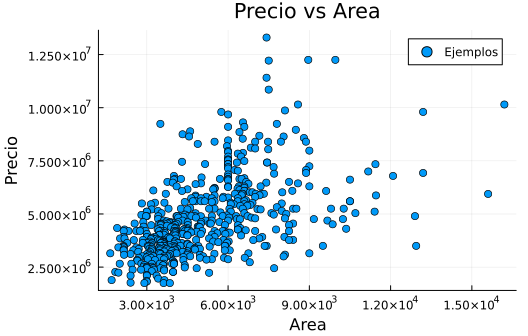
\includegraphics[keepaspectratio]{index_files/mediabag/03-regresion_files/figure-pdf/cell-3-output-1.pdf}}

  \end{tcolorbox}
\item
  Definir un modelo lineal que explique el precio en función del área de
  las viviendas.

  \begin{tcolorbox}[enhanced jigsaw, toptitle=1mm, colframe=quarto-callout-note-color-frame, titlerule=0mm, left=2mm, arc=.35mm, colbacktitle=quarto-callout-note-color!10!white, opacityback=0, bottomtitle=1mm, toprule=.15mm, coltitle=black, breakable, colback=white, rightrule=.15mm, opacitybacktitle=0.6, leftrule=.75mm, bottomrule=.15mm, title=\textcolor{quarto-callout-note-color}{\faInfo}\hspace{0.5em}{Ayuda}]

  Un modelo lineal tiene encuación \(y = \theta_1 + \theta_2 x\).

  \end{tcolorbox}

  \begin{tcolorbox}[enhanced jigsaw, toptitle=1mm, colframe=quarto-callout-tip-color-frame, titlerule=0mm, left=2mm, arc=.35mm, colbacktitle=quarto-callout-tip-color!10!white, opacityback=0, bottomtitle=1mm, toprule=.15mm, coltitle=black, breakable, colback=white, rightrule=.15mm, opacitybacktitle=0.6, leftrule=.75mm, bottomrule=.15mm, title=\textcolor{quarto-callout-tip-color}{\faLightbulb}\hspace{0.5em}{Solución}]

\begin{Shaded}
\begin{Highlighting}[]
\FunctionTok{precio}\NormalTok{(area, θ) }\OperatorTok{=}\NormalTok{ θ[}\FloatTok{1}\NormalTok{] }\OperatorTok{.+}\NormalTok{ θ[}\FloatTok{2}\NormalTok{] }\OperatorTok{*}\NormalTok{ area}
\end{Highlighting}
\end{Shaded}

\begin{verbatim}
precio (generic function with 1 method)
\end{verbatim}

  Observa que la función precio está vectorizada, lo que significa que
  puede recibir un vector de áreas y devolver un vector de precios.

  \end{tcolorbox}
\item
  Inicializar los parámetros del modelo lineal con valores nulos y
  dibujar el modelo sobre el diagrama de dispersión.

  \begin{tcolorbox}[enhanced jigsaw, toptitle=1mm, colframe=quarto-callout-tip-color-frame, titlerule=0mm, left=2mm, arc=.35mm, colbacktitle=quarto-callout-tip-color!10!white, opacityback=0, bottomtitle=1mm, toprule=.15mm, coltitle=black, breakable, colback=white, rightrule=.15mm, opacitybacktitle=0.6, leftrule=.75mm, bottomrule=.15mm, title=\textcolor{quarto-callout-tip-color}{\faLightbulb}\hspace{0.5em}{Solución}]

\begin{Shaded}
\begin{Highlighting}[]
\NormalTok{θ }\OperatorTok{=}\NormalTok{ [}\FloatTok{0.0}\NormalTok{, }\FloatTok{0.0}\NormalTok{]}
\FunctionTok{plot!}\NormalTok{(df.area, }\FunctionTok{precio}\NormalTok{(df.area, θ), label }\OperatorTok{=} \StringTok{"Modelo 0"}\NormalTok{)}
\end{Highlighting}
\end{Shaded}

  \pandocbounded{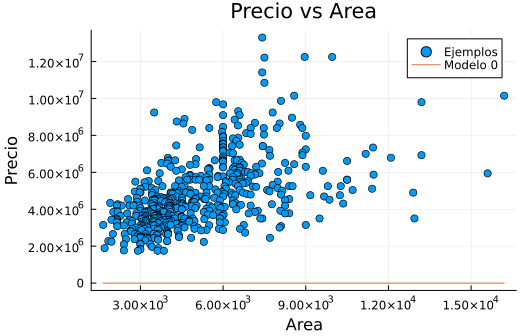
\includegraphics[keepaspectratio]{index_files/mediabag/03-regresion_files/figure-pdf/cell-5-output-1.pdf}}

  \end{tcolorbox}
\item
  Definir una función de costo para el modelo lineal y evaluar el coste
  para el modelo lineal construido con los parámetros iniciales. A la
  vista del coste obtenido, ¿cómo de bueno es el modelo?

  \begin{tcolorbox}[enhanced jigsaw, toptitle=1mm, colframe=quarto-callout-note-color-frame, titlerule=0mm, left=2mm, arc=.35mm, colbacktitle=quarto-callout-note-color!10!white, opacityback=0, bottomtitle=1mm, toprule=.15mm, coltitle=black, breakable, colback=white, rightrule=.15mm, opacitybacktitle=0.6, leftrule=.75mm, bottomrule=.15mm, title=\textcolor{quarto-callout-note-color}{\faInfo}\hspace{0.5em}{Ayuda}]

  La función de coste para un modelo lineal es el error cuadrático
  medio.

  \[ J(\theta) = \frac{1}{2m} \sum_{i=1}^{m} (h_\theta(x^{(i)}) - y^{(i)})^2 \]

  donde \(h_\theta\) es el modelo, \(h_\theta(x^{(i)})\) es la
  predicción del modelo para el ejemplo \(i\)-ésimo, \(y^{(i)}\) es el
  valor real observado para el ejemplo \(i\)-ésimo, y \(m\) es el número
  de ejemplos.

  \end{tcolorbox}

  \begin{tcolorbox}[enhanced jigsaw, toptitle=1mm, colframe=quarto-callout-tip-color-frame, titlerule=0mm, left=2mm, arc=.35mm, colbacktitle=quarto-callout-tip-color!10!white, opacityback=0, bottomtitle=1mm, toprule=.15mm, coltitle=black, breakable, colback=white, rightrule=.15mm, opacitybacktitle=0.6, leftrule=.75mm, bottomrule=.15mm, title=\textcolor{quarto-callout-tip-color}{\faLightbulb}\hspace{0.5em}{Solución}]

\begin{Shaded}
\begin{Highlighting}[]
\KeywordTok{function} \FunctionTok{coste}\NormalTok{(θ, X, Y)}
\NormalTok{    m }\OperatorTok{=} \FunctionTok{length}\NormalTok{(Y)}
    \ControlFlowTok{return} \FunctionTok{sum}\NormalTok{((}\FunctionTok{precio}\NormalTok{(X, θ) }\OperatorTok{.{-}}\NormalTok{ Y)}\OperatorTok{.\^{}}\FloatTok{2}\NormalTok{) }\OperatorTok{/}\NormalTok{ (}\FloatTok{2} \OperatorTok{*}\NormalTok{ m)}
\KeywordTok{end}

\FunctionTok{coste}\NormalTok{(θ, df.area, df.precio)}
\end{Highlighting}
\end{Shaded}

\begin{verbatim}
1.3106916364659266e13
\end{verbatim}

  La función de coste nos da una medida de lo lejos que están las
  predicciones del modelo de los valores reales observados. En este
  caso, el coste es muy alto, lo que indica que el modelo no es bueno.

  \end{tcolorbox}
\item
  ¿En qué dirección debemos modificar los parámetros del modelo para
  mejorar el modelo?

  \begin{tcolorbox}[enhanced jigsaw, toptitle=1mm, colframe=quarto-callout-tip-color-frame, titlerule=0mm, left=2mm, arc=.35mm, colbacktitle=quarto-callout-tip-color!10!white, opacityback=0, bottomtitle=1mm, toprule=.15mm, coltitle=black, breakable, colback=white, rightrule=.15mm, opacitybacktitle=0.6, leftrule=.75mm, bottomrule=.15mm, title=\textcolor{quarto-callout-tip-color}{\faLightbulb}\hspace{0.5em}{Solución}]

  Para minimizar la función de coste, debemos modificar los parámetros
  del modelo en la dirección opuesta al gradiente de la función de
  coste, ya que el gradiente de una función indica la dirección de mayor
  crecimiento de la función.

  \end{tcolorbox}
\item
  Crear una función para modificar los pesos del modelo lineal mediante
  el algoritmo del gradiente descendente, y aplicarla a los parámetros
  actuales tomando una tasa de aprendizaje de \(10^{-8}\). ¿Cómo han
  cambiado los parámetros del modelo? Dibujar el modelo actualizado
  sobre el diagrama de dispersión. ¿Cómo ha cambiado el coste?

  \begin{tcolorbox}[enhanced jigsaw, toptitle=1mm, colframe=quarto-callout-note-color-frame, titlerule=0mm, left=2mm, arc=.35mm, colbacktitle=quarto-callout-note-color!10!white, opacityback=0, bottomtitle=1mm, toprule=.15mm, coltitle=black, breakable, colback=white, rightrule=.15mm, opacitybacktitle=0.6, leftrule=.75mm, bottomrule=.15mm, title=\textcolor{quarto-callout-note-color}{\faInfo}\hspace{0.5em}{Ayuda}]

  El algoritmo del gradiente descendente actualiza los parámetros del
  modelo de acuerdo a la siguiente regla:

  \[
  \theta_j = \theta_j - \alpha \frac{\partial J(\theta)}{\partial \theta_j}
  \]

  donde \(\alpha\) es la tasa de aprendizaje y
  \(\frac{\partial J(\theta)}{\partial \theta_j}\) es la derivada
  parcial de la función de coste con respecto al parámetro \(\theta_j\).

  \end{tcolorbox}

  \begin{tcolorbox}[enhanced jigsaw, toptitle=1mm, colframe=quarto-callout-tip-color-frame, titlerule=0mm, left=2mm, arc=.35mm, colbacktitle=quarto-callout-tip-color!10!white, opacityback=0, bottomtitle=1mm, toprule=.15mm, coltitle=black, breakable, colback=white, rightrule=.15mm, opacitybacktitle=0.6, leftrule=.75mm, bottomrule=.15mm, title=\textcolor{quarto-callout-tip-color}{\faLightbulb}\hspace{0.5em}{Solución}]

\begin{Shaded}
\begin{Highlighting}[]
\KeywordTok{function} \FunctionTok{gradiente\_descendente!}\NormalTok{(θ, X, Y, α)}
    \CommentTok{\# Calculamos el número de ejemplos}
\NormalTok{    m }\OperatorTok{=} \FunctionTok{length}\NormalTok{(Y)}
    \CommentTok{\# Actualizamos el término independiente del modelo lineal.}
\NormalTok{    θ[}\FloatTok{1}\NormalTok{] }\OperatorTok{{-}=}\NormalTok{ α }\OperatorTok{*} \FunctionTok{sum}\NormalTok{(}\FunctionTok{precio}\NormalTok{(X, θ) }\OperatorTok{{-}}\NormalTok{ Y) }\OperatorTok{/}\NormalTok{ m}
    \CommentTok{\# Actualizamos la pendiente del modelo lineal.}
\NormalTok{    θ[}\FloatTok{2}\NormalTok{] }\OperatorTok{{-}=}\NormalTok{ α }\OperatorTok{*} \FunctionTok{sum}\NormalTok{((}\FunctionTok{precio}\NormalTok{(X, θ) }\OperatorTok{{-}}\NormalTok{ Y) }\OperatorTok{.*}\NormalTok{ X) }\OperatorTok{/}\NormalTok{ m}
    \ControlFlowTok{return}\NormalTok{ θ}
\KeywordTok{end}
\end{Highlighting}
\end{Shaded}

\begin{verbatim}
gradiente_descendente! (generic function with 1 method)
\end{verbatim}

  Aplicamos la función a los parámetros del modelo actual y mostramos
  los nuevos parámetros.

\begin{Shaded}
\begin{Highlighting}[]
\FunctionTok{gradiente\_descendente!}\NormalTok{(θ, df.area, df.precio, }\FloatTok{1e{-}8}\NormalTok{)}
\NormalTok{θ}
\end{Highlighting}
\end{Shaded}

\begin{verbatim}
2-element Vector{Float64}:
   0.04766729247706422
 267.22919804579385
\end{verbatim}

  Dibujamos el nuevo modelo.

\begin{Shaded}
\begin{Highlighting}[]
\FunctionTok{plot!}\NormalTok{(df.area, }\FunctionTok{precio}\NormalTok{(df.area, θ), label }\OperatorTok{=} \StringTok{"Modelo 1"}\NormalTok{)}
\end{Highlighting}
\end{Shaded}

  \pandocbounded{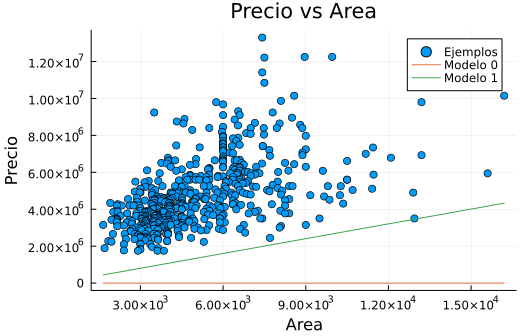
\includegraphics[keepaspectratio]{index_files/mediabag/03-regresion_files/figure-pdf/cell-9-output-1.pdf}}

  Se observa que ahora la recta está más cerca de la nube de puntos, por
  lo que el modelo ha mejorado. Calculamos el coste del nuevo modelo.

\begin{Shaded}
\begin{Highlighting}[]
\FunctionTok{coste}\NormalTok{(θ, df.area, df.precio)}
\end{Highlighting}
\end{Shaded}

\begin{verbatim}
7.080823787113201e12
\end{verbatim}

  \end{tcolorbox}
\item
  Repetir el proceso de actualización de los parámetros del modelo
  mediante el algoritmo del gradiente descendente durante 9 iteraciones
  más y dibujar los modelos actualizados.

  \begin{tcolorbox}[enhanced jigsaw, toptitle=1mm, colframe=quarto-callout-tip-color-frame, titlerule=0mm, left=2mm, arc=.35mm, colbacktitle=quarto-callout-tip-color!10!white, opacityback=0, bottomtitle=1mm, toprule=.15mm, coltitle=black, breakable, colback=white, rightrule=.15mm, opacitybacktitle=0.6, leftrule=.75mm, bottomrule=.15mm, title=\textcolor{quarto-callout-tip-color}{\faLightbulb}\hspace{0.5em}{Solución}]

\begin{Shaded}
\begin{Highlighting}[]
\ControlFlowTok{for}\NormalTok{ i }\OperatorTok{=} \FloatTok{2}\OperatorTok{:}\FloatTok{10}
    \FunctionTok{gradiente\_descendente!}\NormalTok{(θ, df.area, df.precio, }\FloatTok{1e{-}8}\NormalTok{)}
    \FunctionTok{plot!}\NormalTok{(df.area, }\FunctionTok{precio}\NormalTok{(df.area, θ), label }\OperatorTok{=} \StringTok{"Modelo }\SpecialCharTok{$}\NormalTok{i}\StringTok{"}\NormalTok{, legend }\OperatorTok{=} \ConstantTok{true}\NormalTok{)}
\ControlFlowTok{end}
\NormalTok{plt}
\end{Highlighting}
\end{Shaded}

  \pandocbounded{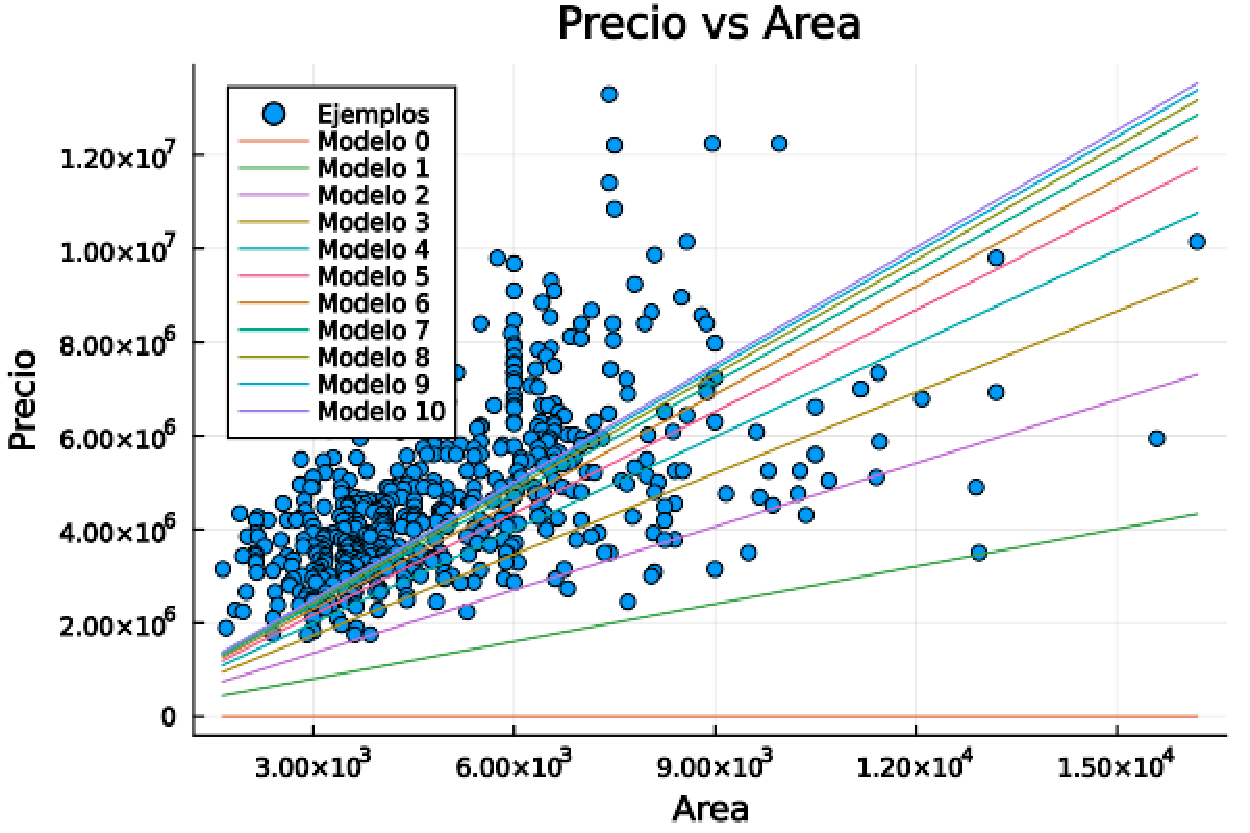
\includegraphics[keepaspectratio]{img/regresion/modelos_regresion.pdf}}

  \end{tcolorbox}
\item
  Dibujar un gráfico con la evolución del coste del modelo a lo largo de
  las iteraciones. ¿Cómo se comporta el coste a lo largo de las
  iteraciones?

  \begin{tcolorbox}[enhanced jigsaw, toptitle=1mm, colframe=quarto-callout-tip-color-frame, titlerule=0mm, left=2mm, arc=.35mm, colbacktitle=quarto-callout-tip-color!10!white, opacityback=0, bottomtitle=1mm, toprule=.15mm, coltitle=black, breakable, colback=white, rightrule=.15mm, opacitybacktitle=0.6, leftrule=.75mm, bottomrule=.15mm, title=\textcolor{quarto-callout-tip-color}{\faLightbulb}\hspace{0.5em}{Solución}]

\begin{Shaded}
\begin{Highlighting}[]
\NormalTok{costes }\OperatorTok{=} \DataTypeTok{Float64}\NormalTok{[]}
\ControlFlowTok{for}\NormalTok{ i }\OperatorTok{=} \FloatTok{1}\OperatorTok{:}\FloatTok{10}
    \FunctionTok{gradiente\_descendente!}\NormalTok{(θ, df.area, df.precio, }\FloatTok{1e{-}8}\NormalTok{)}
    \FunctionTok{push!}\NormalTok{(costes, }\FunctionTok{coste}\NormalTok{(θ, df.area, df.precio))}
\ControlFlowTok{end}
\NormalTok{costes}
\end{Highlighting}
\end{Shaded}

\begin{verbatim}
10-element Vector{Float64}:
 4.230808760870044e12
 2.882906194020343e12
 2.2454213686913755e12
 1.9439256128790886e12
 1.8013344680594421e12
 1.7338965877160208e12
 1.7020021263374993e12
 1.6869177748236997e12
 1.6797836937723748e12
 1.6764096595632322e12
\end{verbatim}

  El coste del modelo disminuye en cada iteración, lo que indica que el
  modelo está mejorando. Esto se debe a que el algoritmo del gradiente
  descendente modifica los parámetros del modelo en la dirección que
  minimiza la función de coste.

  \end{tcolorbox}
\item
  ¿Hasta qué iteración habrá que llegar para conseguir un reducción del
  coste menor de un \(0.0001\%\)?

  \begin{tcolorbox}[enhanced jigsaw, toptitle=1mm, colframe=quarto-callout-tip-color-frame, titlerule=0mm, left=2mm, arc=.35mm, colbacktitle=quarto-callout-tip-color!10!white, opacityback=0, bottomtitle=1mm, toprule=.15mm, coltitle=black, breakable, colback=white, rightrule=.15mm, opacitybacktitle=0.6, leftrule=.75mm, bottomrule=.15mm, title=\textcolor{quarto-callout-tip-color}{\faLightbulb}\hspace{0.5em}{Solución}]

\begin{Shaded}
\begin{Highlighting}[]
\NormalTok{θ }\OperatorTok{=}\NormalTok{ [}\FloatTok{0.0}\NormalTok{, }\FloatTok{0.0}\NormalTok{]}
\NormalTok{costes }\OperatorTok{=}\NormalTok{ [}\FloatTok{0}\NormalTok{, }\FunctionTok{coste}\NormalTok{(θ, df.area, df.precio)]}
\NormalTok{i }\OperatorTok{=} \FloatTok{1}
\ControlFlowTok{while} \FunctionTok{abs}\NormalTok{(costes[}\KeywordTok{end}\NormalTok{] }\OperatorTok{{-}}\NormalTok{ costes[}\KeywordTok{end}\OperatorTok{{-}}\FloatTok{1}\NormalTok{]) }\OperatorTok{/}\NormalTok{ costes[}\KeywordTok{end}\OperatorTok{{-}}\FloatTok{1}\NormalTok{] }\OperatorTok{\textgreater{}} \FloatTok{0.000001}
\NormalTok{    i }\OperatorTok{+=} \FloatTok{1}
    \FunctionTok{gradiente\_descendente!}\NormalTok{(θ, df.area, df.precio, }\FloatTok{1e{-}8}\NormalTok{)}
    \FunctionTok{push!}\NormalTok{(costes, }\FunctionTok{coste}\NormalTok{(θ, df.area, df.precio))}
\ControlFlowTok{end}
\NormalTok{i}
\end{Highlighting}
\end{Shaded}

\begin{verbatim}
23
\end{verbatim}

  En este caso, el algoritmo del gradiente descendente converge en 1000
  iteraciones.

  \end{tcolorbox}
\item
  ¿Qué sucede si se utiliza una tasa de aprendizaje \(\alpha = 0.0001\)?
  ¿Cómo afecta al coste y a la convergencia del modelo?

  \begin{tcolorbox}[enhanced jigsaw, toptitle=1mm, colframe=quarto-callout-tip-color-frame, titlerule=0mm, left=2mm, arc=.35mm, colbacktitle=quarto-callout-tip-color!10!white, opacityback=0, bottomtitle=1mm, toprule=.15mm, coltitle=black, breakable, colback=white, rightrule=.15mm, opacitybacktitle=0.6, leftrule=.75mm, bottomrule=.15mm, title=\textcolor{quarto-callout-tip-color}{\faLightbulb}\hspace{0.5em}{Solución}]

\begin{Shaded}
\begin{Highlighting}[]
\NormalTok{θ }\OperatorTok{=}\NormalTok{ [}\FloatTok{0.0}\NormalTok{, }\FloatTok{0.0}\NormalTok{]}
\NormalTok{costes }\OperatorTok{=}\NormalTok{ [}\FunctionTok{coste}\NormalTok{(θ, df.area, df.precio)]}
\ControlFlowTok{for}\NormalTok{ i }\OperatorTok{=} \FloatTok{1}\OperatorTok{:}\FloatTok{10}
    \FunctionTok{gradiente\_descendente!}\NormalTok{(θ, df.area, df.precio, }\FloatTok{0.0001}\NormalTok{)}
    \FunctionTok{push!}\NormalTok{(costes, }\FunctionTok{coste}\NormalTok{(θ, df.area, df.precio))}
\ControlFlowTok{end}
\NormalTok{costes}
\end{Highlighting}
\end{Shaded}

\begin{verbatim}
11-element Vector{Float64}:
 1.3106916364659266e13
 1.114133369099188e20
 1.0856750832581238e27
 1.05794371802143e34
 1.0309206941949286e41
 1.004587918634273e48
 9.789277603492545e54
 9.539230386975057e61
 9.29557011881276e68
 9.058133657380397e75
 8.826762028174244e82
\end{verbatim}

  Si la tasa de aprendizaje es demasiado grande, el algoritmo del
  gradiente descendente puede no converger y el coste puede oscilar en
  lugar de disminuir. En este caso, el coste aumenta en cada iteración,
  lo que indica que la tasa de aprendizaje es demasiado grande.

  \end{tcolorbox}
\end{enumerate}

\end{exercise}

\bookmarksetup{startatroot}

\chapter{Árboles de decisión}\label{uxe1rboles-de-decisiuxf3n}

Los árboles de decisión son modelos de aprendizaje simples e intuitivos
que pueden utilizarse para tanto para predecir variables cuantitativas
(regresión) como categóricas (clasificación). Esta práctica contiene
ejercicios que muestran como construir modelos de aprendizaje basados en
árboles de decisión con Julia.

\section{Ejercicios Resueltos}\label{ejercicios-resueltos-2}

Para la realización de esta práctica se requieren los siguientes
paquetes:

\begin{Shaded}
\begin{Highlighting}[]
\ImportTok{using} \BuiltInTok{CSV}  \CommentTok{\# Para la lectura de archivos CSV.}
\ImportTok{using} \BuiltInTok{DataFrames}  \CommentTok{\# Para el manejo de datos tabulares.}
\ImportTok{using} \BuiltInTok{Tidier} \CommentTok{\# Para el preprocesamiento de datos.}
\ImportTok{using} \BuiltInTok{PrettyTables}  \CommentTok{\# Para mostrar tablas formateadas.}
\ImportTok{using} \BuiltInTok{Plots}  \CommentTok{\# Para el dibujo de gráficas.}
\ImportTok{using} \BuiltInTok{GLMakie}  \CommentTok{\# Para obtener gráficos interactivos.}
\ImportTok{using} \BuiltInTok{AlgebraOfGraphics} \CommentTok{\# Para generar gráficos mediante la gramática de gráficos.}
\ImportTok{using} \BuiltInTok{DecisionTree} \CommentTok{\# Para construir árboles de decisión.}
\ImportTok{using} \BuiltInTok{GraphMakie} \CommentTok{\# Para la visualización de árboles de decisión.}
\end{Highlighting}
\end{Shaded}

\begin{exercise}[]\protect\hypertarget{exr-arboles-decision-1}{}\label{exr-arboles-decision-1}

El conjunto de datos \href{./datos/tenis.csv}{\texttt{tenis.csv}}
contiene información sobre las condiciones meteorológicas de varios días
y si se pudo jugar al tenis o no.

\begin{enumerate}
\def\labelenumi{\alph{enumi}.}
\item
  Cargar los datos del archivo \texttt{tenis.csv} en un data frame.

  \begin{tcolorbox}[enhanced jigsaw, toptitle=1mm, colframe=quarto-callout-tip-color-frame, titlerule=0mm, left=2mm, arc=.35mm, colbacktitle=quarto-callout-tip-color!10!white, opacityback=0, bottomtitle=1mm, toprule=.15mm, coltitle=black, breakable, colback=white, rightrule=.15mm, opacitybacktitle=0.6, leftrule=.75mm, bottomrule=.15mm, title=\textcolor{quarto-callout-tip-color}{\faLightbulb}\hspace{0.5em}{Solución}]

\begin{Shaded}
\begin{Highlighting}[]
\ImportTok{using} \BuiltInTok{CSV}\NormalTok{, }\BuiltInTok{DataFrames}
\NormalTok{df }\OperatorTok{=}\NormalTok{ CSV.}\FunctionTok{read}\NormalTok{(}\StringTok{"datos/tenis.csv"}\NormalTok{, DataFrame)}
\end{Highlighting}
\end{Shaded}

  \begin{tabular}{r|ccccc}
      & Cielo & Temperatura & Humedad & Viento & Tenis\\
      \hline
      & String15 & String15 & String7 & String7 & String3\\
      \hline
      1 & Soleado & Caluroso & Alta & Suave & No \\
      2 & Soleado & Caluroso & Alta & Fuerte & No \\
      3 & Nublado & Caluroso & Alta & Suave & Sí \\
      4 & Lluvioso & Moderado & Alta & Suave & Sí \\
      5 & Lluvioso & Frío & Normal & Suave & Sí \\
      6 & Lluvioso & Frío & Normal & Fuerte & No \\
      7 & Nublado & Frío & Normal & Fuerte & Sí \\
      8 & Soleado & Moderado & Alta & Suave & No \\
      9 & Soleado & Frío & Normal & Suave & Sí \\
      10 & Lluvioso & Moderado & Normal & Suave & Sí \\
      11 & Soleado & Moderado & Normal & Fuerte & Sí \\
      12 & Nublado & Moderado & Alta & Fuerte & Sí \\
      13 & Nublado & Caluroso & Normal & Suave & Sí \\
      14 & Lluvioso & Moderado & Alta & Fuerte & No \\
  \end{tabular}

  \end{tcolorbox}
\item
  Crear un diagrama de barras que muestre la distribución de frecuencias
  de cada variable meteorológica según si se pudo jugar al tenis o no.
  ¿Qué variable meteorológica parece tener más influencia en la decisión
  de jugar al tenis?

  \begin{tcolorbox}[enhanced jigsaw, toptitle=1mm, colframe=quarto-callout-tip-color-frame, titlerule=0mm, left=2mm, arc=.35mm, colbacktitle=quarto-callout-tip-color!10!white, opacityback=0, bottomtitle=1mm, toprule=.15mm, coltitle=black, breakable, colback=white, rightrule=.15mm, opacitybacktitle=0.6, leftrule=.75mm, bottomrule=.15mm, title=\textcolor{quarto-callout-tip-color}{\faLightbulb}\hspace{0.5em}{Solución}]

\begin{Shaded}
\begin{Highlighting}[]
\ImportTok{using} \BuiltInTok{GLMakie}\NormalTok{, }\BuiltInTok{AlgebraOfGraphics}

\KeywordTok{function} \FunctionTok{frecuencias}\NormalTok{(df}\OperatorTok{::}\DataTypeTok{DataFrame}\NormalTok{, var}\OperatorTok{::}\DataTypeTok{Symbol}\NormalTok{)}
    \CommentTok{\# Calculamos el número de días de cada clase que se juega al tenis.}
\NormalTok{    frec }\OperatorTok{=} \FunctionTok{combine}\NormalTok{(}\FunctionTok{groupby}\NormalTok{(df, [var, }\OperatorTok{:}\NormalTok{Tenis]), nrow }\OperatorTok{=\textgreater{}} \OperatorTok{:}\NormalTok{Días)}
    \CommentTok{\# Dibujamos el diagrama de barras.}
\NormalTok{    plt }\OperatorTok{=} \FunctionTok{data}\NormalTok{(frec) }\OperatorTok{*} 
    \FunctionTok{mapping}\NormalTok{(var, }\OperatorTok{:}\NormalTok{Días, stack }\OperatorTok{=} \OperatorTok{:}\NormalTok{Tenis, color }\OperatorTok{=} \OperatorTok{:}\NormalTok{Tenis, ) }\OperatorTok{*} 
    \FunctionTok{visual}\NormalTok{(BarPlot) }
    \CommentTok{\# Devolvemos el gráfico.}
    \ControlFlowTok{return}\NormalTok{ plt}
\KeywordTok{end}

\NormalTok{fig }\OperatorTok{=} \FunctionTok{Figure}\NormalTok{()}
\FunctionTok{draw!}\NormalTok{(fig[}\FloatTok{1}\NormalTok{, }\FloatTok{1}\NormalTok{], }\FunctionTok{frecuencias}\NormalTok{(df, }\OperatorTok{:}\NormalTok{Cielo))}
\FunctionTok{draw!}\NormalTok{(fig[}\FloatTok{1}\NormalTok{, }\FloatTok{2}\NormalTok{], }\FunctionTok{frecuencias}\NormalTok{(df, }\OperatorTok{:}\NormalTok{Temperatura))}
\FunctionTok{draw!}\NormalTok{(fig[}\FloatTok{1}\NormalTok{, }\FloatTok{3}\NormalTok{], }\FunctionTok{frecuencias}\NormalTok{(df, }\OperatorTok{:}\NormalTok{Humedad))}
\FunctionTok{draw!}\NormalTok{(fig[}\FloatTok{1}\NormalTok{, }\FloatTok{4}\NormalTok{], }\FunctionTok{frecuencias}\NormalTok{(df, }\OperatorTok{:}\NormalTok{Viento))}
\NormalTok{fig}
\end{Highlighting}
\end{Shaded}

  \pandocbounded{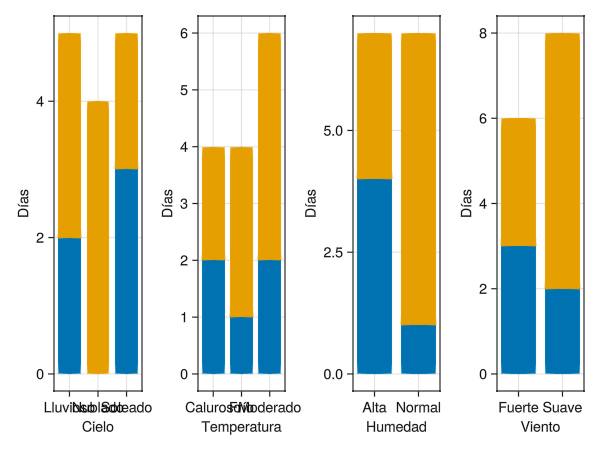
\includegraphics[keepaspectratio]{07-arboles-decision_files/figure-pdf/cell-3-output-1.png}}

  A la vista de las frecuencias de cada variable, las variable
  \texttt{Cielo} y \texttt{Humedad} parecen ser las que más influye en
  la decisión de jugar al tenis.

  \end{tcolorbox}
\item
  Calcular la impureza del conjunto de datos utilizando el índice de
  Gini. ¿Qué variable meteorológica parece tener más influencia en la
  decisión de jugar al tenis?

  \begin{tcolorbox}[enhanced jigsaw, toptitle=1mm, colframe=quarto-callout-note-color-frame, titlerule=0mm, left=2mm, arc=.35mm, colbacktitle=quarto-callout-note-color!10!white, opacityback=0, bottomtitle=1mm, toprule=.15mm, coltitle=black, breakable, colback=white, rightrule=.15mm, opacitybacktitle=0.6, leftrule=.75mm, bottomrule=.15mm, title=\textcolor{quarto-callout-note-color}{\faInfo}\hspace{0.5em}{Ayuda}]

  El
  \href{https://en.wikipedia.org/wiki/Decision_tree_learning\#Gini_impurity}{índice
  de Gini} se calcula mediante la fórmula

  \[ GI = 1 - \sum_{i=1}^{n} p_i^2 \]

  donde \(p_i\) es la proporción de cada clase en el conjunto de datos y
  \(n\) es el número de clases.

  El índice de Gini toma valores entre \(0\) y \(1-\frac{1}{n}\)
  (\(0.5\) en el caso de clasificación binaria), donde \(0\) indica que
  todas las instancias pertenecen a una sola clase (mínima impureza) y
  \(1-\frac{1}{n}\) indica que las instancias están distribuidas
  uniformemente entre todas las clases (máxima impureza).

  \end{tcolorbox}

  \begin{tcolorbox}[enhanced jigsaw, toptitle=1mm, colframe=quarto-callout-tip-color-frame, titlerule=0mm, left=2mm, arc=.35mm, colbacktitle=quarto-callout-tip-color!10!white, opacityback=0, bottomtitle=1mm, toprule=.15mm, coltitle=black, breakable, colback=white, rightrule=.15mm, opacitybacktitle=0.6, leftrule=.75mm, bottomrule=.15mm, title=\textcolor{quarto-callout-tip-color}{\faLightbulb}\hspace{0.5em}{Solución}]

\begin{Shaded}
\begin{Highlighting}[]
\KeywordTok{function} \FunctionTok{gini}\NormalTok{(df}\OperatorTok{::}\DataTypeTok{DataFrame}\NormalTok{, var}\OperatorTok{::}\DataTypeTok{Symbol}\NormalTok{)}
    \CommentTok{\# Calculamos el número de ejemplos.}
\NormalTok{    n }\OperatorTok{=} \FunctionTok{nrow}\NormalTok{(df)}
    \CommentTok{\# Calculamos las frecuencias absolutas de cada clase.}
\NormalTok{    frec }\OperatorTok{=} \FunctionTok{combine}\NormalTok{(}\FunctionTok{groupby}\NormalTok{(df, var), nrow }\OperatorTok{=\textgreater{}} \OperatorTok{:}\NormalTok{ni)}
    \CommentTok{\# Calculamos la proporción de cada clase.}
\NormalTok{    frec.p }\OperatorTok{=}\NormalTok{ frec.ni }\OperatorTok{./}\NormalTok{ n}
    \CommentTok{\# Calculamos el índice de Gini.}
\NormalTok{    gini }\OperatorTok{=} \FloatTok{1} \OperatorTok{{-}} \FunctionTok{sum}\NormalTok{(frec.p }\OperatorTok{.\^{}} \FloatTok{2}\NormalTok{)}
    \ControlFlowTok{return}\NormalTok{ gini}
\KeywordTok{end}

\NormalTok{g0 }\OperatorTok{=} \FunctionTok{gini}\NormalTok{(df, }\OperatorTok{:}\NormalTok{Tenis)}
\end{Highlighting}
\end{Shaded}

\begin{verbatim}
0.4591836734693877
\end{verbatim}

  \end{tcolorbox}
\item
  ¿Qué reducción del índice Gini se obtiene si dividimos el conjunto de
  ejemplos según la variable \texttt{Humedad}? ¿Y si dividimos el
  conjunto con respecto a la variable \texttt{Viento}?

  \begin{tcolorbox}[enhanced jigsaw, toptitle=1mm, colframe=quarto-callout-note-color-frame, titlerule=0mm, left=2mm, arc=.35mm, colbacktitle=quarto-callout-note-color!10!white, opacityback=0, bottomtitle=1mm, toprule=.15mm, coltitle=black, breakable, colback=white, rightrule=.15mm, opacitybacktitle=0.6, leftrule=.75mm, bottomrule=.15mm, title=\textcolor{quarto-callout-note-color}{\faInfo}\hspace{0.5em}{Ayuda}]

  La reducción del índice de Gini se calcula como la diferencia entre el
  índice de Gini del conjunto original y el índice de Gini del conjunto
  dividido.

  \[ \Delta GI = GI_{original} - GI_{dividido} \]

  donde el índice de Gini del conjunto dividido es la media ponderada de
  los índices de Gini de los subconjuntos resultantes de la división.

  \end{tcolorbox}

  \begin{tcolorbox}[enhanced jigsaw, toptitle=1mm, colframe=quarto-callout-tip-color-frame, titlerule=0mm, left=2mm, arc=.35mm, colbacktitle=quarto-callout-tip-color!10!white, opacityback=0, bottomtitle=1mm, toprule=.15mm, coltitle=black, breakable, colback=white, rightrule=.15mm, opacitybacktitle=0.6, leftrule=.75mm, bottomrule=.15mm, title=\textcolor{quarto-callout-tip-color}{\faLightbulb}\hspace{0.5em}{Solución}]

  Calculamos primero la reducción del índice de Gini al dividir el
  conjunto de ejemplos según la variable \texttt{Humedad}.

\begin{Shaded}
\begin{Highlighting}[]
\ImportTok{using} \BuiltInTok{Tidier}
\CommentTok{\# Dividimos el conjunto de ejemplos según la variable Humedad.}
\NormalTok{df\_humedad\_alta }\OperatorTok{=} \PreprocessorTok{@filter}\NormalTok{(df, Humedad }\OperatorTok{==} \StringTok{"Alta"}\NormalTok{)}
\NormalTok{df\_humedad\_normal }\OperatorTok{=} \PreprocessorTok{@filter}\NormalTok{(df, Humedad }\OperatorTok{==} \StringTok{"Normal"}\NormalTok{)}
\CommentTok{\# Calculamos los tamaños de los subconjuntos de ejemplos.}
\NormalTok{n }\OperatorTok{=} \FunctionTok{nrow}\NormalTok{(df\_humedad\_alta), }\FunctionTok{nrow}\NormalTok{(df\_humedad\_normal)}
\CommentTok{\# Calculamos el índice de Gini de cada subconjunto.}
\NormalTok{gis }\OperatorTok{=} \FunctionTok{gini}\NormalTok{(df\_humedad\_alta, }\OperatorTok{:}\NormalTok{Tenis), }\FunctionTok{gini}\NormalTok{(df\_humedad\_normal, }\OperatorTok{:}\NormalTok{Tenis)}
\CommentTok{\# Calculamos media ponderada de los índices de Gini de los subconjuntos }
\NormalTok{g\_humedad }\OperatorTok{=} \FunctionTok{sum}\NormalTok{(gis }\OperatorTok{.*}\NormalTok{ n) }\OperatorTok{/} \FunctionTok{sum}\NormalTok{(n)}
\CommentTok{\# Calculamos la reducción del índice de Gini.}
\NormalTok{g0 }\OperatorTok{{-}}\NormalTok{ g\_humedad}
\end{Highlighting}
\end{Shaded}

\begin{verbatim}
0.09183673469387743
\end{verbatim}

  Calculamos ahora la reducción del índice de Gini al dividir el
  conjunto de ejemplos según la variable \texttt{Viento}.

\begin{Shaded}
\begin{Highlighting}[]
\CommentTok{\# Dividimos el conjunto de ejemplos según la variable \textasciigrave{}Viento\textasciigrave{}}
\NormalTok{df\_viento\_fuerte }\OperatorTok{=} \PreprocessorTok{@filter}\NormalTok{(df, Viento }\OperatorTok{==} \StringTok{"Fuerte"}\NormalTok{)}
\NormalTok{df\_viento\_suave }\OperatorTok{=} \PreprocessorTok{@filter}\NormalTok{(df, Viento }\OperatorTok{==} \StringTok{"Suave"}\NormalTok{)}
\CommentTok{\# Calculamos los tamaños de los subconjuntos de ejemplos}
\NormalTok{n }\OperatorTok{=} \FunctionTok{nrow}\NormalTok{(df\_viento\_fuerte), }\FunctionTok{nrow}\NormalTok{(df\_viento\_suave)}
\CommentTok{\# Calculamos el índice de Gini de cada subconjunto}
\NormalTok{gis }\OperatorTok{=} \FunctionTok{gini}\NormalTok{(df\_viento\_fuerte, }\OperatorTok{:}\NormalTok{Tenis), }\FunctionTok{gini}\NormalTok{(df\_viento\_suave, }\OperatorTok{:}\NormalTok{Tenis)}
\CommentTok{\# Calculamos media ponderada de los índices de Gini de los subconjuntos}
\NormalTok{g\_viento }\OperatorTok{=} \FunctionTok{sum}\NormalTok{(gis }\OperatorTok{.*}\NormalTok{ n) }\OperatorTok{/} \FunctionTok{sum}\NormalTok{(n)}
\CommentTok{\# Calculamos la reducción del índice de Gini}
\NormalTok{g0 }\OperatorTok{{-}}\NormalTok{ g\_viento}
\end{Highlighting}
\end{Shaded}

\begin{verbatim}
0.030612244897959162
\end{verbatim}

  Como se puede observar, la reducción del índice de Gini al dividir el
  conjunto de ejemplos según la variable \texttt{Humedad} es mayor que
  la reducción del índice de Gini al dividir el conjunto con respecto a
  la variable \texttt{Viento}. Por lo tanto, la variable
  \texttt{Humedad} parece tener más influencia en la decisión de jugar
  al tenis y sería la variable que se debería elegir para dividir el
  conjunto de ejemplos.

  \end{tcolorbox}
\item
  Construir un árbol de decisión que explique si se puede jugar al tenis
  en función de las variables meteorológicas.

  \begin{tcolorbox}[enhanced jigsaw, toptitle=1mm, colframe=quarto-callout-note-color-frame, titlerule=0mm, left=2mm, arc=.35mm, colbacktitle=quarto-callout-note-color!10!white, opacityback=0, bottomtitle=1mm, toprule=.15mm, coltitle=black, breakable, colback=white, rightrule=.15mm, opacitybacktitle=0.6, leftrule=.75mm, bottomrule=.15mm, title=\textcolor{quarto-callout-note-color}{\faInfo}\hspace{0.5em}{Ayuda}]

  Usar la función \texttt{DecisionTreeClassifier} del paquete
  \href{https://docs.juliahub.com/DecisionTree/}{\texttt{DecisionTree.jl}}.

  \end{tcolorbox}

  \begin{tcolorbox}[enhanced jigsaw, toptitle=1mm, colframe=quarto-callout-tip-color-frame, titlerule=0mm, left=2mm, arc=.35mm, colbacktitle=quarto-callout-tip-color!10!white, opacityback=0, bottomtitle=1mm, toprule=.15mm, coltitle=black, breakable, colback=white, rightrule=.15mm, opacitybacktitle=0.6, leftrule=.75mm, bottomrule=.15mm, title=\textcolor{quarto-callout-tip-color}{\faLightbulb}\hspace{0.5em}{Solución}]

\begin{Shaded}
\begin{Highlighting}[]
\ImportTok{using} \BuiltInTok{DecisionTree}\NormalTok{, }\BuiltInTok{CategoricalArrays}
\CommentTok{\# Variables predictoras.}
\NormalTok{X }\OperatorTok{=} \FunctionTok{Matrix}\NormalTok{(}\FunctionTok{select}\NormalTok{(df, }\FunctionTok{Not}\NormalTok{(}\OperatorTok{:}\NormalTok{Tenis)))}
\CommentTok{\# Variable objetivo.}
\NormalTok{y }\OperatorTok{=}\NormalTok{ df.Tenis}
\CommentTok{\# Convertir las variables categóricas a enteros.}
\NormalTok{X }\OperatorTok{=} \FunctionTok{hcat}\NormalTok{([}\FunctionTok{levelcode}\NormalTok{.(}\FunctionTok{categorical}\NormalTok{(X[}\OperatorTok{:}\NormalTok{, j])) for j }\KeywordTok{in} \FloatTok{1}\OperatorTok{:}\FunctionTok{size}\NormalTok{(X, }\FloatTok{2}\NormalTok{)]}\OperatorTok{...}\NormalTok{)}
\CommentTok{\# Convertir la variable objetivo a enteros.}
\NormalTok{y }\OperatorTok{=} \FunctionTok{levelcode}\NormalTok{.(}\FunctionTok{categorical}\NormalTok{(y))}
\NormalTok{tree }\OperatorTok{=} \FunctionTok{DecisionTreeClassifier}\NormalTok{(max\_depth}\OperatorTok{=}\FloatTok{3}\NormalTok{)}
\FunctionTok{fit!}\NormalTok{(tree, X, y)}
\end{Highlighting}
\end{Shaded}

\begin{verbatim}
DecisionTreeClassifier
max_depth:                3
min_samples_leaf:         1
min_samples_split:        2
min_purity_increase:      0.0
pruning_purity_threshold: 1.0
n_subfeatures:            0
classes:                  [1, 2]
root:                     Decision Tree
Leaves: 6
Depth:  3
\end{verbatim}

  \end{tcolorbox}
\item
  Visualizar el árbol de decisión construido.

  \begin{tcolorbox}[enhanced jigsaw, toptitle=1mm, colframe=quarto-callout-note-color-frame, titlerule=0mm, left=2mm, arc=.35mm, colbacktitle=quarto-callout-note-color!10!white, opacityback=0, bottomtitle=1mm, toprule=.15mm, coltitle=black, breakable, colback=white, rightrule=.15mm, opacitybacktitle=0.6, leftrule=.75mm, bottomrule=.15mm, title=\textcolor{quarto-callout-note-color}{\faInfo}\hspace{0.5em}{Ayuda}]

  Usar la función \texttt{plot\_tree} del paquete
  \href{https://docs.juliahub.com/DecisionTree/}{\texttt{DecisionTree.jl}}.

  \end{tcolorbox}

  \begin{tcolorbox}[enhanced jigsaw, toptitle=1mm, colframe=quarto-callout-tip-color-frame, titlerule=0mm, left=2mm, arc=.35mm, colbacktitle=quarto-callout-tip-color!10!white, opacityback=0, bottomtitle=1mm, toprule=.15mm, coltitle=black, breakable, colback=white, rightrule=.15mm, opacitybacktitle=0.6, leftrule=.75mm, bottomrule=.15mm, title=\textcolor{quarto-callout-tip-color}{\faLightbulb}\hspace{0.5em}{Solución}]

\begin{Shaded}
\begin{Highlighting}[]
\FunctionTok{print\_tree}\NormalTok{(tree, feature\_names}\OperatorTok{=}\FunctionTok{names}\NormalTok{(df)[}\FloatTok{1}\OperatorTok{:}\KeywordTok{end}\OperatorTok{{-}}\FloatTok{1}\NormalTok{])}
\end{Highlighting}
\end{Shaded}

\begin{verbatim}
Feature 3: "Humedad" < 2.0 ?
├─ Feature 1: "Cielo" < 3.0 ?
    ├─ Feature 4: "Viento" < 2.0 ?
        ├─ 2 : 1/2
        └─ 2 : 2/2
    └─ 1 : 3/3
└─ Feature 1: "Cielo" < 2.0 ?
    ├─ Feature 4: "Viento" < 2.0 ?
        ├─ 1 : 1/1
        └─ 2 : 2/2
    └─ 2 : 4/4
\end{verbatim}

  \end{tcolorbox}
\end{enumerate}

\end{exercise}

\begin{exercise}[]\protect\hypertarget{exr-arboles-decision-2}{}\label{exr-arboles-decision-2}

El conjunto de datos \href{}{pingüinos.csv} contiene un conjunto de
datos sobre tres eEspecie de pingüinos con las siguientes variables:

\begin{itemize}
\tightlist
\item
  Especie: Especie de pingüino, comúnmente Adelie, Chinstrap o Gentoo.
\item
  Isla: Isla del archipiélago Palmer donde se realizó la observación.
\item
  Longitud\_pico: Longitud del pico en mm.
\item
  Profundidad\_pico: Profundidad del pico en mm
\item
  Longitud\_ala: Longitud de la aleta en mm.
\item
  Peso: Masa corporal en gramos.
\item
  Sexo: Sexo
\end{itemize}

\begin{enumerate}
\def\labelenumi{\alph{enumi}.}
\item
  Cargar los datos del archivo \texttt{pinguïnos.csv} en un data frame.

  \begin{tcolorbox}[enhanced jigsaw, toptitle=1mm, colframe=quarto-callout-tip-color-frame, titlerule=0mm, left=2mm, arc=.35mm, colbacktitle=quarto-callout-tip-color!10!white, opacityback=0, bottomtitle=1mm, toprule=.15mm, coltitle=black, breakable, colback=white, rightrule=.15mm, opacitybacktitle=0.6, leftrule=.75mm, bottomrule=.15mm, title=\textcolor{quarto-callout-tip-color}{\faLightbulb}\hspace{0.5em}{Solución}]

\begin{Shaded}
\begin{Highlighting}[]
\ImportTok{using} \BuiltInTok{CSV}\NormalTok{, }\BuiltInTok{DataFrames}
\NormalTok{df }\OperatorTok{=}\NormalTok{ CSV.}\FunctionTok{read}\NormalTok{(}\StringTok{"datos/pingüinos.csv"}\NormalTok{, DataFrame, missingstring}\OperatorTok{=}\StringTok{"NA"}\NormalTok{)}
\end{Highlighting}
\end{Shaded}

  \begin{tabular}{r|ccccccc}
      & Especie & Isla & Longitud\_pico & Profundidad\_pico & Longitud\_ala & Peso & Sexo\\
      \hline
      & String15 & String15 & Float64? & Float64? & Int64? & Int64? & String7?\\
      \hline
      1 & Adelie & Torgersen & 39.1 & 18.7 & 181 & 3750 & macho \\
      2 & Adelie & Torgersen & 39.5 & 17.4 & 186 & 3800 & hembra \\
      3 & Adelie & Torgersen & 40.3 & 18.0 & 195 & 3250 & hembra \\
      4 & Adelie & Torgersen & \emph{missing} & \emph{missing} & \emph{missing} & \emph{missing} & \emph{missing} \\
      5 & Adelie & Torgersen & 36.7 & 19.3 & 193 & 3450 & hembra \\
      6 & Adelie & Torgersen & 39.3 & 20.6 & 190 & 3650 & macho \\
      7 & Adelie & Torgersen & 38.9 & 17.8 & 181 & 3625 & hembra \\
      8 & Adelie & Torgersen & 39.2 & 19.6 & 195 & 4675 & macho \\
      9 & Adelie & Torgersen & 34.1 & 18.1 & 193 & 3475 & \emph{missing} \\
      10 & Adelie & Torgersen & 42.0 & 20.2 & 190 & 4250 & \emph{missing} \\
      11 & Adelie & Torgersen & 37.8 & 17.1 & 186 & 3300 & \emph{missing} \\
      12 & Adelie & Torgersen & 37.8 & 17.3 & 180 & 3700 & \emph{missing} \\
      13 & Adelie & Torgersen & 41.1 & 17.6 & 182 & 3200 & hembra \\
      14 & Adelie & Torgersen & 38.6 & 21.2 & 191 & 3800 & macho \\
      15 & Adelie & Torgersen & 34.6 & 21.1 & 198 & 4400 & macho \\
      16 & Adelie & Torgersen & 36.6 & 17.8 & 185 & 3700 & hembra \\
      17 & Adelie & Torgersen & 38.7 & 19.0 & 195 & 3450 & hembra \\
      18 & Adelie & Torgersen & 42.5 & 20.7 & 197 & 4500 & macho \\
      19 & Adelie & Torgersen & 34.4 & 18.4 & 184 & 3325 & hembra \\
      20 & Adelie & Torgersen & 46.0 & 21.5 & 194 & 4200 & macho \\
      21 & Adelie & Biscoe & 37.8 & 18.3 & 174 & 3400 & hembra \\
      22 & Adelie & Biscoe & 37.7 & 18.7 & 180 & 3600 & macho \\
      23 & Adelie & Biscoe & 35.9 & 19.2 & 189 & 3800 & hembra \\
      24 & Adelie & Biscoe & 38.2 & 18.1 & 185 & 3950 & macho \\
      25 & Adelie & Biscoe & 38.8 & 17.2 & 180 & 3800 & macho \\
      26 & Adelie & Biscoe & 35.3 & 18.9 & 187 & 3800 & hembra \\
      27 & Adelie & Biscoe & 40.6 & 18.6 & 183 & 3550 & macho \\
      28 & Adelie & Biscoe & 40.5 & 17.9 & 187 & 3200 & hembra \\
      29 & Adelie & Biscoe & 37.9 & 18.6 & 172 & 3150 & hembra \\
      30 & Adelie & Biscoe & 40.5 & 18.9 & 180 & 3950 & macho \\
      $\dots$ & $\dots$ & $\dots$ & $\dots$ & $\dots$ & $\dots$ & $\dots$ & $\dots$ \\
  \end{tabular}

  \end{tcolorbox}
\item
  Hacer un análisis de los datos perdidos en el data frame.

  \begin{tcolorbox}[enhanced jigsaw, toptitle=1mm, colframe=quarto-callout-tip-color-frame, titlerule=0mm, left=2mm, arc=.35mm, colbacktitle=quarto-callout-tip-color!10!white, opacityback=0, bottomtitle=1mm, toprule=.15mm, coltitle=black, breakable, colback=white, rightrule=.15mm, opacitybacktitle=0.6, leftrule=.75mm, bottomrule=.15mm, title=\textcolor{quarto-callout-tip-color}{\faLightbulb}\hspace{0.5em}{Solución}]

\begin{Shaded}
\begin{Highlighting}[]
\FunctionTok{describe}\NormalTok{(df, }\OperatorTok{:}\NormalTok{nmissing)}
\end{Highlighting}
\end{Shaded}

  \begin{tabular}{r|cc}
      & variable & nmissing\\
      \hline
      & Symbol & Int64\\
      \hline
      1 & Especie & 0 \\
      2 & Isla & 0 \\
      3 & Longitud\_pico & 2 \\
      4 & Profundidad\_pico & 2 \\
      5 & Longitud\_ala & 2 \\
      6 & Peso & 2 \\
      7 & Sexo & 11 \\
  \end{tabular}

  \end{tcolorbox}
\item
  Eliminar del data frame los casos con valores perdidos.

  \begin{tcolorbox}[enhanced jigsaw, toptitle=1mm, colframe=quarto-callout-tip-color-frame, titlerule=0mm, left=2mm, arc=.35mm, colbacktitle=quarto-callout-tip-color!10!white, opacityback=0, bottomtitle=1mm, toprule=.15mm, coltitle=black, breakable, colback=white, rightrule=.15mm, opacitybacktitle=0.6, leftrule=.75mm, bottomrule=.15mm, title=\textcolor{quarto-callout-tip-color}{\faLightbulb}\hspace{0.5em}{Solución}]

\begin{Shaded}
\begin{Highlighting}[]
\FunctionTok{dropmissing!}\NormalTok{(df)}
\end{Highlighting}
\end{Shaded}

  \begin{tabular}{r|ccccccc}
      & Especie & Isla & Longitud\_pico & Profundidad\_pico & Longitud\_ala & Peso & Sexo\\
      \hline
      & String15 & String15 & Float64 & Float64 & Int64 & Int64 & String7\\
      \hline
      1 & Adelie & Torgersen & 39.1 & 18.7 & 181 & 3750 & macho \\
      2 & Adelie & Torgersen & 39.5 & 17.4 & 186 & 3800 & hembra \\
      3 & Adelie & Torgersen & 40.3 & 18.0 & 195 & 3250 & hembra \\
      4 & Adelie & Torgersen & 36.7 & 19.3 & 193 & 3450 & hembra \\
      5 & Adelie & Torgersen & 39.3 & 20.6 & 190 & 3650 & macho \\
      6 & Adelie & Torgersen & 38.9 & 17.8 & 181 & 3625 & hembra \\
      7 & Adelie & Torgersen & 39.2 & 19.6 & 195 & 4675 & macho \\
      8 & Adelie & Torgersen & 41.1 & 17.6 & 182 & 3200 & hembra \\
      9 & Adelie & Torgersen & 38.6 & 21.2 & 191 & 3800 & macho \\
      10 & Adelie & Torgersen & 34.6 & 21.1 & 198 & 4400 & macho \\
      11 & Adelie & Torgersen & 36.6 & 17.8 & 185 & 3700 & hembra \\
      12 & Adelie & Torgersen & 38.7 & 19.0 & 195 & 3450 & hembra \\
      13 & Adelie & Torgersen & 42.5 & 20.7 & 197 & 4500 & macho \\
      14 & Adelie & Torgersen & 34.4 & 18.4 & 184 & 3325 & hembra \\
      15 & Adelie & Torgersen & 46.0 & 21.5 & 194 & 4200 & macho \\
      16 & Adelie & Biscoe & 37.8 & 18.3 & 174 & 3400 & hembra \\
      17 & Adelie & Biscoe & 37.7 & 18.7 & 180 & 3600 & macho \\
      18 & Adelie & Biscoe & 35.9 & 19.2 & 189 & 3800 & hembra \\
      19 & Adelie & Biscoe & 38.2 & 18.1 & 185 & 3950 & macho \\
      20 & Adelie & Biscoe & 38.8 & 17.2 & 180 & 3800 & macho \\
      21 & Adelie & Biscoe & 35.3 & 18.9 & 187 & 3800 & hembra \\
      22 & Adelie & Biscoe & 40.6 & 18.6 & 183 & 3550 & macho \\
      23 & Adelie & Biscoe & 40.5 & 17.9 & 187 & 3200 & hembra \\
      24 & Adelie & Biscoe & 37.9 & 18.6 & 172 & 3150 & hembra \\
      25 & Adelie & Biscoe & 40.5 & 18.9 & 180 & 3950 & macho \\
      26 & Adelie & Dream & 39.5 & 16.7 & 178 & 3250 & hembra \\
      27 & Adelie & Dream & 37.2 & 18.1 & 178 & 3900 & macho \\
      28 & Adelie & Dream & 39.5 & 17.8 & 188 & 3300 & hembra \\
      29 & Adelie & Dream & 40.9 & 18.9 & 184 & 3900 & macho \\
      30 & Adelie & Dream & 36.4 & 17.0 & 195 & 3325 & hembra \\
      $\dots$ & $\dots$ & $\dots$ & $\dots$ & $\dots$ & $\dots$ & $\dots$ & $\dots$ \\
  \end{tabular}

  \end{tcolorbox}
\item
  Crear diagramas que muestren la distribución de frecuencias de cada
  variable según la especie de pingüino. ¿Qué variable parece tener más
  influencia en la especie de pingüino?

  \begin{tcolorbox}[enhanced jigsaw, toptitle=1mm, colframe=quarto-callout-tip-color-frame, titlerule=0mm, left=2mm, arc=.35mm, colbacktitle=quarto-callout-tip-color!10!white, opacityback=0, bottomtitle=1mm, toprule=.15mm, coltitle=black, breakable, colback=white, rightrule=.15mm, opacitybacktitle=0.6, leftrule=.75mm, bottomrule=.15mm, title=\textcolor{quarto-callout-tip-color}{\faLightbulb}\hspace{0.5em}{Solución}]

  Para las variables cualitativas dibujamos diagramas de barras.

\begin{Shaded}
\begin{Highlighting}[]
\ImportTok{using} \BuiltInTok{GLMakie}\NormalTok{, }\BuiltInTok{AlgebraOfGraphics}

\NormalTok{frec\_isla }\OperatorTok{=} \FunctionTok{combine}\NormalTok{(}\FunctionTok{groupby}\NormalTok{(df, [}\OperatorTok{:}\NormalTok{Isla, }\OperatorTok{:}\NormalTok{Especie]), nrow }\OperatorTok{=\textgreater{}} \OperatorTok{:}\NormalTok{Frecuencia)}
\FunctionTok{data}\NormalTok{(frec\_isla) }\OperatorTok{*} 
    \FunctionTok{mapping}\NormalTok{(}\OperatorTok{:}\NormalTok{Isla, }\OperatorTok{:}\NormalTok{Frecuencia, stack }\OperatorTok{=} \OperatorTok{:}\NormalTok{Especie, color }\OperatorTok{=:}\NormalTok{Especie) }\OperatorTok{*}
    \FunctionTok{visual}\NormalTok{(BarPlot) }\OperatorTok{|\textgreater{}}\NormalTok{ draw}
\end{Highlighting}
\end{Shaded}

  \pandocbounded{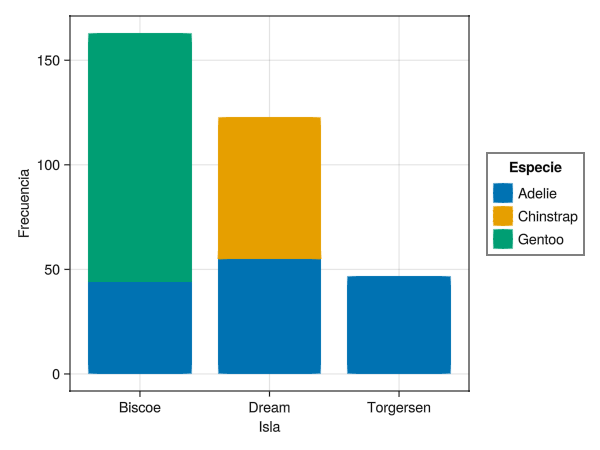
\includegraphics[keepaspectratio]{07-arboles-decision_files/figure-pdf/cell-12-output-1.png}}

\begin{Shaded}
\begin{Highlighting}[]
\NormalTok{frec\_sexo }\OperatorTok{=} \FunctionTok{combine}\NormalTok{(}\FunctionTok{groupby}\NormalTok{(df, [}\OperatorTok{:}\NormalTok{Sexo, }\OperatorTok{:}\NormalTok{Especie]), nrow }\OperatorTok{=\textgreater{}} \OperatorTok{:}\NormalTok{Frecuencia)}
\FunctionTok{data}\NormalTok{(frec\_sexo) }\OperatorTok{*} 
    \FunctionTok{mapping}\NormalTok{(}\OperatorTok{:}\NormalTok{Sexo, }\OperatorTok{:}\NormalTok{Frecuencia, stack }\OperatorTok{=} \OperatorTok{:}\NormalTok{Especie, color }\OperatorTok{=:}\NormalTok{Especie) }\OperatorTok{*}
    \FunctionTok{visual}\NormalTok{(BarPlot) }\OperatorTok{|\textgreater{}}\NormalTok{ draw}
\end{Highlighting}
\end{Shaded}

  \pandocbounded{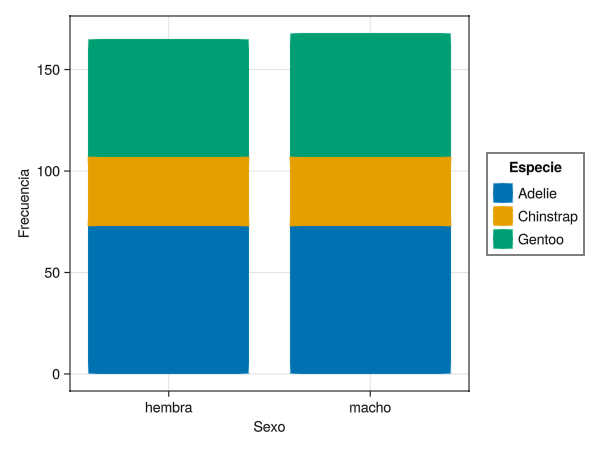
\includegraphics[keepaspectratio]{07-arboles-decision_files/figure-pdf/cell-13-output-1.png}}

  Para las variables cuantitativas dibujamos diagramas de cajas.

\begin{Shaded}
\begin{Highlighting}[]
\KeywordTok{function} \FunctionTok{cajas}\NormalTok{(df, var, clase)}
    \FunctionTok{data}\NormalTok{(df) }\OperatorTok{*}
        \FunctionTok{mapping}\NormalTok{(clase, var, color }\OperatorTok{=}\NormalTok{ clase) }\OperatorTok{*}
        \FunctionTok{visual}\NormalTok{(BoxPlot) }\OperatorTok{|\textgreater{}} 
\NormalTok{        draw}
\KeywordTok{end}

\FunctionTok{cajas}\NormalTok{(df, }\OperatorTok{:}\NormalTok{Longitud\_pico, }\OperatorTok{:}\NormalTok{Especie)}
\end{Highlighting}
\end{Shaded}

  \pandocbounded{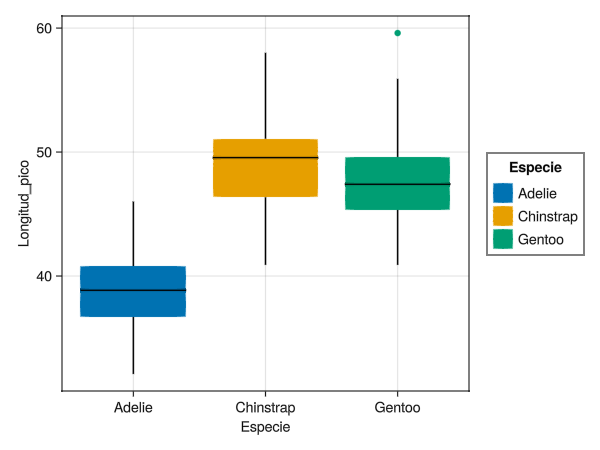
\includegraphics[keepaspectratio]{07-arboles-decision_files/figure-pdf/cell-14-output-1.png}}

\begin{Shaded}
\begin{Highlighting}[]
\FunctionTok{cajas}\NormalTok{(df, }\OperatorTok{:}\NormalTok{Profundidad\_pico, }\OperatorTok{:}\NormalTok{Especie)}
\end{Highlighting}
\end{Shaded}

  \pandocbounded{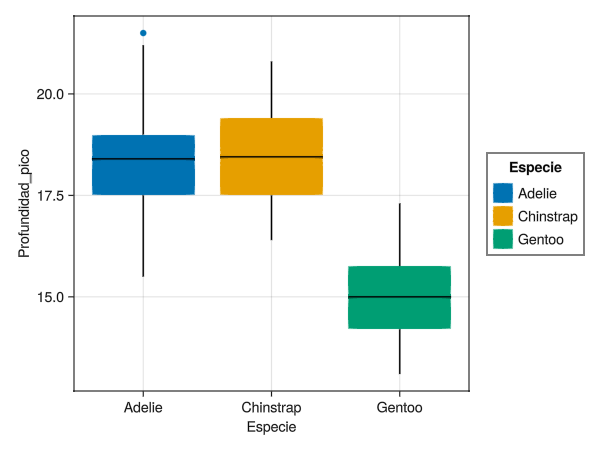
\includegraphics[keepaspectratio]{07-arboles-decision_files/figure-pdf/cell-15-output-1.png}}

\begin{Shaded}
\begin{Highlighting}[]
\FunctionTok{cajas}\NormalTok{(df, }\OperatorTok{:}\NormalTok{Longitud\_ala, }\OperatorTok{:}\NormalTok{Especie)}
\end{Highlighting}
\end{Shaded}

  \pandocbounded{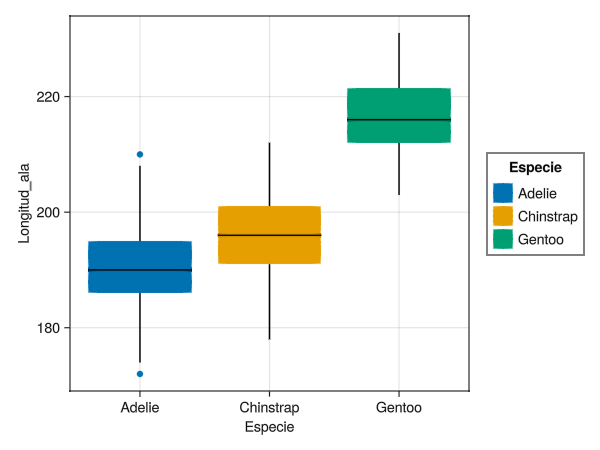
\includegraphics[keepaspectratio]{07-arboles-decision_files/figure-pdf/cell-16-output-1.png}}

\begin{Shaded}
\begin{Highlighting}[]
\FunctionTok{cajas}\NormalTok{(df, }\OperatorTok{:}\NormalTok{Peso, }\OperatorTok{:}\NormalTok{Especie)}
\end{Highlighting}
\end{Shaded}

  \pandocbounded{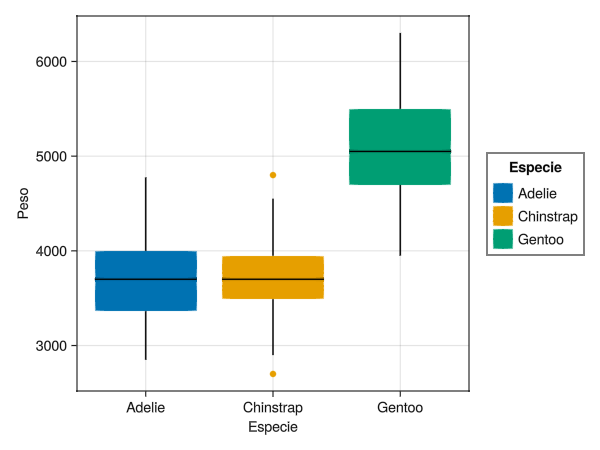
\includegraphics[keepaspectratio]{07-arboles-decision_files/figure-pdf/cell-17-output-1.png}}

  \end{tcolorbox}
\item
  ¿Cuál es la reducción de la impureza del conjunto de datos si
  dividimos el conjunto de datos en dos conjuntos según si la longitud
  del pico es mayor o menor que 44 mm?

  \begin{tcolorbox}[enhanced jigsaw, toptitle=1mm, colframe=quarto-callout-tip-color-frame, titlerule=0mm, left=2mm, arc=.35mm, colbacktitle=quarto-callout-tip-color!10!white, opacityback=0, bottomtitle=1mm, toprule=.15mm, coltitle=black, breakable, colback=white, rightrule=.15mm, opacitybacktitle=0.6, leftrule=.75mm, bottomrule=.15mm, title=\textcolor{quarto-callout-tip-color}{\faLightbulb}\hspace{0.5em}{Solución}]

\begin{Shaded}
\begin{Highlighting}[]
\ImportTok{using} \BuiltInTok{Tidier}
\KeywordTok{function} \FunctionTok{gini}\NormalTok{(df}\OperatorTok{::}\DataTypeTok{DataFrame}\NormalTok{, var}\OperatorTok{::}\DataTypeTok{Symbol}\NormalTok{)}
\NormalTok{    n }\OperatorTok{=} \FunctionTok{nrow}\NormalTok{(df)}
\NormalTok{    frec }\OperatorTok{=} \FunctionTok{combine}\NormalTok{(}\FunctionTok{groupby}\NormalTok{(df, var), nrow }\OperatorTok{=\textgreater{}} \OperatorTok{:}\NormalTok{ni)}
\NormalTok{    frec.p }\OperatorTok{=}\NormalTok{ frec.ni }\OperatorTok{./}\NormalTok{ n}
\NormalTok{    gini }\OperatorTok{=} \FloatTok{1} \OperatorTok{{-}} \FunctionTok{sum}\NormalTok{(frec.p }\OperatorTok{.\^{}} \FloatTok{2}\NormalTok{)}
    \ControlFlowTok{return}\NormalTok{ gini}
\KeywordTok{end}

\KeywordTok{function} \FunctionTok{reduccion\_impureza}\NormalTok{(df}\OperatorTok{::}\DataTypeTok{DataFrame}\NormalTok{, var}\OperatorTok{::}\DataTypeTok{Symbol}\NormalTok{, val}\OperatorTok{::}\DataTypeTok{Number}\NormalTok{)}
    \CommentTok{\# Dividimos el conjunto de ejemplos según la longitud del pico es menor de 44.}
\NormalTok{    df\_menor }\OperatorTok{=} \PreprocessorTok{@eval} \PreprocessorTok{@filter}\NormalTok{(}\OperatorTok{$}\NormalTok{df, }\OperatorTok{$}\NormalTok{var }\OperatorTok{\textless{}=} \OperatorTok{$}\NormalTok{val)}
\NormalTok{    df\_mayor }\OperatorTok{=} \PreprocessorTok{@eval} \PreprocessorTok{@filter}\NormalTok{(}\OperatorTok{$}\NormalTok{df, }\OperatorTok{$}\NormalTok{var }\OperatorTok{\textgreater{}} \OperatorTok{$}\NormalTok{val)}
    \CommentTok{\# Calculamos los tamaños de los subconjuntos de ejemplos.}
\NormalTok{    n }\OperatorTok{=} \FunctionTok{nrow}\NormalTok{(df\_menor), }\FunctionTok{nrow}\NormalTok{(df\_mayor)}
    \CommentTok{\# Calculamos el índice de Gini de cada subconjunto.}
\NormalTok{    gis }\OperatorTok{=} \FunctionTok{gini}\NormalTok{(df\_menor, }\OperatorTok{:}\NormalTok{Especie), }\FunctionTok{gini}\NormalTok{(df\_mayor, }\OperatorTok{:}\NormalTok{Especie)}
    \CommentTok{\# Calculamos media ponderada de los índices de Gini de los subconjuntos.}
\NormalTok{    g1 }\OperatorTok{=} \FunctionTok{sum}\NormalTok{(gis }\OperatorTok{.*}\NormalTok{ n) }\OperatorTok{/} \FunctionTok{sum}\NormalTok{(n)}
    \CommentTok{\# Calculamos la reducción del índice de Gini.}
    \FunctionTok{gini}\NormalTok{(df, }\OperatorTok{:}\NormalTok{Especie) }\OperatorTok{{-}}\NormalTok{ g1}
\KeywordTok{end}

\FunctionTok{reduccion\_impureza}\NormalTok{(df, }\OperatorTok{:}\NormalTok{Longitud\_pico, }\FloatTok{44}\NormalTok{)}
\end{Highlighting}
\end{Shaded}

\begin{verbatim}
0.26577182779353914
\end{verbatim}

  \end{tcolorbox}
\item
  Determinar el valor óptimo de división del conjunto de datos según la
  longitud del pico. Para ello, calcular la reducción de la impureza
  para cada valor de longitud del pico y dibujar el resultado.

  \begin{tcolorbox}[enhanced jigsaw, toptitle=1mm, colframe=quarto-callout-tip-color-frame, titlerule=0mm, left=2mm, arc=.35mm, colbacktitle=quarto-callout-tip-color!10!white, opacityback=0, bottomtitle=1mm, toprule=.15mm, coltitle=black, breakable, colback=white, rightrule=.15mm, opacitybacktitle=0.6, leftrule=.75mm, bottomrule=.15mm, title=\textcolor{quarto-callout-tip-color}{\faLightbulb}\hspace{0.5em}{Solución}]

  Dibujamos la reducción de la impureza en función de la longitud del
  pico.

\begin{Shaded}
\begin{Highlighting}[]
\ImportTok{using} \BuiltInTok{Plots}
\CommentTok{\# Valores únicos de longitud del pico.}
\NormalTok{valores }\OperatorTok{=} \FunctionTok{unique}\NormalTok{(df.Longitud\_pico)}
\CommentTok{\# Reducción de la impureza para cada valor.}
\NormalTok{reducciones }\OperatorTok{=}\NormalTok{ [}\FunctionTok{reduccion\_impureza}\NormalTok{(df, }\OperatorTok{:}\NormalTok{Longitud\_pico, val) for val }\KeywordTok{in}\NormalTok{ valores]}
\CommentTok{\# Graficamos el resultado.}
\NormalTok{Plots.}\FunctionTok{scatter}\NormalTok{(valores, reducciones, xlabel }\OperatorTok{=} \StringTok{"Longitud del pico"}\NormalTok{, ylabel }\OperatorTok{=} \StringTok{"Reducción de la impureza"}\NormalTok{, legend }\OperatorTok{=} \ConstantTok{false}\NormalTok{)}
\end{Highlighting}
\end{Shaded}

  \pandocbounded{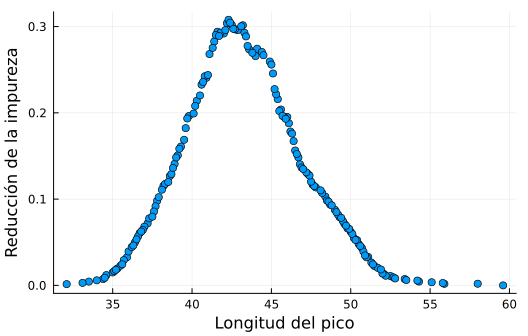
\includegraphics[keepaspectratio]{index_files/mediabag/07-arboles-decision_files/figure-pdf/cell-19-output-1.pdf}}

  Y ahora obtenemos el valor óptimo de división del conjunto de datos
  según la longitud del pico.

\begin{Shaded}
\begin{Highlighting}[]
\NormalTok{val\_optimo }\OperatorTok{=}\NormalTok{ valores[}\FunctionTok{argmax}\NormalTok{(reducciones)]}
\end{Highlighting}
\end{Shaded}

\begin{verbatim}
42.3
\end{verbatim}

  \end{tcolorbox}
\item
  Dividir aleatoriamente el dataframe en un conjunto de entrenamiento y
  un conjunto de test con proporciones \(3/4\) y \(1/4\)
  respectivamente.

  \begin{tcolorbox}[enhanced jigsaw, toptitle=1mm, colframe=quarto-callout-note-color-frame, titlerule=0mm, left=2mm, arc=.35mm, colbacktitle=quarto-callout-note-color!10!white, opacityback=0, bottomtitle=1mm, toprule=.15mm, coltitle=black, breakable, colback=white, rightrule=.15mm, opacitybacktitle=0.6, leftrule=.75mm, bottomrule=.15mm, title=\textcolor{quarto-callout-note-color}{\faInfo}\hspace{0.5em}{Ayuda}]

  Utilizar la función
  \href{https://docs.julialang.org/en/v1/stdlib/Random/\#Random.shuffle}{\texttt{shuffle}}
  del paquete
  \href{https://docs.julialang.org/en/v1/stdlib/Random/}{\texttt{Random}}
  para barajar el dataframe y luego dividirlo en dos subconjuntos.

  \end{tcolorbox}

  \begin{tcolorbox}[enhanced jigsaw, toptitle=1mm, colframe=quarto-callout-tip-color-frame, titlerule=0mm, left=2mm, arc=.35mm, colbacktitle=quarto-callout-tip-color!10!white, opacityback=0, bottomtitle=1mm, toprule=.15mm, coltitle=black, breakable, colback=white, rightrule=.15mm, opacitybacktitle=0.6, leftrule=.75mm, bottomrule=.15mm, title=\textcolor{quarto-callout-tip-color}{\faLightbulb}\hspace{0.5em}{Solución}]

\begin{Shaded}
\begin{Highlighting}[]
\ImportTok{using} \BuiltInTok{Random}
\CommentTok{\# Establecemos la semilla para la reproducibilidad.}
\BuiltInTok{Random}\NormalTok{.}\FunctionTok{seed!}\NormalTok{(}\FloatTok{1234}\NormalTok{)}
\CommentTok{\# Barajamos el dataframe.}
\NormalTok{df }\OperatorTok{=} \FunctionTok{shuffle}\NormalTok{(df)}
\CommentTok{\# Dividimos el dataframe en un conjunto de entrenamiento y un conjunto de test.}
\NormalTok{n }\OperatorTok{=} \FunctionTok{nrow}\NormalTok{(df)}
\NormalTok{df\_test }\OperatorTok{=}\NormalTok{ df[}\FloatTok{1}\OperatorTok{:}\FunctionTok{div}\NormalTok{(n, }\FloatTok{4}\NormalTok{), }\OperatorTok{:}\NormalTok{]}
\NormalTok{df\_train }\OperatorTok{=}\NormalTok{ df[}\FunctionTok{div}\NormalTok{(n, }\FloatTok{4}\NormalTok{)}\OperatorTok{+}\FloatTok{1}\OperatorTok{:}\KeywordTok{end}\NormalTok{, }\OperatorTok{:}\NormalTok{]}
\end{Highlighting}
\end{Shaded}

  \begin{tabular}{r|ccccccc}
      & Especie & Isla & Longitud\_pico & Profundidad\_pico & Longitud\_ala & Peso & Sexo\\
      \hline
      & String15 & String15 & Float64 & Float64 & Int64 & Int64 & String7\\
      \hline
      1 & Adelie & Dream & 39.0 & 18.7 & 185 & 3650 & macho \\
      2 & Chinstrap & Dream & 52.8 & 20.0 & 205 & 4550 & macho \\
      3 & Chinstrap & Dream & 55.8 & 19.8 & 207 & 4000 & macho \\
      4 & Adelie & Torgersen & 35.1 & 19.4 & 193 & 4200 & macho \\
      5 & Adelie & Torgersen & 34.6 & 21.1 & 198 & 4400 & macho \\
      6 & Gentoo & Biscoe & 50.0 & 15.2 & 218 & 5700 & macho \\
      7 & Chinstrap & Dream & 50.6 & 19.4 & 193 & 3800 & macho \\
      8 & Chinstrap & Dream & 43.5 & 18.1 & 202 & 3400 & hembra \\
      9 & Adelie & Dream & 36.9 & 18.6 & 189 & 3500 & hembra \\
      10 & Adelie & Dream & 36.6 & 18.4 & 184 & 3475 & hembra \\
      11 & Chinstrap & Dream & 46.6 & 17.8 & 193 & 3800 & hembra \\
      12 & Gentoo & Biscoe & 50.8 & 17.3 & 228 & 5600 & macho \\
      13 & Chinstrap & Dream & 52.2 & 18.8 & 197 & 3450 & macho \\
      14 & Adelie & Dream & 39.6 & 18.8 & 190 & 4600 & macho \\
      15 & Adelie & Torgersen & 42.8 & 18.5 & 195 & 4250 & macho \\
      16 & Adelie & Biscoe & 36.5 & 16.6 & 181 & 2850 & hembra \\
      17 & Gentoo & Biscoe & 49.1 & 14.8 & 220 & 5150 & hembra \\
      18 & Chinstrap & Dream & 43.2 & 16.6 & 187 & 2900 & hembra \\
      19 & Gentoo & Biscoe & 43.3 & 13.4 & 209 & 4400 & hembra \\
      20 & Gentoo & Biscoe & 49.5 & 16.1 & 224 & 5650 & macho \\
      21 & Adelie & Biscoe & 37.8 & 20.0 & 190 & 4250 & macho \\
      22 & Gentoo & Biscoe & 50.4 & 15.3 & 224 & 5550 & macho \\
      23 & Adelie & Biscoe & 45.6 & 20.3 & 191 & 4600 & macho \\
      24 & Chinstrap & Dream & 45.4 & 18.7 & 188 & 3525 & hembra \\
      25 & Adelie & Dream & 39.2 & 18.6 & 190 & 4250 & macho \\
      26 & Gentoo & Biscoe & 48.4 & 14.4 & 203 & 4625 & hembra \\
      27 & Adelie & Torgersen & 35.2 & 15.9 & 186 & 3050 & hembra \\
      28 & Gentoo & Biscoe & 48.4 & 16.3 & 220 & 5400 & macho \\
      29 & Adelie & Dream & 33.1 & 16.1 & 178 & 2900 & hembra \\
      30 & Adelie & Dream & 36.8 & 18.5 & 193 & 3500 & hembra \\
      $\dots$ & $\dots$ & $\dots$ & $\dots$ & $\dots$ & $\dots$ & $\dots$ & $\dots$ \\
  \end{tabular}

  \end{tcolorbox}
\item
  Construir un árbol de decisión con el conjunto de entrenamiento sin
  tener en cuenta la variable \texttt{Isla} y visualizarlo.

  \begin{tcolorbox}[enhanced jigsaw, toptitle=1mm, colframe=quarto-callout-tip-color-frame, titlerule=0mm, left=2mm, arc=.35mm, colbacktitle=quarto-callout-tip-color!10!white, opacityback=0, bottomtitle=1mm, toprule=.15mm, coltitle=black, breakable, colback=white, rightrule=.15mm, opacitybacktitle=0.6, leftrule=.75mm, bottomrule=.15mm, title=\textcolor{quarto-callout-tip-color}{\faLightbulb}\hspace{0.5em}{Solución}]

\begin{Shaded}
\begin{Highlighting}[]
\ImportTok{using} \BuiltInTok{DecisionTree}\NormalTok{, }\BuiltInTok{CategoricalArrays}
\CommentTok{\# Variables predictivas.}
\NormalTok{X\_train }\OperatorTok{=} \FunctionTok{Matrix}\NormalTok{(}\FunctionTok{select}\NormalTok{(df\_train, }\FunctionTok{Not}\NormalTok{(}\OperatorTok{:}\NormalTok{Isla, }\OperatorTok{:}\NormalTok{Especie)))}
\CommentTok{\# Variable objetivo.}
\NormalTok{y\_train }\OperatorTok{=}\NormalTok{ df\_train.Especie}
\CommentTok{\# Convertir las variables categóricas a enteros.}
\NormalTok{X\_train }\OperatorTok{=} \FunctionTok{hcat}\NormalTok{([}\FunctionTok{levelcode}\NormalTok{.(}\FunctionTok{categorical}\NormalTok{(X\_train[}\OperatorTok{:}\NormalTok{, j])) for j }\KeywordTok{in} \FloatTok{1}\OperatorTok{:}\FunctionTok{size}\NormalTok{(X\_train, }\FloatTok{2}\NormalTok{)]}\OperatorTok{...}\NormalTok{)}
\CommentTok{\# Convertir la variable objetivo a enteros}
\NormalTok{y\_train }\OperatorTok{=} \FunctionTok{levelcode}\NormalTok{.(}\FunctionTok{categorical}\NormalTok{(y\_train))}

\CommentTok{\# Construimos el árbol de decisión con profundidad máxima 3.}
\NormalTok{tree }\OperatorTok{=} \FunctionTok{DecisionTreeClassifier}\NormalTok{(max\_depth }\OperatorTok{=} \FloatTok{3}\NormalTok{)}
\FunctionTok{fit!}\NormalTok{(tree, X\_train, y\_train)}
\FunctionTok{print\_tree}\NormalTok{(tree, feature\_names}\OperatorTok{=}\FunctionTok{names}\NormalTok{(df)[}\FloatTok{3}\OperatorTok{:}\KeywordTok{end}\NormalTok{])}
\end{Highlighting}
\end{Shaded}

\begin{verbatim}
Feature 3: "Longitud_ala" < 29.0 ?
├─ Feature 1: "Longitud_pico" < 62.0 ?
    ├─ 1 : 96/96
    └─ Feature 1: "Longitud_pico" < 87.0 ?
        ├─ 2 : 10/20
        └─ 2 : 37/38
└─ Feature 2: "Profundidad_pico" < 46.0 ?
    ├─ 3 : 90/90
    └─ Feature 1: "Longitud_pico" < 109.0 ?
        ├─ 1 : 2/2
        └─ 2 : 4/4
\end{verbatim}

  \end{tcolorbox}
\item
  Predecir la especie de los pingüinos del conjunto de test y calcular
  la matriz de confusión de las predicciones.

  \begin{tcolorbox}[enhanced jigsaw, toptitle=1mm, colframe=quarto-callout-note-color-frame, titlerule=0mm, left=2mm, arc=.35mm, colbacktitle=quarto-callout-note-color!10!white, opacityback=0, bottomtitle=1mm, toprule=.15mm, coltitle=black, breakable, colback=white, rightrule=.15mm, opacitybacktitle=0.6, leftrule=.75mm, bottomrule=.15mm, title=\textcolor{quarto-callout-note-color}{\faInfo}\hspace{0.5em}{Ayuda}]

  Utilizar la función
  \href{https://juliaai.github.io/StatisticalMeasures.jl/stable/confusion_matrices/\#StatisticalMeasures.ConfusionMatrices.confmat}{\texttt{confmat}}
  del paquete
  \href{https://juliaai.github.io/StatisticalMeasures.jl}{\texttt{StatisticalMeaures}}
  para barajar el dataframe y luego dividirlo en dos subconjuntos.

  \end{tcolorbox}

  \begin{tcolorbox}[enhanced jigsaw, toptitle=1mm, colframe=quarto-callout-tip-color-frame, titlerule=0mm, left=2mm, arc=.35mm, colbacktitle=quarto-callout-tip-color!10!white, opacityback=0, bottomtitle=1mm, toprule=.15mm, coltitle=black, breakable, colback=white, rightrule=.15mm, opacitybacktitle=0.6, leftrule=.75mm, bottomrule=.15mm, title=\textcolor{quarto-callout-tip-color}{\faLightbulb}\hspace{0.5em}{Solución}]

\begin{Shaded}
\begin{Highlighting}[]
\ImportTok{using} \BuiltInTok{StatisticalMeasures}
\CommentTok{\# Variables predictivas}
\NormalTok{X\_test }\OperatorTok{=} \FunctionTok{Matrix}\NormalTok{(}\FunctionTok{select}\NormalTok{(df\_test, }\FunctionTok{Not}\NormalTok{(}\OperatorTok{:}\NormalTok{Isla, }\OperatorTok{:}\NormalTok{Especie)))}
\CommentTok{\# Variable objetivo}
\NormalTok{y\_test }\OperatorTok{=}\NormalTok{ df\_test.Especie}
\CommentTok{\# Convertir las variables categóricas a enteros}
\NormalTok{X\_test }\OperatorTok{=} \FunctionTok{hcat}\NormalTok{([}\FunctionTok{levelcode}\NormalTok{.(}\FunctionTok{categorical}\NormalTok{(X\_test[}\OperatorTok{:}\NormalTok{, j])) for j }\KeywordTok{in} \FloatTok{1}\OperatorTok{:}\FunctionTok{size}\NormalTok{(X\_test, }\FloatTok{2}\NormalTok{)]}\OperatorTok{...}\NormalTok{)}
\CommentTok{\# Convertir la variable objetivo a enteros}
\NormalTok{y\_test }\OperatorTok{=} \FunctionTok{levelcode}\NormalTok{.(}\FunctionTok{categorical}\NormalTok{(y\_test))}
\CommentTok{\# Predecimos la especie de pingüino del conjunto de test}
\NormalTok{y\_pred }\OperatorTok{=} \FunctionTok{predict}\NormalTok{(tree, X\_test)}
\CommentTok{\# Calculamos la precisión del modelo}
\FunctionTok{confmat}\NormalTok{(y\_pred, y\_test)}
\end{Highlighting}
\end{Shaded}

\begin{verbatim}
          ┌──────────────┐
          │ Ground Truth │
┌─────────┼────┬────┬────┤
│Predicted│ 1  │ 2  │ 3  │
├─────────┼────┼────┼────┤
│    1    │ 38 │ 11 │ 9  │
├─────────┼────┼────┼────┤
│    2    │ 0  │ 6  │ 0  │
├─────────┼────┼────┼────┤
│    3    │ 0  │ 0  │ 19 │
└─────────┴────┴────┴────┘
\end{verbatim}

  \end{tcolorbox}
\item
  Calcular la precisión del modelo.

  \begin{tcolorbox}[enhanced jigsaw, toptitle=1mm, colframe=quarto-callout-note-color-frame, titlerule=0mm, left=2mm, arc=.35mm, colbacktitle=quarto-callout-note-color!10!white, opacityback=0, bottomtitle=1mm, toprule=.15mm, coltitle=black, breakable, colback=white, rightrule=.15mm, opacitybacktitle=0.6, leftrule=.75mm, bottomrule=.15mm, title=\textcolor{quarto-callout-note-color}{\faInfo}\hspace{0.5em}{Ayuda}]

  La precisión es la proporción de predicciones correctas sobre el total
  de predicciones.

  Utilizar la función
  \href{https://juliaai.github.io/StatisticalMeasures.jl/stable/auto_generated_list_of_measures/\#StatisticalMeasures.Accuracy}{\texttt{accuracy}}
  del paquete
  \href{https://juliaai.github.io/StatisticalMeasures.jl}{\texttt{StatisticalMeaures}}
  para calcular la precisión del modelo.

  \end{tcolorbox}

  \begin{tcolorbox}[enhanced jigsaw, toptitle=1mm, colframe=quarto-callout-tip-color-frame, titlerule=0mm, left=2mm, arc=.35mm, colbacktitle=quarto-callout-tip-color!10!white, opacityback=0, bottomtitle=1mm, toprule=.15mm, coltitle=black, breakable, colback=white, rightrule=.15mm, opacitybacktitle=0.6, leftrule=.75mm, bottomrule=.15mm, title=\textcolor{quarto-callout-tip-color}{\faLightbulb}\hspace{0.5em}{Solución}]

\begin{Shaded}
\begin{Highlighting}[]
\CommentTok{\# Calculamos la precisión del modelo}
\FunctionTok{accuracy}\NormalTok{(y\_pred, y\_test)}
\end{Highlighting}
\end{Shaded}

\begin{verbatim}
0.7590361445783133
\end{verbatim}

  \end{tcolorbox}
\end{enumerate}

\end{exercise}

\begin{exercise}[]\protect\hypertarget{exr-arboles-decision-3}{}\label{exr-arboles-decision-3}

El fichero \href{datos/vinos.csv}{\texttt{vinos.csv}} contiene
información sobre las características de una muestra de vinos
portugueses de la denominación ``Vinho Verde''. Las variables que
contiene son:

\begin{longtable}[]{@{}
  >{\raggedright\arraybackslash}p{(\linewidth - 4\tabcolsep) * \real{0.2963}}
  >{\raggedright\arraybackslash}p{(\linewidth - 4\tabcolsep) * \real{0.5259}}
  >{\raggedright\arraybackslash}p{(\linewidth - 4\tabcolsep) * \real{0.1778}}@{}}
\toprule\noalign{}
\begin{minipage}[b]{\linewidth}\raggedright
Variable
\end{minipage} & \begin{minipage}[b]{\linewidth}\raggedright
Descripción
\end{minipage} & \begin{minipage}[b]{\linewidth}\raggedright
Tipo (unidades)
\end{minipage} \\
\midrule\noalign{}
\endhead
\bottomrule\noalign{}
\endlastfoot
tipo & Tipo de vino & Categórica (blanco, tinto) \\
meses.barrica & Mesesde envejecimiento en barrica & Numérica(meses) \\
acided.fija & Cantidadde ácidotartárico & Numérica(g/dm3) \\
acided.volatil & Cantidad de ácido acético & Numérica(g/dm3) \\
acido.citrico & Cantidad de ácidocítrico & Numérica(g/dm3) \\
azucar.residual & Cantidad de azúcarremanente después de la fermentación
& Numérica(g/dm3) \\
cloruro.sodico & Cantidad de clorurosódico & Numérica(g/dm3) \\
dioxido.azufre.libre & Cantidad de dióxido de azufreen formalibre &
Numérica(mg/dm3) \\
dioxido.azufre.total & Cantidadde dióxido de azufretotal en forma libre
o ligada & Numérica(mg/dm3) \\
densidad & Densidad & Numérica(g/cm3) \\
ph & pH & Numérica(0-14) \\
sulfatos & Cantidadde sulfato de potasio & Numérica(g/dm3) \\
alcohol & Porcentajede contenidode alcohol & Numérica(0-100) \\
calidad & Calificación otorgada porun panel de expertos &
Numérica(0-10) \\
\end{longtable}

\begin{enumerate}
\def\labelenumi{\alph{enumi}.}
\item
  Crear un data frame con los datos de los vinos a partir del fichero
  \href{datos/vinos.csv}{\texttt{vinos.csv}}.

  \begin{tcolorbox}[enhanced jigsaw, toptitle=1mm, colframe=quarto-callout-tip-color-frame, titlerule=0mm, left=2mm, arc=.35mm, colbacktitle=quarto-callout-tip-color!10!white, opacityback=0, bottomtitle=1mm, toprule=.15mm, coltitle=black, breakable, colback=white, rightrule=.15mm, opacitybacktitle=0.6, leftrule=.75mm, bottomrule=.15mm, title=\textcolor{quarto-callout-tip-color}{\faLightbulb}\hspace{0.5em}{Solución}]

\begin{Shaded}
\begin{Highlighting}[]
\ImportTok{using} \BuiltInTok{CSV}\NormalTok{, }\BuiltInTok{DataFrames}
\NormalTok{df }\OperatorTok{=}\NormalTok{ CSV.}\FunctionTok{read}\NormalTok{(}\StringTok{"datos/vinos.csv"}\NormalTok{, DataFrame)}
\end{Highlighting}
\end{Shaded}

  \begin{tabular}{r|ccccccc}
      & tipo & meses\_barrica & acided\_fija & acided\_volatil & acido\_citrico & azucar\_residual & \\
      \hline
      & String7 & Int64 & Float64 & Float64 & Float64 & Float64 & \\
      \hline
      1 & blanco & 0 & 7.0 & 0.27 & 0.36 & 20.7 & $\dots$ \\
      2 & blanco & 0 & 6.3 & 0.3 & 0.34 & 1.6 & $\dots$ \\
      3 & blanco & 0 & 8.1 & 0.28 & 0.4 & 6.9 & $\dots$ \\
      4 & blanco & 0 & 7.2 & 0.23 & 0.32 & 8.5 & $\dots$ \\
      5 & blanco & 0 & 6.2 & 0.32 & 0.16 & 7.0 & $\dots$ \\
      6 & blanco & 0 & 8.1 & 0.22 & 0.43 & 1.5 & $\dots$ \\
      7 & blanco & 0 & 8.1 & 0.27 & 0.41 & 1.45 & $\dots$ \\
      8 & blanco & 0 & 8.6 & 0.23 & 0.4 & 4.2 & $\dots$ \\
      9 & blanco & 0 & 7.9 & 0.18 & 0.37 & 1.2 & $\dots$ \\
      10 & blanco & 0 & 6.6 & 0.16 & 0.4 & 1.5 & $\dots$ \\
      11 & blanco & 0 & 8.3 & 0.42 & 0.62 & 19.25 & $\dots$ \\
      12 & blanco & 0 & 6.6 & 0.17 & 0.38 & 1.5 & $\dots$ \\
      13 & blanco & 0 & 6.3 & 0.48 & 0.04 & 1.1 & $\dots$ \\
      14 & blanco & 0 & 6.2 & 0.66 & 0.48 & 1.2 & $\dots$ \\
      15 & blanco & 0 & 7.4 & 0.34 & 0.42 & 1.1 & $\dots$ \\
      16 & blanco & 0 & 6.5 & 0.31 & 0.14 & 7.5 & $\dots$ \\
      17 & blanco & 0 & 6.4 & 0.31 & 0.38 & 2.9 & $\dots$ \\
      18 & blanco & 0 & 6.8 & 0.26 & 0.42 & 1.7 & $\dots$ \\
      19 & blanco & 0 & 7.6 & 0.67 & 0.14 & 1.5 & $\dots$ \\
      20 & blanco & 0 & 6.6 & 0.27 & 0.41 & 1.3 & $\dots$ \\
      21 & blanco & 0 & 7.0 & 0.25 & 0.32 & 9.0 & $\dots$ \\
      22 & blanco & 0 & 6.9 & 0.24 & 0.35 & 1.0 & $\dots$ \\
      23 & blanco & 0 & 7.0 & 0.28 & 0.39 & 8.7 & $\dots$ \\
      24 & blanco & 0 & 7.4 & 0.27 & 0.48 & 1.1 & $\dots$ \\
      25 & blanco & 0 & 7.2 & 0.32 & 0.36 & 2.0 & $\dots$ \\
      26 & blanco & 0 & 8.5 & 0.24 & 0.39 & 10.4 & $\dots$ \\
      27 & blanco & 0 & 8.3 & 0.14 & 0.34 & 1.1 & $\dots$ \\
      28 & blanco & 0 & 7.4 & 0.25 & 0.36 & 2.05 & $\dots$ \\
      29 & blanco & 0 & 6.2 & 0.12 & 0.34 & 1.5 & $\dots$ \\
      30 & blanco & 0 & 5.8 & 0.27 & 0.2 & 14.95 & $\dots$ \\
      $\dots$ & $\dots$ & $\dots$ & $\dots$ & $\dots$ & $\dots$ & $\dots$ &  \\
  \end{tabular}

  \end{tcolorbox}
\item
  Mostrar los tipos de cada variable del data frame.

  \begin{tcolorbox}[enhanced jigsaw, toptitle=1mm, colframe=quarto-callout-note-color-frame, titlerule=0mm, left=2mm, arc=.35mm, colbacktitle=quarto-callout-note-color!10!white, opacityback=0, bottomtitle=1mm, toprule=.15mm, coltitle=black, breakable, colback=white, rightrule=.15mm, opacitybacktitle=0.6, leftrule=.75mm, bottomrule=.15mm, title=\textcolor{quarto-callout-note-color}{\faInfo}\hspace{0.5em}{Ayuda}]

  Usar la función \texttt{schema} del paquete
  \href{https://juliaai.github.io/MLJ.jl/}{\texttt{MLJ}}.

  \end{tcolorbox}

  \begin{tcolorbox}[enhanced jigsaw, toptitle=1mm, colframe=quarto-callout-tip-color-frame, titlerule=0mm, left=2mm, arc=.35mm, colbacktitle=quarto-callout-tip-color!10!white, opacityback=0, bottomtitle=1mm, toprule=.15mm, coltitle=black, breakable, colback=white, rightrule=.15mm, opacitybacktitle=0.6, leftrule=.75mm, bottomrule=.15mm, title=\textcolor{quarto-callout-tip-color}{\faLightbulb}\hspace{0.5em}{Solución}]

\begin{Shaded}
\begin{Highlighting}[]
\ImportTok{using} \BuiltInTok{MLJ}
\FunctionTok{schema}\NormalTok{(df)}
\end{Highlighting}
\end{Shaded}

\begin{verbatim}
WARNING: using MLJ.fit! in module Main conflicts with an existing identifier.
WARNING: using MLJ.predict in module Main conflicts with an existing identifier.
\end{verbatim}

\begin{verbatim}
┌──────────────────────┬────────────┬─────────┐
│ names                │ scitypes   │ types   │
├──────────────────────┼────────────┼─────────┤
│ tipo                 │ Textual    │ String7 │
│ meses_barrica        │ Count      │ Int64   │
│ acided_fija          │ Continuous │ Float64 │
│ acided_volatil       │ Continuous │ Float64 │
│ acido_citrico        │ Continuous │ Float64 │
│ azucar_residual      │ Continuous │ Float64 │
│ cloruro_sodico       │ Continuous │ Float64 │
│ dioxido_azufre_libre │ Continuous │ Float64 │
│ dioxido_azufre_total │ Continuous │ Float64 │
│ densidad             │ Continuous │ Float64 │
│ ph                   │ Continuous │ Float64 │
│ sulfatos             │ Continuous │ Float64 │
│ alcohol              │ Continuous │ Float64 │
│ calidad              │ Count      │ Int64   │
└──────────────────────┴────────────┴─────────┘
\end{verbatim}

  \end{tcolorbox}
\item
  Hacer un análisis de los datos perdidos en el data frame.

  \begin{tcolorbox}[enhanced jigsaw, toptitle=1mm, colframe=quarto-callout-tip-color-frame, titlerule=0mm, left=2mm, arc=.35mm, colbacktitle=quarto-callout-tip-color!10!white, opacityback=0, bottomtitle=1mm, toprule=.15mm, coltitle=black, breakable, colback=white, rightrule=.15mm, opacitybacktitle=0.6, leftrule=.75mm, bottomrule=.15mm, title=\textcolor{quarto-callout-tip-color}{\faLightbulb}\hspace{0.5em}{Solución}]

\begin{Shaded}
\begin{Highlighting}[]
\FunctionTok{describe}\NormalTok{(df, }\OperatorTok{:}\NormalTok{nmissing)}
\end{Highlighting}
\end{Shaded}

  \begin{tabular}{r|cc}
      & variable & nmissing\\
      \hline
      & Symbol & Int64\\
      \hline
      1 & tipo & 0 \\
      2 & meses\_barrica & 0 \\
      3 & acided\_fija & 0 \\
      4 & acided\_volatil & 0 \\
      5 & acido\_citrico & 0 \\
      6 & azucar\_residual & 0 \\
      7 & cloruro\_sodico & 0 \\
      8 & dioxido\_azufre\_libre & 0 \\
      9 & dioxido\_azufre\_total & 0 \\
      10 & densidad & 0 \\
      11 & ph & 0 \\
      12 & sulfatos & 0 \\
      13 & alcohol & 0 \\
      14 & calidad & 0 \\
  \end{tabular}

  \end{tcolorbox}
\item
  Se considera que un vino es bueno si tiene una puntuación de calidad
  mayor que \(6.5\). Recodificar la variable \texttt{calidad} en una
  variable categórica que tome el valor 1 si la calidad es mayor que
  \(6.5\) y 0 en caso contrario.

  \begin{tcolorbox}[enhanced jigsaw, toptitle=1mm, colframe=quarto-callout-tip-color-frame, titlerule=0mm, left=2mm, arc=.35mm, colbacktitle=quarto-callout-tip-color!10!white, opacityback=0, bottomtitle=1mm, toprule=.15mm, coltitle=black, breakable, colback=white, rightrule=.15mm, opacitybacktitle=0.6, leftrule=.75mm, bottomrule=.15mm, title=\textcolor{quarto-callout-tip-color}{\faLightbulb}\hspace{0.5em}{Solución}]

\begin{Shaded}
\begin{Highlighting}[]
\ImportTok{using} \BuiltInTok{CategoricalArrays}
\CommentTok{\# Recodificamos la variable calidad.}
\NormalTok{df.calidad }\OperatorTok{=} \FunctionTok{cut}\NormalTok{(df.calidad, [}\FloatTok{0}\NormalTok{, }\FloatTok{6.5}\NormalTok{, }\FloatTok{10}\NormalTok{], labels }\OperatorTok{=}\NormalTok{ [}\FloatTok{0}\NormalTok{, }\FloatTok{1}\NormalTok{])}
\end{Highlighting}
\end{Shaded}

\begin{verbatim}
5320-element CategoricalArray{Int64,1,UInt32}:
 0
 0
 0
 0
 0
 0
 0
 0
 0
 1
 0
 1
 0
 ⋮
 0
 0
 0
 0
 0
 0
 0
 0
 0
 0
 0
 0
\end{verbatim}

  \end{tcolorbox}
\item
  Descomponer el data frame en un data frame con las variables
  predictivas y un vector con la variable objetivo \texttt{bueno}.

  \begin{tcolorbox}[enhanced jigsaw, toptitle=1mm, colframe=quarto-callout-tip-color-frame, titlerule=0mm, left=2mm, arc=.35mm, colbacktitle=quarto-callout-tip-color!10!white, opacityback=0, bottomtitle=1mm, toprule=.15mm, coltitle=black, breakable, colback=white, rightrule=.15mm, opacitybacktitle=0.6, leftrule=.75mm, bottomrule=.15mm, title=\textcolor{quarto-callout-tip-color}{\faLightbulb}\hspace{0.5em}{Solución}]

\begin{Shaded}
\begin{Highlighting}[]
\NormalTok{y, X }\OperatorTok{=} \FunctionTok{unpack}\NormalTok{(df, }\OperatorTok{==}\NormalTok{(}\OperatorTok{:}\NormalTok{calidad), rng }\OperatorTok{=} \FloatTok{123}\NormalTok{)}
\end{Highlighting}
\end{Shaded}

\begin{verbatim}
(CategoricalValue{Int64, UInt32}[0, 0, 0, 0, 0, 1, 0, 0, 0, 0  …  0, 0, 0, 0, 0, 0, 0, 0, 0, 0], 5320×13 DataFrame
  Row │ tipo     meses_barrica  acided_fija  acided_volatil  acido_citrico  az ⋯
      │ String7  Int64          Float64      Float64         Float64        Fl ⋯
──────┼─────────────────────────────────────────────────────────────────────────
    1 │ blanco               0          6.7           0.5             0.36     ⋯
    2 │ blanco               0          6.3           0.2             0.3
    3 │ blanco               0          6.2           0.35            0.03
    4 │ tinto                3          8.0           0.39            0.3
    5 │ blanco               0          7.9           0.255           0.26     ⋯
    6 │ blanco               0          6.1           0.31            0.37
    7 │ blanco               0          6.8           0.28            0.36
    8 │ blanco               0          8.2           0.34            0.49
    9 │ tinto                0          6.7           0.48            0.02     ⋯
   10 │ blanco               0          7.4           0.35            0.2
   11 │ tinto                5          7.5           0.53            0.06
  ⋮   │    ⋮           ⋮             ⋮             ⋮               ⋮           ⋱
 5311 │ blanco               0          7.2           0.14            0.35
 5312 │ tinto                3          7.6           0.41            0.24     ⋯
 5313 │ tinto                0          7.3           0.4             0.3
 5314 │ tinto                4          7.1           0.48            0.28
 5315 │ blanco               0          6.4           0.29            0.2
 5316 │ blanco               0          9.4           0.24            0.29     ⋯
 5317 │ blanco               0          6.3           0.25            0.27
 5318 │ blanco               0          5.5           0.16            0.26
 5319 │ blanco               0          7.4           0.36            0.32
 5320 │ blanco               0          7.6           0.51            0.24     ⋯
                                                 8 columns and 5299 rows omitted)
\end{verbatim}

  \end{tcolorbox}
\item
  Para poder entrenar un modelo de un arbol de decisión, las variables
  predictivas deben ser cuantitativas. Transmformar las variables
  categóricas en variables numéricas.

  \begin{tcolorbox}[enhanced jigsaw, toptitle=1mm, colframe=quarto-callout-tip-color-frame, titlerule=0mm, left=2mm, arc=.35mm, colbacktitle=quarto-callout-tip-color!10!white, opacityback=0, bottomtitle=1mm, toprule=.15mm, coltitle=black, breakable, colback=white, rightrule=.15mm, opacitybacktitle=0.6, leftrule=.75mm, bottomrule=.15mm, title=\textcolor{quarto-callout-tip-color}{\faLightbulb}\hspace{0.5em}{Solución}]

\begin{Shaded}
\begin{Highlighting}[]
\CommentTok{\# Convertir las variables categóricas a enteros.}
\FunctionTok{coerce!}\NormalTok{(X, }\OperatorTok{:}\NormalTok{tipo }\OperatorTok{=\textgreater{}}\NormalTok{ OrderedFactor, }\OperatorTok{:}\NormalTok{meses\_barrica }\OperatorTok{=\textgreater{}}\NormalTok{ Continuous)}
\FunctionTok{schema}\NormalTok{(X)}
\end{Highlighting}
\end{Shaded}

\begin{verbatim}
┌──────────────────────┬──────────────────┬───────────────────────────────────┐
│ names                │ scitypes         │ types                             │
├──────────────────────┼──────────────────┼───────────────────────────────────┤
│ tipo                 │ OrderedFactor{2} │ CategoricalValue{String7, UInt32} │
│ meses_barrica        │ Continuous       │ Float64                           │
│ acided_fija          │ Continuous       │ Float64                           │
│ acided_volatil       │ Continuous       │ Float64                           │
│ acido_citrico        │ Continuous       │ Float64                           │
│ azucar_residual      │ Continuous       │ Float64                           │
│ cloruro_sodico       │ Continuous       │ Float64                           │
│ dioxido_azufre_libre │ Continuous       │ Float64                           │
│ dioxido_azufre_total │ Continuous       │ Float64                           │
│ densidad             │ Continuous       │ Float64                           │
│ ph                   │ Continuous       │ Float64                           │
│ sulfatos             │ Continuous       │ Float64                           │
│ alcohol              │ Continuous       │ Float64                           │
└──────────────────────┴──────────────────┴───────────────────────────────────┘
\end{verbatim}

  \end{tcolorbox}
\item
  Definir un modelo de árbol de decisión con profundidad máxima 3.

  \begin{tcolorbox}[enhanced jigsaw, toptitle=1mm, colframe=quarto-callout-note-color-frame, titlerule=0mm, left=2mm, arc=.35mm, colbacktitle=quarto-callout-note-color!10!white, opacityback=0, bottomtitle=1mm, toprule=.15mm, coltitle=black, breakable, colback=white, rightrule=.15mm, opacitybacktitle=0.6, leftrule=.75mm, bottomrule=.15mm, title=\textcolor{quarto-callout-note-color}{\faInfo}\hspace{0.5em}{Ayuda}]

  Cargar el modelo \texttt{DecisionTreeClassifier} del paquete
  \href{https://docs.juliahub.com/DecisionTree/}{\texttt{DecisionTree}}
  con la macros \texttt{@iload}.

  \end{tcolorbox}

  \begin{tcolorbox}[enhanced jigsaw, toptitle=1mm, colframe=quarto-callout-tip-color-frame, titlerule=0mm, left=2mm, arc=.35mm, colbacktitle=quarto-callout-tip-color!10!white, opacityback=0, bottomtitle=1mm, toprule=.15mm, coltitle=black, breakable, colback=white, rightrule=.15mm, opacitybacktitle=0.6, leftrule=.75mm, bottomrule=.15mm, title=\textcolor{quarto-callout-tip-color}{\faLightbulb}\hspace{0.5em}{Solución}]

\begin{Shaded}
\begin{Highlighting}[]
\NormalTok{Tree }\OperatorTok{=} \PreprocessorTok{@iload}\NormalTok{ DecisionTreeClassifier pkg }\OperatorTok{=} \StringTok{"DecisionTree"}
\NormalTok{tree }\OperatorTok{=} \FunctionTok{Tree}\NormalTok{(max\_depth }\OperatorTok{=} \FloatTok{3}\NormalTok{, rng }\OperatorTok{=} \FloatTok{123}\NormalTok{)}
\end{Highlighting}
\end{Shaded}

\begin{verbatim}
[ Info: For silent loading, specify `verbosity=0`. 
\end{verbatim}

\begin{verbatim}
import MLJDecisionTreeInterface ✔
\end{verbatim}

\begin{verbatim}
DecisionTreeClassifier(
  max_depth = 3, 
  min_samples_leaf = 1, 
  min_samples_split = 2, 
  min_purity_increase = 0.0, 
  n_subfeatures = 0, 
  post_prune = false, 
  merge_purity_threshold = 1.0, 
  display_depth = 5, 
  feature_importance = :impurity, 
  rng = 123)
\end{verbatim}

  \end{tcolorbox}
\item
  Evaluar el modelo mediante validación cruzada usando las métricas de
  la pérdida de entropía cruzada estratificada, la matriz de confusión,
  la tasa de verdaderos positivos, la tasa de verdaderos negativos, el
  valor predictivo positivo, el valor predictivo negativo y la
  precisión. ¿Es un buen modelo?

  \begin{tcolorbox}[enhanced jigsaw, toptitle=1mm, colframe=quarto-callout-note-color-frame, titlerule=0mm, left=2mm, arc=.35mm, colbacktitle=quarto-callout-note-color!10!white, opacityback=0, bottomtitle=1mm, toprule=.15mm, coltitle=black, breakable, colback=white, rightrule=.15mm, opacitybacktitle=0.6, leftrule=.75mm, bottomrule=.15mm, title=\textcolor{quarto-callout-note-color}{\faInfo}\hspace{0.5em}{Ayuda}]

  Usar la función
  \href{https://juliaai.github.io/MLJ.jl/stable/evaluating_model_performance/\#MLJBase.evaluate!}{\texttt{evaluate}}
  del paquete \href{https://juliaai.github.io/MLJ.jl/}{\texttt{MLJ}}
  para evaluar el modelo.

  Para indicar que se utilice como método de muestreo la validación
  cruzada se utiliza el parámetro
  \texttt{resampling\ =\ CV(shuffle=true)}, mientras que para usar
  validación cruzada estratificada se utiliza
  \texttt{resampling\ =\ StratifiedCV(shuffle=true)}.

  Para indicar las métricas a utilizar se utiliza el parámetro
  \texttt{measures\ =\ {[}cross\_entropy,\ confusion\_matrix,\ true\_positive\_rate,\ true\_negative\_rate,\ ppv,\ npv,\ accuracy{]}}.

  \end{tcolorbox}

  \begin{tcolorbox}[enhanced jigsaw, toptitle=1mm, colframe=quarto-callout-tip-color-frame, titlerule=0mm, left=2mm, arc=.35mm, colbacktitle=quarto-callout-tip-color!10!white, opacityback=0, bottomtitle=1mm, toprule=.15mm, coltitle=black, breakable, colback=white, rightrule=.15mm, opacitybacktitle=0.6, leftrule=.75mm, bottomrule=.15mm, title=\textcolor{quarto-callout-tip-color}{\faLightbulb}\hspace{0.5em}{Solución}]

\begin{Shaded}
\begin{Highlighting}[]
\FunctionTok{evaluate}\NormalTok{(tree, X, y, resampling }\OperatorTok{=} \FunctionTok{StratifiedCV}\NormalTok{(shuffle}\OperatorTok{=}\ConstantTok{true}\NormalTok{), measures}\OperatorTok{=}\NormalTok{[cross\_entropy, confusion\_matrix, true\_positive\_rate, true\_negative\_rate, ppv, npv, accuracy])}
\end{Highlighting}
\end{Shaded}

\begin{verbatim}
Evaluating over 6 folds:  33%[========>                ]  ETA: 0:00:09Evaluating over 6 folds: 100%[=========================] Time: 0:00:04
\end{verbatim}

\begin{verbatim}
PerformanceEvaluation object with these fields:
  model, measure, operation,
  measurement, per_fold, per_observation,
  fitted_params_per_fold, report_per_fold,
  train_test_rows, resampling, repeats
Extract:
┌───┬──────────────────────────┬──────────────┬─────────────────────────────────
│   │ measure                  │ operation    │ measurement                    ⋯
├───┼──────────────────────────┼──────────────┼─────────────────────────────────
│ A │ LogLoss(                 │ predict      │ 0.376                          ⋯
│   │   tol = 2.22045e-16)     │              │                                ⋯
│ B │ ConfusionMatrix(         │ predict_mode │ ConfusionMatrix{2}([3819762 77 ⋯
│   │   levels = nothing,      │              │                                ⋯
│   │   perm = nothing,        │              │                                ⋯
│   │   rev = nothing,         │              │                                ⋯
│   │   checks = true)         │              │                                ⋯
│ C │ TruePositiveRate(        │ predict_mode │ 0.129                          ⋯
│   │   levels = nothing,      │              │                                ⋯
│   │   rev = nothing,         │              │                                ⋯
│   │   checks = true)         │              │                                ⋯
│ D │ TrueNegativeRate(        │ predict_mode │ 0.999                          ⋯
│   │   levels = nothing,      │              │                                ⋯
│   │   rev = nothing,         │              │                                ⋯
│   │   checks = true)         │              │                                ⋯
│ E │ PositivePredictiveValue( │ predict_mode │ 0.978                          ⋯
│   │   levels = nothing,      │              │                                ⋯
│   │   rev = nothing,         │              │                                ⋯
│   │   checks = true)         │              │                                ⋯
│ F │ NegativePredictiveValue( │ predict_mode │ 0.831                          ⋯
│   │   levels = nothing,      │              │                                ⋯
│   │   rev = nothing,         │              │                                ⋯
│ ⋮ │            ⋮             │      ⋮       │                         ⋮      ⋱
└───┴──────────────────────────┴──────────────┴─────────────────────────────────
                                                     1 column and 2 rows omitted
┌───┬───────────────────────────────────────────────────────────────────────────
│   │ per_fold                                                                 ⋯
├───┼───────────────────────────────────────────────────────────────────────────
│ A │ [0.364, 0.399, 0.409, 0.363, 0.361, 0.362]                               ⋯
│ B │ ConfusionMatrix{2, true, CategoricalValue{Int64, UInt32}}[ConfusionMatri ⋯
│ C │ [0.179, 0.149, 0.107, 0.101, 0.137, 0.101]                               ⋯
│ D │ [1.0, 1.0, 0.999, 1.0, 0.997, 1.0]                                       ⋯
│ E │ [1.0, 1.0, 0.947, 1.0, 0.92, 1.0]                                        ⋯
│ F │ [0.839, 0.834, 0.827, 0.825, 0.832, 0.826]                               ⋯
│ G │ [0.844, 0.839, 0.83, 0.829, 0.834, 0.83]                                 ⋯
└───┴───────────────────────────────────────────────────────────────────────────
                                                               2 columns omitted
\end{verbatim}

  La precisión del modelo es de \(0.834\) que no está mal, pero si
  consdieramos la tasa de verdadero positivos, que es \(0.13\) y la tasa
  de verdaderos negativos, que es prácticamente 1, el modelo tiene un
  buen rendimiento en la clasificación de los vinos malos, pero un mal
  rendimiento en la clasificación de los vinos malos. Por lo tanto, el
  modelo no es un buen modelo.

  \end{tcolorbox}
\end{enumerate}

\end{exercise}




\end{document}
